\documentclass[]{book}
\usepackage{lmodern}
\usepackage{amssymb,amsmath}
\usepackage{ifxetex,ifluatex}
\usepackage{fixltx2e} % provides \textsubscript
\ifnum 0\ifxetex 1\fi\ifluatex 1\fi=0 % if pdftex
  \usepackage[T1]{fontenc}
  \usepackage[utf8]{inputenc}
\else % if luatex or xelatex
  \ifxetex
    \usepackage{mathspec}
  \else
    \usepackage{fontspec}
  \fi
  \defaultfontfeatures{Ligatures=TeX,Scale=MatchLowercase}
\fi
% use upquote if available, for straight quotes in verbatim environments
\IfFileExists{upquote.sty}{\usepackage{upquote}}{}
% use microtype if available
\IfFileExists{microtype.sty}{%
\usepackage{microtype}
\UseMicrotypeSet[protrusion]{basicmath} % disable protrusion for tt fonts
}{}
\usepackage{hyperref}
\hypersetup{unicode=true,
            pdftitle={R for Excel Users},
            pdfauthor={Julie Lowndes \& Allison Horst},
            pdfborder={0 0 0},
            breaklinks=true}
\urlstyle{same}  % don't use monospace font for urls
\usepackage{natbib}
\bibliographystyle{apalike}
\usepackage{color}
\usepackage{fancyvrb}
\newcommand{\VerbBar}{|}
\newcommand{\VERB}{\Verb[commandchars=\\\{\}]}
\DefineVerbatimEnvironment{Highlighting}{Verbatim}{commandchars=\\\{\}}
% Add ',fontsize=\small' for more characters per line
\usepackage{framed}
\definecolor{shadecolor}{RGB}{248,248,248}
\newenvironment{Shaded}{\begin{snugshade}}{\end{snugshade}}
\newcommand{\AlertTok}[1]{\textcolor[rgb]{0.94,0.16,0.16}{#1}}
\newcommand{\AnnotationTok}[1]{\textcolor[rgb]{0.56,0.35,0.01}{\textbf{\textit{#1}}}}
\newcommand{\AttributeTok}[1]{\textcolor[rgb]{0.77,0.63,0.00}{#1}}
\newcommand{\BaseNTok}[1]{\textcolor[rgb]{0.00,0.00,0.81}{#1}}
\newcommand{\BuiltInTok}[1]{#1}
\newcommand{\CharTok}[1]{\textcolor[rgb]{0.31,0.60,0.02}{#1}}
\newcommand{\CommentTok}[1]{\textcolor[rgb]{0.56,0.35,0.01}{\textit{#1}}}
\newcommand{\CommentVarTok}[1]{\textcolor[rgb]{0.56,0.35,0.01}{\textbf{\textit{#1}}}}
\newcommand{\ConstantTok}[1]{\textcolor[rgb]{0.00,0.00,0.00}{#1}}
\newcommand{\ControlFlowTok}[1]{\textcolor[rgb]{0.13,0.29,0.53}{\textbf{#1}}}
\newcommand{\DataTypeTok}[1]{\textcolor[rgb]{0.13,0.29,0.53}{#1}}
\newcommand{\DecValTok}[1]{\textcolor[rgb]{0.00,0.00,0.81}{#1}}
\newcommand{\DocumentationTok}[1]{\textcolor[rgb]{0.56,0.35,0.01}{\textbf{\textit{#1}}}}
\newcommand{\ErrorTok}[1]{\textcolor[rgb]{0.64,0.00,0.00}{\textbf{#1}}}
\newcommand{\ExtensionTok}[1]{#1}
\newcommand{\FloatTok}[1]{\textcolor[rgb]{0.00,0.00,0.81}{#1}}
\newcommand{\FunctionTok}[1]{\textcolor[rgb]{0.00,0.00,0.00}{#1}}
\newcommand{\ImportTok}[1]{#1}
\newcommand{\InformationTok}[1]{\textcolor[rgb]{0.56,0.35,0.01}{\textbf{\textit{#1}}}}
\newcommand{\KeywordTok}[1]{\textcolor[rgb]{0.13,0.29,0.53}{\textbf{#1}}}
\newcommand{\NormalTok}[1]{#1}
\newcommand{\OperatorTok}[1]{\textcolor[rgb]{0.81,0.36,0.00}{\textbf{#1}}}
\newcommand{\OtherTok}[1]{\textcolor[rgb]{0.56,0.35,0.01}{#1}}
\newcommand{\PreprocessorTok}[1]{\textcolor[rgb]{0.56,0.35,0.01}{\textit{#1}}}
\newcommand{\RegionMarkerTok}[1]{#1}
\newcommand{\SpecialCharTok}[1]{\textcolor[rgb]{0.00,0.00,0.00}{#1}}
\newcommand{\SpecialStringTok}[1]{\textcolor[rgb]{0.31,0.60,0.02}{#1}}
\newcommand{\StringTok}[1]{\textcolor[rgb]{0.31,0.60,0.02}{#1}}
\newcommand{\VariableTok}[1]{\textcolor[rgb]{0.00,0.00,0.00}{#1}}
\newcommand{\VerbatimStringTok}[1]{\textcolor[rgb]{0.31,0.60,0.02}{#1}}
\newcommand{\WarningTok}[1]{\textcolor[rgb]{0.56,0.35,0.01}{\textbf{\textit{#1}}}}
\usepackage{longtable,booktabs}
\usepackage{graphicx,grffile}
\makeatletter
\def\maxwidth{\ifdim\Gin@nat@width>\linewidth\linewidth\else\Gin@nat@width\fi}
\def\maxheight{\ifdim\Gin@nat@height>\textheight\textheight\else\Gin@nat@height\fi}
\makeatother
% Scale images if necessary, so that they will not overflow the page
% margins by default, and it is still possible to overwrite the defaults
% using explicit options in \includegraphics[width, height, ...]{}
\setkeys{Gin}{width=\maxwidth,height=\maxheight,keepaspectratio}
\IfFileExists{parskip.sty}{%
\usepackage{parskip}
}{% else
\setlength{\parindent}{0pt}
\setlength{\parskip}{6pt plus 2pt minus 1pt}
}
\setlength{\emergencystretch}{3em}  % prevent overfull lines
\providecommand{\tightlist}{%
  \setlength{\itemsep}{0pt}\setlength{\parskip}{0pt}}
\setcounter{secnumdepth}{5}
% Redefines (sub)paragraphs to behave more like sections
\ifx\paragraph\undefined\else
\let\oldparagraph\paragraph
\renewcommand{\paragraph}[1]{\oldparagraph{#1}\mbox{}}
\fi
\ifx\subparagraph\undefined\else
\let\oldsubparagraph\subparagraph
\renewcommand{\subparagraph}[1]{\oldsubparagraph{#1}\mbox{}}
\fi

%%% Use protect on footnotes to avoid problems with footnotes in titles
\let\rmarkdownfootnote\footnote%
\def\footnote{\protect\rmarkdownfootnote}

%%% Change title format to be more compact
\usepackage{titling}

% Create subtitle command for use in maketitle
\providecommand{\subtitle}[1]{
  \posttitle{
    \begin{center}\large#1\end{center}
    }
}

\setlength{\droptitle}{-2em}

  \title{R for Excel Users}
    \pretitle{\vspace{\droptitle}\centering\huge}
  \posttitle{\par}
    \author{Julie Lowndes \& Allison Horst}
    \preauthor{\centering\large\emph}
  \postauthor{\par}
      \predate{\centering\large\emph}
  \postdate{\par}
    \date{2019-12-01}

\usepackage{booktabs}

\begin{document}
\maketitle

{
\setcounter{tocdepth}{1}
\tableofcontents
}
\hypertarget{welcome}{%
\chapter{Welcome}\label{welcome}}

Excel is a widely used and powerful tool for working with data. As automation, reproducibility, collaboration, and frequent reporting become increasingly expected in data analysis, a good option for Excel users is to extend their workflows with R. Integrating R into data analysis with Excel can bridge the technical gap between collaborators using either software. R enables use of existing tools built for specific tasks and overcomes some limitations that arise when working with large datasets or repeated analyses. This course is for Excel users who want to add or integrate R and RStudio into their existing data analysis toolkit. Participants will get hands-on experience working with data across R, Excel, and Google Sheets, focusing on: data import and export, basic wrangling, visualization, and reporting with RMarkdown. Throughout, we will emphasize conventions and best practices for working reproducibly and collaboratively with data, including naming conventions, documentation, organization, all while ``keeping the raw data raw''. Whether you are working in Excel and want to get started in R, already working in R and want tools for working more seamlessly with collaborators who use Excel, or whether you are new to data analysis entirely, this is the course for you!

If you answer yes to these questions, this course is for you!

\begin{itemize}
\tightlist
\item
  Are you an Excel user who wants to expand your data analysis toolset with R?
\item
  Do you want to bridge analyses between Excel and R, whether working independently or to more easily collaborate with others who use Excel or R?
\item
  Are you new to data analysis, and looking for a good place to get started?
\end{itemize}

\hypertarget{prerequisites}{%
\section{Prerequisites}\label{prerequisites}}

Before the training, please make sure you have done the following:

\begin{enumerate}
\def\labelenumi{\arabic{enumi}.}
\tightlist
\item
  Download and install \textbf{up-to-date versions} of:

  \begin{itemize}
  \tightlist
  \item
    R: \url{https://cloud.r-project.org}
  \item
    RStudio: \url{http://www.rstudio.com/download}
  \end{itemize}
\item
  Install the Tidyverse
  \\
\item
  Get comfortable: if you're not in a physical workshop, be set up with two screens if possible. You will be following along in RStudio on your own computer while also watching a virtual training or following this tutorial on your own.
\end{enumerate}

\hypertarget{overview}{%
\chapter{Overview}\label{overview}}

TODO: shorten so it's just the overview (ie cut the Rscripts)

This 2-day workshop aims to introduce you to R and help you develop good habits and workflows.
Coming from Excel.

Excel is great for data entry. Can also be good for looking at data and feeling like you can touch it. But this can also get problematic with extending to analyses. Keep raw data raw, TODO

\hypertarget{summary}{%
\section{Summary}\label{summary}}

Welcome! We'll introduce the workshop and the RStudio interface (IDE).

\hypertarget{objectives-more-detailed-bulletpoints}{%
\section{Objectives (more detailed, bulletpoints?)}\label{objectives-more-detailed-bulletpoints}}

\begin{itemize}
\tightlist
\item
  working with data that are not your own.
\end{itemize}

\hypertarget{resources}{%
\section{Resources}\label{resources}}

R is not only a language, it is an active community of developers, users, and educators (often these traits are in each person). This workshop and book based on many excellent materials created by other members in the R community, who share their work freely to help others learn. Using community materials is how WE learned R, and each chapter of the book will have Resources listed for further reading into the topics we discuss. And, when there is no better way to explain something (ahem Jenny Bryan), we will quote or reference that work directly.

\begin{itemize}
\tightlist
\item
  \href{https://whattheyforgot.org/}{What They Forgot to Teach You About R} --- Jenny Bryan \& Jim Hester
\item
  \href{https://stat545.com/}{Stat545} --- Jenny Bryan \& Stat545 TAs
\item
  \href{http://rex-analytics.com/things-live-r-r-excel-users/}{Where do Things Live in R?} REX Analytics
\item
  \href{https://blog.shotwell.ca/posts/r_for_excel_users/}{}
\end{itemize}

\hypertarget{overview-1}{%
\section{Overview}\label{overview-1}}

Welcome.

This workshop you will learn hands-on how to begin to interoperate between Excel and R.

A main theme throughout is to produce analyses people can understand and build from --- including Future You.
Not so brittle/sensitive to minor changes.

We will learn and reinforce X main things all at the same time: coding with best practices (R/RStudio), how this relates to operations in Excel, Z. This training will teach these all together to reinforce skills and best practices, and get you comfortable with a workflow that you can use in your own projects.

Excel is great for a lot of things:

\begin{itemize}
\tightlist
\item
  data entry
\item
  quick data exploration and reactive plots
\end{itemize}

Not great for a lot of things:

\begin{itemize}
\tightlist
\item
  What did I do?
\item
  That terrible feeling
\end{itemize}

\hypertarget{what-to-expect}{%
\subsection{What to expect}\label{what-to-expect}}

This is going to be a fun workshop.

The plan is to expose you to X that you can have confidence using in your work. You'll be working hands-on and doing the same things on your own computer as we do live on up on the screen. We're going to go through a lot in these two days and it's less important that you remember it all. More importantly, you'll have experience with it and confidence that you can do it. The main thing to take away is that there \emph{are} good ways to work between R and Excel; we will teach you to expect that so you can find what you need and use it! A theme throughout is that tools exist and are being developed by real, and extraordinarily nice, people to meet you where you are and help you do what you need to do. If you expect and appreciate that, you will be more efficient in doing your awesome science.

You are all welcome here, please be respectful of one another. You are encouraged to help each other.

Everyone in this workshop is coming from a different place with different experiences and expectations. But everyone will learn something new here, because there is so much innovation in the data science world. Instructors and helpers learn something new every time, from each other and from your questions. If you are already familiar with some of this material, focus on how we teach, and how you might teach it to others. Use these workshop materials not only as a reference in the future but also for talking points so you can communicate the importance of these tools to your communities. A big part of this training is not only for you to learn these skills, but for you to also teach others and increase the value and practice of open data science in science as a whole.

\hypertarget{what-youll-learn}{%
\subsection{What you'll learn}\label{what-youll-learn}}

TODO: dev

\begin{itemize}
\tightlist
\item
  Motivation is to bridge and/or get out of excel
\item
  We're not going to replicate all of your fancy things in R,
\item
  We use Excel to look at data that we're reading into R
\item
  Spreadsheets are great; blend data entry with analyses and we're going to try to help you think about them a bit more distinctively.
\item
  Most important collaborator is future you, and future us
\end{itemize}

An important theme for this workshop is being deliberate about your analyses and setting things up in a way that will make your analytical life better downstream in the current task, and better when Future You or Future Us revisit it in the future (i.e.~avoiding: what happens next? What does this name mean?)

This graphic by Hadley Wickham and Garrett Grolemund in their book \href{http://r4ds.had.co.nz/}{R for Data Science} is simple but incredibly powerful:

You may not have ever thought about analysis in such discrete steps: I certainly hadn't before seeing this. That is partly because in Excel, it can be easy to blend these steps together. We are going to keep them separate, and talk about why. The first step is Import: and implicit in this as a first step is that the data is stored elsewhere and is not manipulated directly, which \textbf{keeps the raw data raw}.

We will be focusing on:

\begin{itemize}
\tightlist
\item
  \textbf{Import}: \texttt{readr}, \texttt{readxl} to read raw data stored in CSV or Excel files directly into R
\item
  \textbf{Tidy}: \texttt{tidyr} to (re)organize rows of data into unique values
\item
  \textbf{Transform}: \texttt{dplyr} to ``wrangle'' data based on subsetting by rows or columns, sorting and joining
\item
  \textbf{Visualize}: \texttt{ggplot2} static plots, using grammar of graphics principles
\item
  \textbf{Communicate}

  \begin{itemize}
  \tightlist
  \item
    \texttt{writexl} to export intermediate and final data
  \item
    GitHub File Upload and Issues for online publishing and collaboration
  \end{itemize}
\end{itemize}

\hypertarget{emphasizing-collaboration}{%
\subsection{Emphasizing collaboration}\label{emphasizing-collaboration}}

TODO: rewrite/update (from OHI book):

Collaborating efficiently has historically been really hard to do. It's only been the last 20 years or so that we've moved beyond mailing things with the postal service. Being able to email and get feedback on files through track changes was a huge step forward, but it comes with a lot of bookkeeping and reproduciblity issues (did I send that report based on \texttt{analysis\_final\_final.xls} or \texttt{analysis\_final\_usethisone.xls}?). But now, open tools make it much easier to collaborate.

Working with collaborators in mind is critical for reproducibility. And, your most important collaborator is Future You. This training will introduce best practices using open tools, so that collaboration will become second nature to you!

\hypertarget{by-the-end-of-the-course}{%
\subsection{By the end of the course\ldots{}}\label{by-the-end-of-the-course}}

By the end of this course you'll produce this report that you can reproduce, which means\ldots{}
Introduce the problem we will solve. Eg: (just an idea maybe time-series is not a great idea) SMALL PROBLEM. (4 mins)
Show data files, We will discuss our analysis plan (only enough to motivate!) Create a report, that looks great.

\hypertarget{if-r-were-an-airplane}{%
\section{If R were an Airplane}\label{if-r-were-an-airplane}}

\hypertarget{rstudio-orientation}{%
\section{RStudio Orientation}\label{rstudio-orientation}}

Open RStudio for the first time.

Launch RStudio/R.

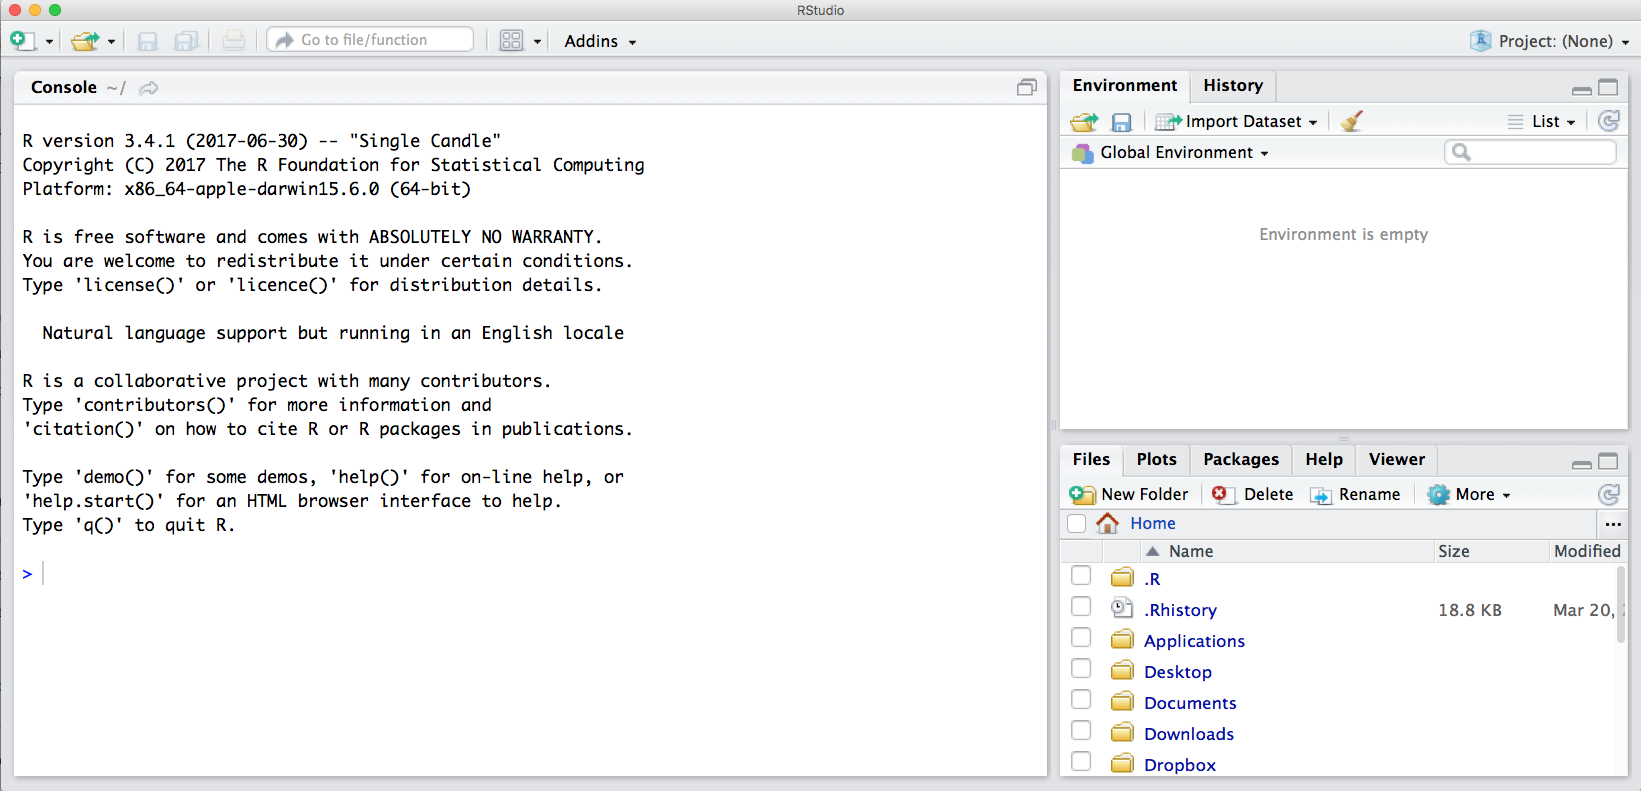
\includegraphics[width=0.8\linewidth]{img/RStudio_IDE}

Notice the default panes:

\begin{itemize}
\tightlist
\item
  Console (entire left)
\item
  Environment/History (tabbed in upper right)
\item
  Files/Plots/Packages/Help (tabbed in lower right)
\end{itemize}

FYI: you can change the default location of the panes, among many other things: \href{https://support.rstudio.com/hc/en-us/articles/200549016-Customizing-RStudio}{Customizing RStudio}.

An important first question: \textbf{where are we?}

If you've have opened RStudio for the first time, you'll be in your Home directory. This is noted by the \texttt{\textasciitilde{}/} at the top of the console. You can see too that the Files pane in the lower right shows what is in the Home directory where you are. You can navigate around within that Files pane and explore, but note that you won't change where you are: even as you click through you'll still be Home: \texttt{\textasciitilde{}/}.

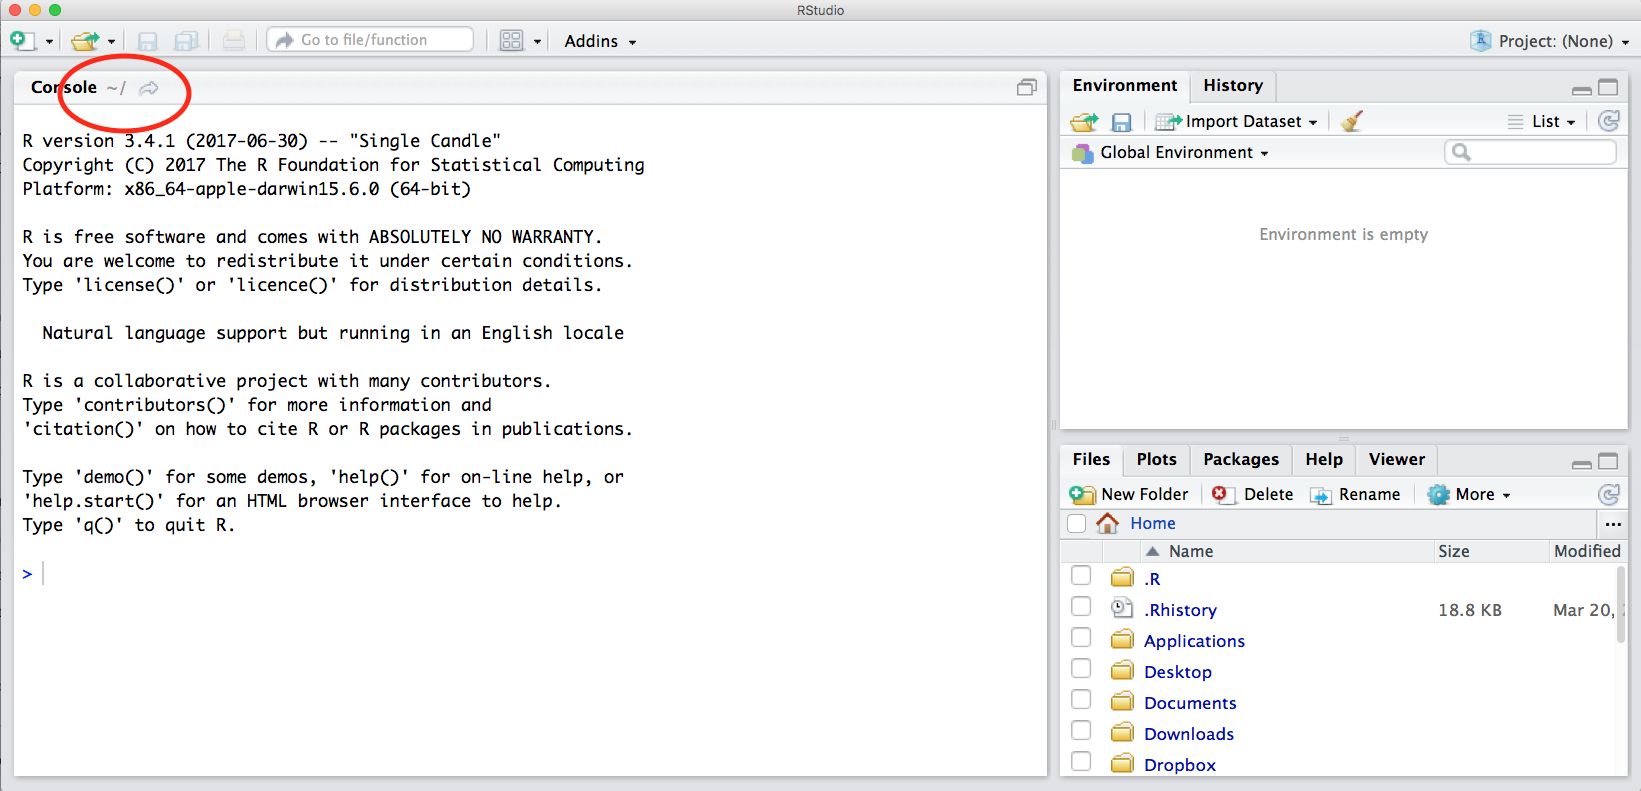
\includegraphics[width=0.8\linewidth]{img/RStudio_IDE_homedir}

\hypertarget{r-console}{%
\subsection{R Console}\label{r-console}}

Watch me work in the Console.

I can do math:

\begin{Shaded}
\begin{Highlighting}[]
\DecValTok{52}\OperatorTok{*}\DecValTok{40}
\DecValTok{365}\OperatorTok{/}\DecValTok{12}
\end{Highlighting}
\end{Shaded}

\emph{TODO: refine}

But like Excel, the power comes not from doing small operations by hand (like 8*22.3), it's by being able to operate on whole suites of numbers and datasets. In Excel, data are stored in the spreadsheet. In R, they are stored in dataframes, and named as variables.

R stores data in variables, and you give them names. This is a big difference with Excel, where you usually identify data by by its location on the grid, like \texttt{\$A1:D\$20}. (You can do this with Excel by naming ranges of cells, but most people don't do this.)

Data can be a variety of formats, like numeric and text.

Let's have a look at some data in R. R has several built-in data sets that we can look at and work with.

One of these datasets is called \texttt{mtcars}. If I write this in the Console, it will print the data in the console.

\begin{Shaded}
\begin{Highlighting}[]
\NormalTok{mtcars}
\end{Highlighting}
\end{Shaded}

I can also use RStudio's Viewer to see this in a more familiar-looking format:

\begin{Shaded}
\begin{Highlighting}[]
\KeywordTok{View}\NormalTok{(mtcars)}
\end{Highlighting}
\end{Shaded}

This opens the fourth pane of the RStudio IDE; when you work in R you will have all four panes open so this will become a very comforting setup for you.

\begin{quote}
The basic R data structure is a vector. You can think of a vector like a column in an Excel spreadsheet with the limitation that all the data in that vector must be of the same type. If it is a character vector, every element must be a character; if it is a logical vector, every element must be TRUE or FALSE; if it's numeric you can trust that every element is a number. There's no such constraint in Excel: you might have a column which has a bunch of numbers, but then some explanatory test intermingled with the numbers. This isn't allowed in R. - \url{https://blog.shotwell.ca/posts/r_for_excel_users/}
\end{quote}

In the Viewer I can do things like filter or sort. This does not do anything to the actual data, it just changes how you are viewing the data. So even as I explore it, I am not editing or manipulating the data.

Like Excel, some of the biggest power in R is that there are built-in functions that you can use in your analyses (and, as we'll see, R users can easily create and share functions, and it is this open source developer and contributor community that makes R so awesome).

So let's look into some of these functions. In Excel, there is a ``SUM'' function to calculate a total. Let's expect that there is the same in R. I will type this into the Console:

\begin{Shaded}
\begin{Highlighting}[]
\NormalTok{?sum}
\end{Highlighting}
\end{Shaded}

A few important things to note:

\begin{enumerate}
\def\labelenumi{\arabic{enumi}.}
\item
  R is case-sensitive. So ``sum'' is a completely different thing to ``Sum'' or ``SUM''. And this is true for the names of functions, data sets, variable names, and data itself (``blue'' vs ``Blue'').
\item
  RStudio has an autocomplete feature that can help you find the function you're looking for. In many cases it pops up as you type, but you can always type the tab key (above your caps lock key) to prompt the autocomplete. And, bonus: this feature can help you with the case-sensitivity mentioned above: If I start typing ``?SU'' and press tab, it will show me all options starting with those two letters, regardless of capitalization (although it will start with the capital S options).
\end{enumerate}

OK but what does typing \texttt{?sum} actually \emph{do}?

When I press enter/return, it will open up a help page in the bottom right pane. Help pages vary in detail I find some easier to digest than others. But they all have the same structure, which is helpful to know. The help page tells the name of the package in the top left, and broken down into sections:

\begin{itemize}
\tightlist
\item
  Description: An extended description of what the function does.
\item
  Usage: The arguments of the function and their default values.
\item
  Arguments: An explanation of the data each argument is expecting.
\item
  Details: Any important details to be aware of.
\item
  Value: The data the function returns.
\item
  See Also: Any related functions you might find useful.
\item
  Examples: Some examples for how to use the function.
\end{itemize}

When I look at a help page, I start with the description, which might be too in-the-weeds for the level of understanding I need at the offset. For the \texttt{sum} page, it is pretty straight-forward and lets me know that yup, this is the function I want.

I next look at the usage and arguments, which give me a more concrete view into what the function does. This syntax looks a bit cryptic but what it means is that you use it by writing sum, and then passing whatever you want to it in terms of data: that is what the ``\ldots{}'' means. And the ``na.rm=FALSE'' means that by default, it will not remove NAs (I read this as: ``remove NAs? FALSE!'')

Then, I usually scroll down to the bottom to the examples. This is where I can actually see how the function is used, and I can also paste those examples into the Console to see their output. Best way to learn what the function actually does is seeing it in action. Let's try:

\begin{Shaded}
\begin{Highlighting}[]
\KeywordTok{sum}\NormalTok{(}\DecValTok{1}\OperatorTok{:}\DecValTok{5}\NormalTok{)}
\end{Highlighting}
\end{Shaded}

So this is calculating the sum of the numbers from 1 and 5; that is what that \texttt{1:5} syntax means in this case. We can check it with the next example:

\begin{Shaded}
\begin{Highlighting}[]
\KeywordTok{sum}\NormalTok{(}\DecValTok{1}\NormalTok{, }\DecValTok{2}\NormalTok{, }\DecValTok{3}\NormalTok{, }\DecValTok{4}\NormalTok{, }\DecValTok{5}\NormalTok{)}
\end{Highlighting}
\end{Shaded}

Awesome. Let's try this on our \texttt{mtcars} data

\begin{Shaded}
\begin{Highlighting}[]
\KeywordTok{sum}\NormalTok{(mtcars)}
\end{Highlighting}
\end{Shaded}

Alright. What is this number? It is the sum of ALL of the data in the mtcars dataset. Maybe in some analysis this would be a useful operation, but I would worry about the way your data is set up and your analyses if this is ever something you'd want to do. More likely, you'd want to take the sum of a specific column. In R, you can do that with the \texttt{\$} operator.

Let's say we want to calculate the total number of gears that all these cars have:

\begin{Shaded}
\begin{Highlighting}[]
\KeywordTok{sum}\NormalTok{(mtcars}\OperatorTok{$}\NormalTok{gear)}
\end{Highlighting}
\end{Shaded}

\hypertarget{deep-thought}{%
\section{Deep thought}\label{deep-thought}}

How would you do this in Excel?
The calculations are usually the same shape as the data. In other words if you want to multiply 20 numbers stored in cells A1:An by 2, you will need 20 calculations: =A1 * 2, =A2 * 2, \ldots{}., =An * 2.

OK so now that we've got a little bit of a feel for R and RStudio, let's do something much more interesting and really start feeling its power.

---\textgreater{}

\hypertarget{deep-thought-error-messages-are-your-friends}{%
\subsection{Deep thought: Error messages are your friends}\label{deep-thought-error-messages-are-your-friends}}

As \href{https://stat545.com/r-basics.html}{Jenny Bryan says}:

\begin{quote}
Implicit contract with the computer / scripting language: Computer will do tedious computation for you. In return, you will be completely precise in your instructions. Typos matter. Case matters. Pay attention to how you type.
\end{quote}

Remember that this is a language, not unsimilar to English! There are times you aren't understood -- it's going to happen. There are different ways this can happen. Sometimes you'll get an error. This is like someone saying `What?' or `Pardon'? Error messages can also be more useful, like when they say `I didn't understand what you said, I was expecting you to say blah'. That is a great type of error message. Error messages are your friend. Google them (copy-and-paste!) to figure out what they mean.

And also know that there are errors that can creep in more subtly, when you are giving information that is understood, but not in the way you meant. Like if I am telling a story about suspenders that my British friend hears but silently interprets in a very different way (true story). This can leave me thinking I've gotten something across that the listener (or R) might silently interpreted very differently. And as I continue telling my story you get more and more confused\ldots{} Clear communication is critical when you code: write clean, well documented code and check your work as you go to minimize these circumstances!

\hypertarget{dont-save-the-workspace}{%
\section{Don't save the workspace}\label{dont-save-the-workspace}}

\hypertarget{deep-thought-keep-the-raw-data-raw.}{%
\section{Deep thought: keep the raw data raw.}\label{deep-thought-keep-the-raw-data-raw.}}

Discussing using Excel for variables.

Horror Stories! Economist etc. --

Mine: genetics example doesn't hit home as much as Durham bike accidents where age groups are converted to dates just by opening the bloody csv in excel

\hypertarget{activity-1}{%
\section{Activity 1}\label{activity-1}}

\hypertarget{activity-2}{%
\section{Activity 2}\label{activity-2}}

\hypertarget{efficiency-tips}{%
\section{Efficiency Tips}\label{efficiency-tips}}

\hypertarget{troubleshooting}{%
\section{Troubleshooting}\label{troubleshooting}}

Here are some additional things we didn't have time to discuss:

\hypertarget{i-entered-a-command-and-nothings-happening}{%
\subsection{I entered a command and nothing's happening}\label{i-entered-a-command-and-nothings-happening}}

It may be because you didn't complete a command: is there a little \texttt{+} in your console? R is saying that it is waiting for you to finish. In the example below, I need to close that parenthesis.

\begin{Shaded}
\begin{Highlighting}[]
\OperatorTok{>}\StringTok{ }\NormalTok{x <-}\StringTok{ }\KeywordTok{seq}\NormalTok{(}\DecValTok{1}\NormalTok{, }\DecValTok{10}
\OperatorTok{+}\StringTok{ }
\end{Highlighting}
\end{Shaded}

\hypertarget{rstudio}{%
\chapter{R \& RStudio, RMarkdown}\label{rstudio}}

TODO: Intro: we're going to start off with RMarkdown.

TODO: break into ``R chunks'' and ``Markdown sections''

TODO: harmonize with OHI's training

Introduce projects and setup data/ folder

TODO (write out):
Intro, knitting
How in-line figures are awesome (no copy-pasting from excel to word)
Reproducibility is important (this might be new to some people). Reproducible research/self-contained Rmd files: read in data at the top. Read\_csv.

\hypertarget{summary-1}{%
\section{Summary}\label{summary-1}}

We'll learn RMarkdown, which helps you tell a story with your data analysis because you can write text alongside the code. We are actually learning two languages at once: R and Markdown.

\hypertarget{objectives-more-detailed-bulletpoints-1}{%
\section{Objectives (more detailed, bulletpoints?)}\label{objectives-more-detailed-bulletpoints-1}}

\hypertarget{resources-1}{%
\section{Resources}\label{resources-1}}

\hypertarget{intro-to-rmarkdown}{%
\section{Intro to RMarkdown}\label{intro-to-rmarkdown}}

An RMarkdown file will allow us to weave markdown text with chunks of R code to be evaluated and output content like tables and plots. This is super cool, and really best to experience before we talk about it. So let's do this together.

\hypertarget{create-an-rmarkdown-file}{%
\subsection{Create an RMarkdown file}\label{create-an-rmarkdown-file}}

File -\textgreater{} New File -\textgreater{} RMarkdown\ldots{} -\textgreater{} Document of output format HTML, OK.

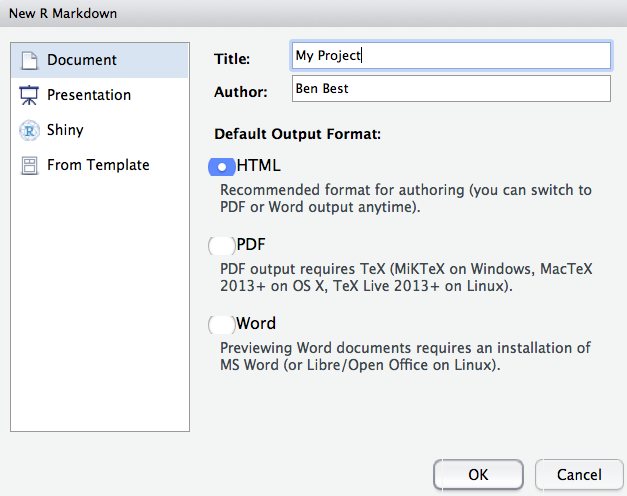
\includegraphics[width=0.8\linewidth]{img/rstudio_new-rmd-doc-html}

You can give it a Title like ``Testing'' (a name that's totally ok to use as you're trying something out). Then click OK.

OK, first off: by opening a file, we are seeing the 4th pane of the RStudio console, which is essentially a text editor. This lets us organize our files within RStudio instead of having a bunch of different windows open.

Let's have a look at this file --- it's not blank; there is some initial text is already provided for you. Notice a few things about it:

\begin{itemize}
\tightlist
\item
  Title and Author are auto-filled, and the today's date has been added
\item
  There are white and grey sections. These are the 2 main languages that make up an RMarkdown file.

  \begin{itemize}
  \tightlist
  \item
    \textbf{Grey sections are R code}
  \item
    \textbf{White sections are Markdown text}
  \end{itemize}
\end{itemize}

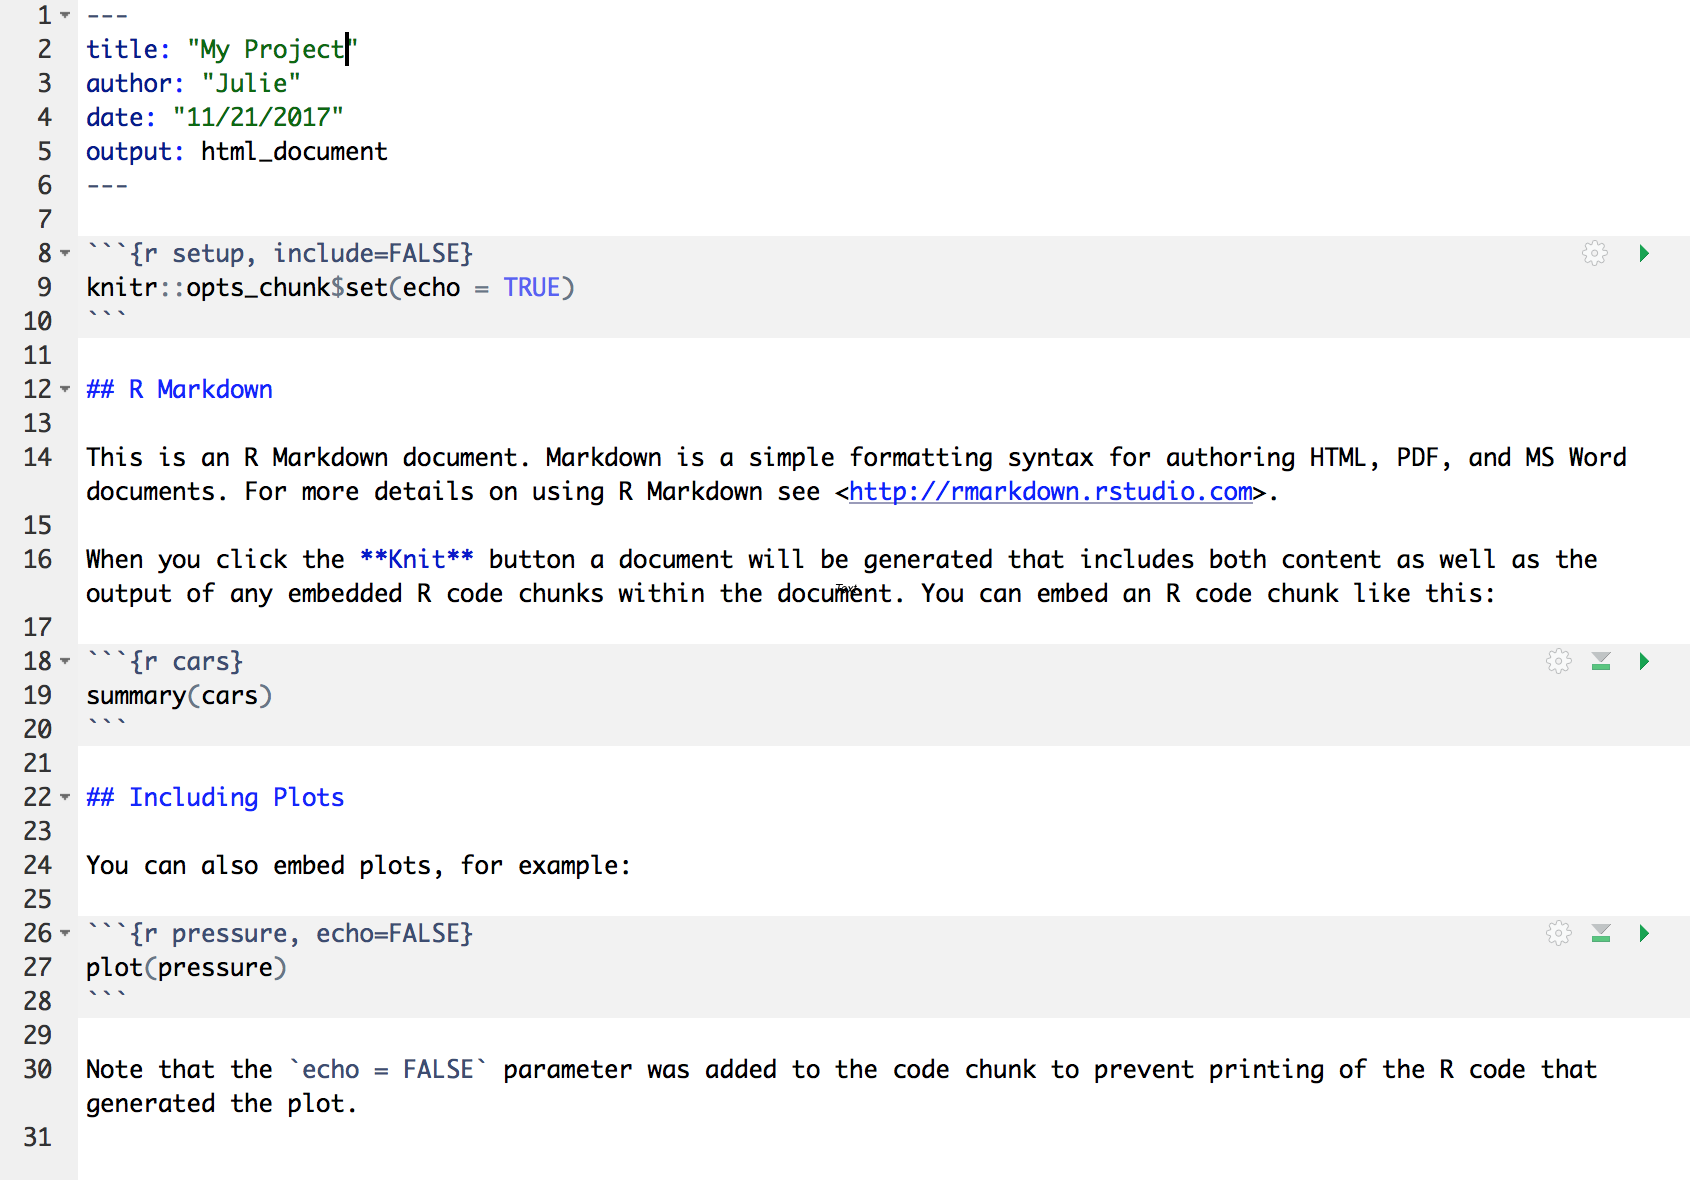
\includegraphics[width=0.8\linewidth]{img/rmarkdown}

\hypertarget{knit-your-rmarkdown-file}{%
\subsection{Knit your RMarkdown file}\label{knit-your-rmarkdown-file}}

Let's go ahead and ``Knit'' by clicking the blue yarn at the top of the RMarkdown file. It's going to ask us to save first, I'll name mine ``testing.Rmd''.

How cool is this, we've just made an html file, a webpage that we are viewing locally on our own computers. Knitting this RMarkdown document has rendered --- we also say formatted --- both the Markdown text (white) and the R code (grey), and the it also executed --- we also say ran --- the R code.

Let's have a look at them side-by-side:

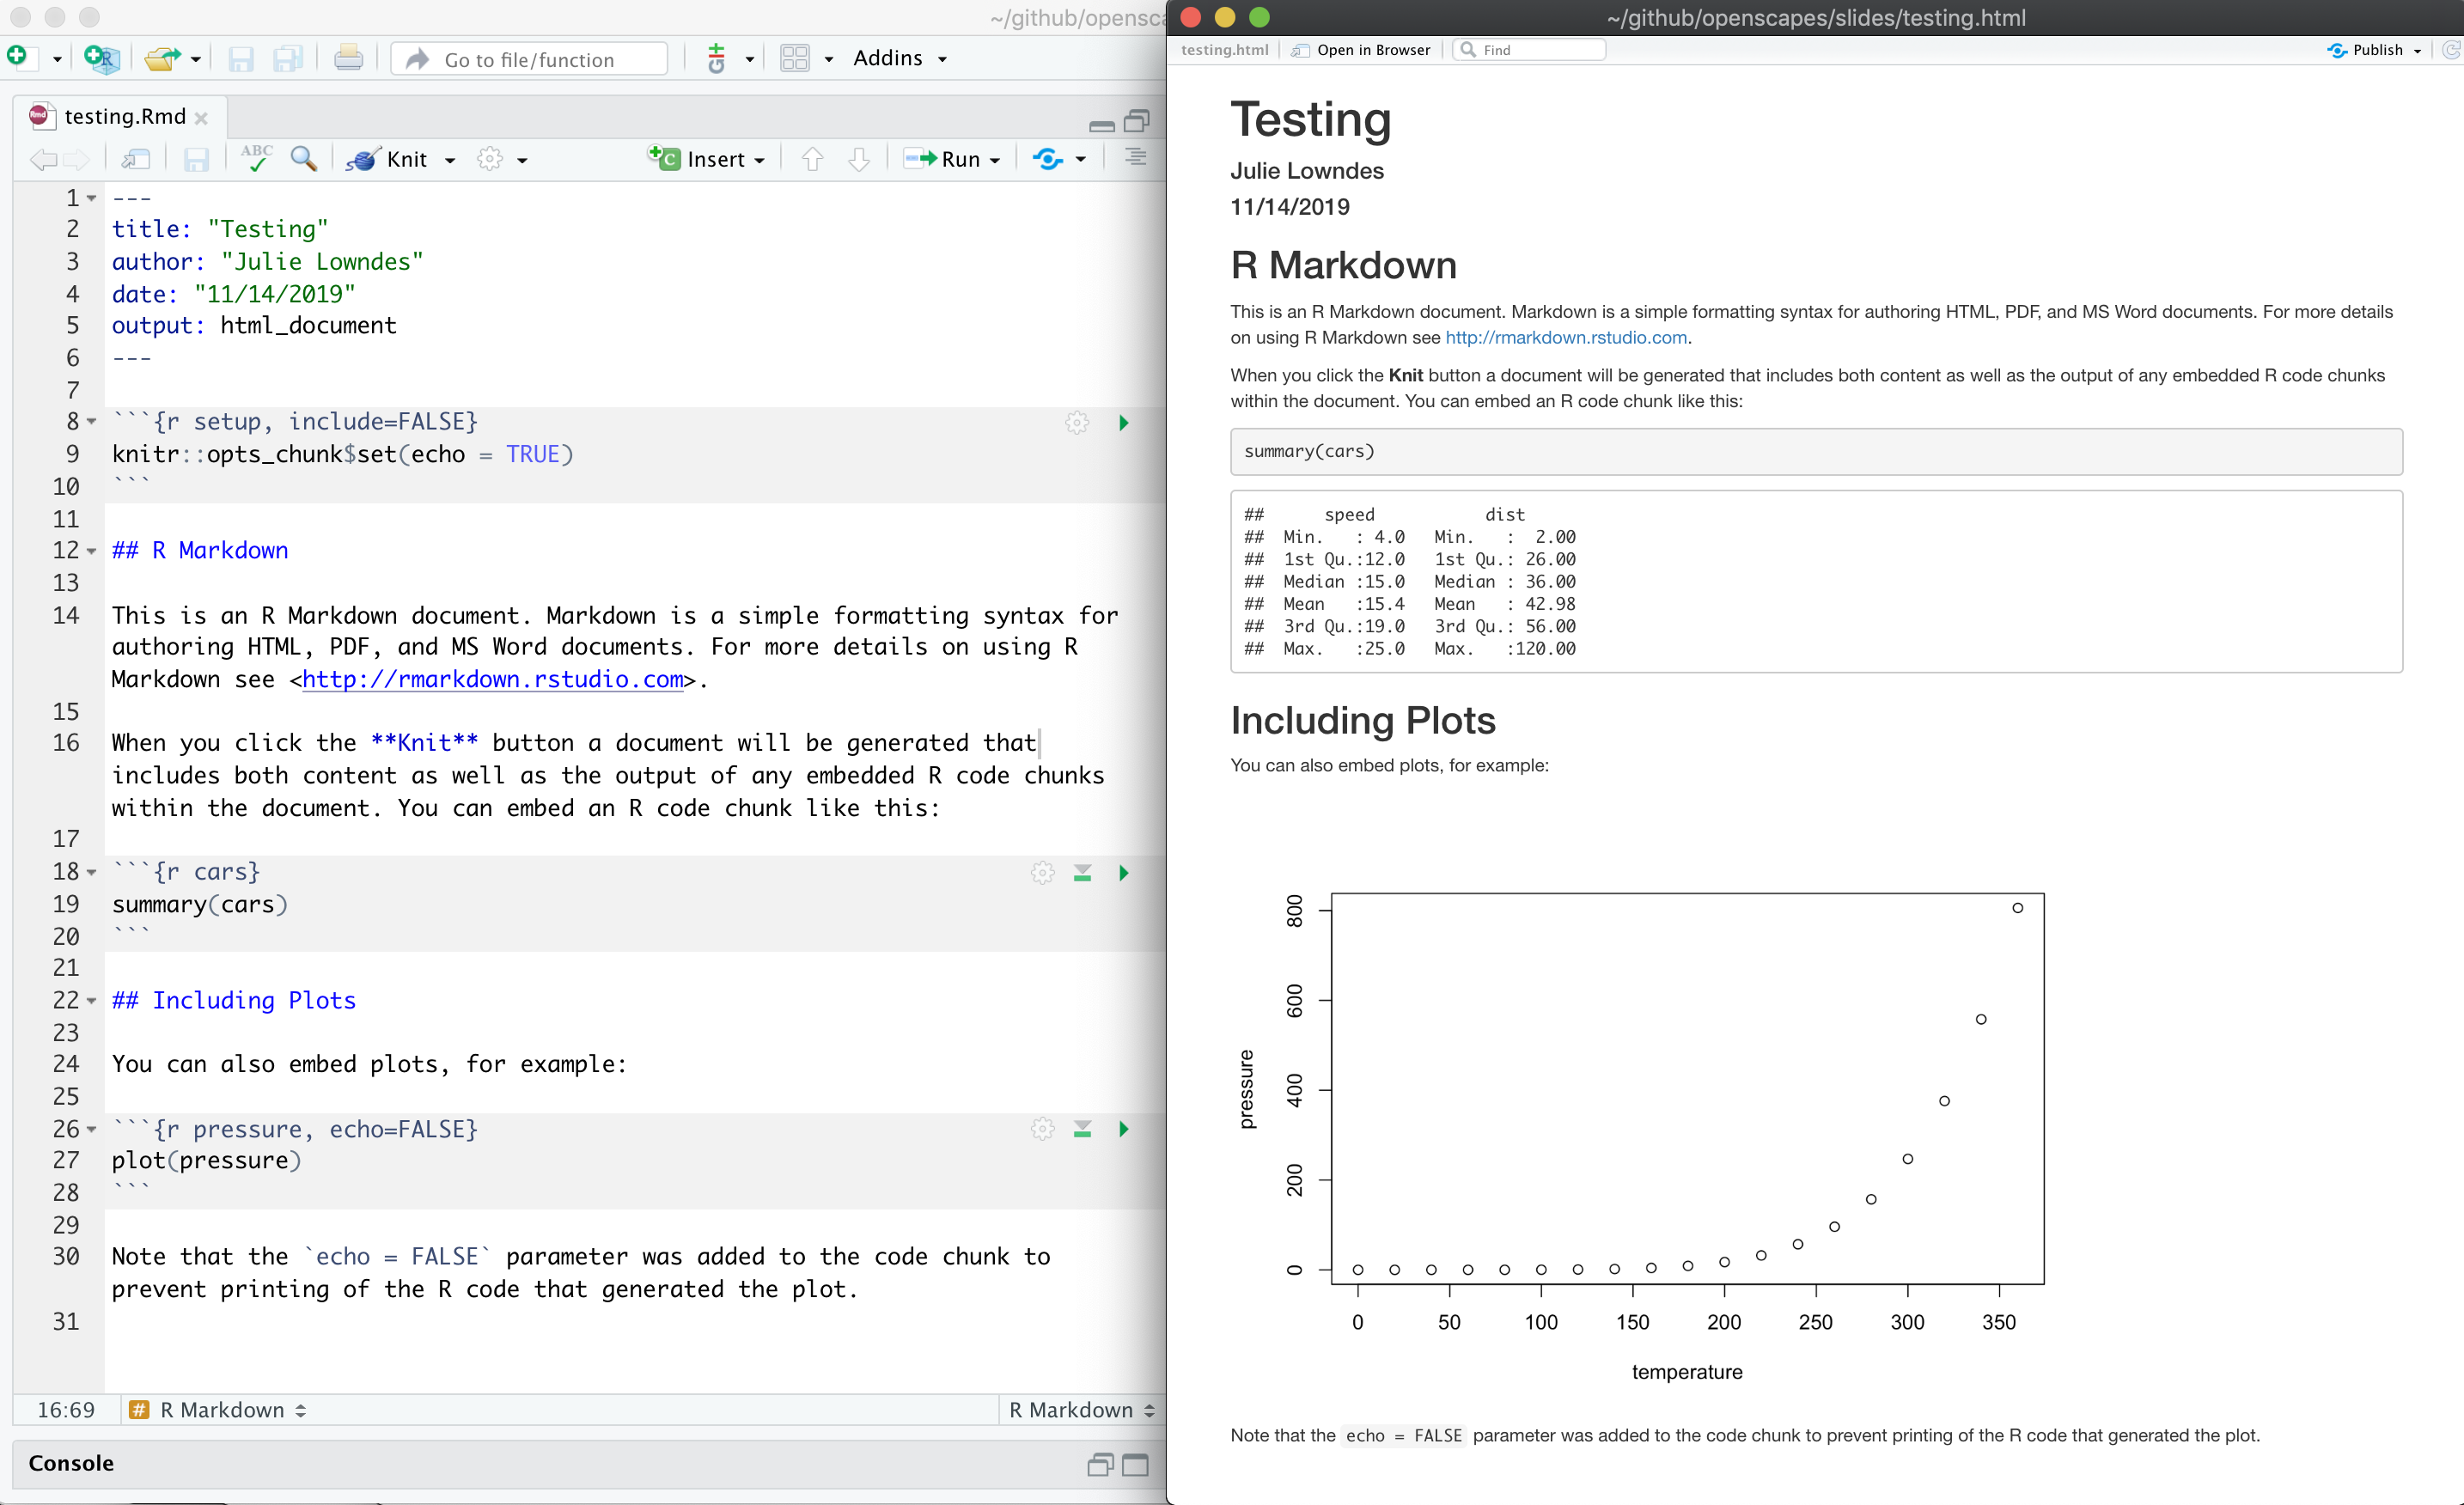
\includegraphics[width=0.8\linewidth]{img/rmarkdown_side_by_side}

Let's take a deeper look at these two files. So much of learning to code is looking for patterns.

\hypertarget{activity-5-mins}{%
\subsection{Activity (5 mins)}\label{activity-5-mins}}

Look at these two files while talking with your neighbor: What do you notice between the two files? Start off with these observations:

\begin{itemize}
\tightlist
\item
  Markdown text (white sections): The two hashtags \texttt{\#\#} cause the following text to be displayed as a header: the text is larger and in bold
\item
  R code (grey sections): The \texttt{summary()} function outputs summary statistics and the \texttt{plot()} function creates a plot!
\end{itemize}

And now let's talk about this.

\hypertarget{r-code-chunks}{%
\subsection{R code chunks}\label{r-code-chunks}}

Notice how the grey \textbf{R code chunks} are surrounded by 3 backticks and \texttt{\{r\ LABEL\}}. These are evaluated and return the output text in the case of \texttt{summary(cars)} and the output plot in the case of \texttt{plot(pressure)}.

Notice how the code \texttt{plot(pressure)} is not shown in the HTML output because of the R code chunk option \texttt{echo=FALSE}.
COME BACK!!!

We don't know that much R yet, but you can see that we are taking a summary of some data called `cars', and then plotting. We will focus on R for the rest of the workshop, but for the rest of this morning let's focus on the second language.

The second language is Markdown. This is a formatting language for plain text, and there are only about 15 rules to know.

Notice the syntax for:

\begin{itemize}
\tightlist
\item
  \textbf{headers} get rendered at multiple levels: \texttt{\#}, \texttt{\#\#}
\item
  \textbf{bold}: \texttt{**word**}
\end{itemize}

There are some good \href{https://github.com/adam-p/markdown-here/wiki/Markdown-Here-Cheatsheet}{cheatsheets} to get you started, and here is one built into RStudio: Go to Help \textgreater{} Markdown Quick Reference

\textbf{Important}: note that the hashtag \texttt{\#} is used differently in Markdown and in R:

\begin{itemize}
\tightlist
\item
  in R, a hashtag indicates a comment that will not be evaluated. You can use as many as you want: \texttt{\#} is equivalent to \texttt{\#\#\#\#\#\#}. It's a matter of style. I use two \texttt{\#\#} to indicate a comment so that it's clearer what is a comment versus what I don't want to run at the moment.
\item
  in Markdown, a hashtag indicates a level of a header. And the number you use matters: \texttt{\#} is a ``level one header'', meaning the biggest font and the top of the hierarchy. \texttt{\#\#\#} is a level three header, and will show up nested below the \texttt{\#} and \texttt{\#\#} headers.
\end{itemize}

If this seems confusing, take comfort in the fact that you are already used to using \texttt{\#}s differently in real life: it can mean ``number'' or ``pound'' or hashtags on social media.

Learn more: \url{http://rmarkdown.rstudio.com/}

\hypertarget{activity}{%
\subsection{Activity}\label{activity}}

\begin{enumerate}
\def\labelenumi{\arabic{enumi}.}
\tightlist
\item
  In Markdown write some italic text, make a numbered list, and add a few subheaders.
  Use the Markdown Quick Reference (in the menu bar: Help \textgreater{} Markdown Quick Reference).
\item
  Reknit your html file.
\end{enumerate}

\hypertarget{r-chunks}{%
\subsection{R chunks}\label{r-chunks}}

OK. Now let's practice with some of those commands that we were working on this morning.

Create a new chunk in your RMarkdown first in one of these ways:

\begin{itemize}
\tightlist
\item
  click ``Insert \textgreater{} R'' at the top of the editor pane
\item
  type by hand
  ```\{r\}
  ```
\item
  if you haven't deleted a chunk that came with the new file, edit that one
\end{itemize}

Now, let's write some R code.

\begin{verbatim}
x <- seq(1:15)
\end{verbatim}

Now, hitting return does not execute this command; remember, it's a text file in the text editor, it's not associated with the R engine. To execute it, we need to get what we typed in the the R chunk (the grey R code) down into the console. How do we do it? There are several ways (let's do each of them):

\begin{enumerate}
\def\labelenumi{\arabic{enumi}.}
\tightlist
\item
  copy-paste this line into the console.
\item
  select the line (or simply put the cursor there), and click `Run'. This is available from

  \begin{enumerate}
  \def\labelenumii{\alph{enumii}.}
  \tightlist
  \item
    the bar above the file (green arrow)
  \item
    the menu bar: Code \textgreater{} Run Selected Line(s)
  \item
    keyboard shortcut: command-return
  \end{enumerate}
\item
  click the green arrow at the right of the code chunk
\end{enumerate}

Cool tip: doesn't have to be only R, other languages supported.

\hypertarget{activity-3}{%
\subsection{Activity}\label{activity-3}}

\begin{quote}
Add a few more commands to your file from this morning. Execute them by trying the three ways above. Then, knit your R Markdown file, which will also save the Rmd by default.
\end{quote}

\hypertarget{activity-4}{%
\section{Activity}\label{activity-4}}

\begin{enumerate}
\def\labelenumi{\arabic{enumi}.}
\tightlist
\item
  knit!
\end{enumerate}

Delete everything! Just by being an .Rmd file, this will knit

\hypertarget{deep-thoughts}{%
\section{Deep thoughts}\label{deep-thoughts}}

Command-Z is the best

\hypertarget{fun-facts-quirky-things---making-a-note-of-these-wherever-possible-for-interest-little-did-you-know-sections}{%
\section{Fun facts (quirky things) - making a note of these wherever possible for interest (little ``Did you know?'' sections)}\label{fun-facts-quirky-things---making-a-note-of-these-wherever-possible-for-interest-little-did-you-know-sections}}

\hypertarget{interludes-deep-thoughtsopenscapes}{%
\section{Interludes (deep thoughts/openscapes)}\label{interludes-deep-thoughtsopenscapes}}

\hypertarget{interludes-deep-thoughtsopenscapes-1}{%
\section{Interludes (deep thoughts/openscapes)}\label{interludes-deep-thoughtsopenscapes-1}}

Comments! Organization (spacing, subsections, vertical structure, indentation, etc.)! Well-named variables! Also, well-named operations so analyses (select(data, columnname)) instead of data{[}1:6,5{]} and excel equivalent. (Ex with strings)
Not so brittle/sensitive to minor changes.

\hypertarget{rmarkdown-video-1-minute}{%
\subsection{RMarkdown video (1-minute)}\label{rmarkdown-video-1-minute}}

Let's watch this to demonstrate all the amazing things you can now do:

\href{https://vimeo.com/178485416}{What is RMarkdown?}

\hypertarget{efficiency-tips-1}{%
\section{Efficiency Tips}\label{efficiency-tips-1}}

\hypertarget{github}{%
\chapter{GitHub}\label{github}}

Setup GitHub
GitHub
Scrap plans for publishing and issues: setup version control and practice like OHI data-science-training.
Practice committing the README and .gitignore
Copy our rproj into this repo and push

Add at the end: create an Rmd for our next lesson after lunch? Yes, and add a header with their inform

Create the github repo: `r-and-excel'

\hypertarget{reading}{%
\subsection{Reading}\label{reading}}

\hypertarget{fun-facts-quirky-things---making-a-note-of-these-wherever-possible-for-interest-little-did-you-know-sections-1}{%
\section{Fun facts (quirky things) - making a note of these wherever possible for interest (little ``Did you know?'' sections)}\label{fun-facts-quirky-things---making-a-note-of-these-wherever-possible-for-interest-little-did-you-know-sections-1}}

\hypertarget{interludes-deep-thoughtsopenscapes-2}{%
\section{Interludes (deep thoughts/openscapes)}\label{interludes-deep-thoughtsopenscapes-2}}

\hypertarget{our-turn-your-turn-1}{%
\section{Our Turn Your Turn 1}\label{our-turn-your-turn-1}}

\hypertarget{our-turn-your-turn-2}{%
\section{Our Turn Your Turn 2}\label{our-turn-your-turn-2}}

\hypertarget{efficiency-tips-2}{%
\section{Efficiency Tips}\label{efficiency-tips-2}}

\hypertarget{readxl}{%
\chapter{\texorpdfstring{\texttt{readxl}}{readxl}}\label{readxl}}

\hypertarget{summary-2}{%
\section{Summary}\label{summary-2}}

\textbf{Check this, may need to be a block quote}: The \textbf{readxl} package makes it easy to import tabular data from Excel spreadsheets (.xls or .xlsx files) and includes several options for cleaning data during import. \textbf{readxl} has no external dependencies and functions on any operating system, making it an OS- and user-friendly package that simplifies getting your data from Excel into R.

\hypertarget{objectives}{%
\section{Objectives}\label{objectives}}

\begin{itemize}
\tightlist
\item
  Use \texttt{readr::read\_csv()} to read in a comma separated value (CSV) file
\item
  Use \texttt{readxl::read\_excel()} to read in an Excel worksheet from a workbook
\item
  Replace a specific string/value in a spreadsheet with with \texttt{NA}
\item
  Skip \emph{n} rows when importing an Excel worksheet
\item
  Use \texttt{readxl::read\_excel()} to read in parts of a worksheet (by cell range)
\item
  Specify column names when importing Excel data
\item
  Read and combine data from multiple Excel worksheets into a single df using \texttt{purrr::map\_df()}
\item
  Write data using \texttt{readr::write\_csv()} or \texttt{writexl::write\_xlsx()}
\item
  Workflows with \texttt{readxl}: considerations, limitations, reproducibility
\end{itemize}

\hypertarget{resources-2}{%
\section{Resources}\label{resources-2}}

\begin{itemize}
\tightlist
\item
  \url{https://readxl.tidyverse.org/}
\item
  \href{https://readxl.tidyverse.org/articles/articles/readxl-workflows.html}{readxl Workflows article (from tidyverse.org)}
\end{itemize}

\hypertarget{lesson}{%
\section{Lesson}\label{lesson}}

\hypertarget{lesson-prep-get-data-files-into-your-working-directory}{%
\subsection{Lesson prep: get data files into your working directory}\label{lesson-prep-get-data-files-into-your-working-directory}}

In Session 1, we introduced how and why R Projects are great for reproducibility, because our self-contained working directory will be the \textbf{first} place R looks for files.

You downloaded TODO: XX files for this workshop:

\begin{itemize}
\tightlist
\item
  fish\_counts\_curated.csv
\item
  invert\_counts\_curated.xlsx
\item
  kelp\_counts\_curated.xlsx
\item
  substrate\_cover\_curated.xlsx
\item
  lobster\_counts.csv TODO: add this?
\item
  national\_parks.xlsx TODO: add this?
\end{itemize}

Copy and paste those files into the `r-and-excel' folder on your computer. Notice that now these files are in your working directory when you go back to that Project in RStudio (check the `Files' tab). That means they're going to be in the first place R will look when you ask it to find a file to read in.

\hypertarget{in-the-.rmd-you-just-created-attach-the-tidyverse-readxl-and-writexl-packages}{%
\subsection{\texorpdfstring{In the .Rmd you just created, attach the \texttt{tidyverse}, \texttt{readxl} and \texttt{writexl} packages}{In the .Rmd you just created, attach the tidyverse, readxl and writexl packages}}\label{in-the-.rmd-you-just-created-attach-the-tidyverse-readxl-and-writexl-packages}}

In this lesson, we'll read in a CSV file with the \texttt{readr::read\_csv()} function, so we need to have the \texttt{readr} package attached. Since it's part of the \texttt{tidyverse}, we'll go ahead and attach the \texttt{tidyverse} package below our script header using \texttt{library(package\_name)}. It's a good idea to attach packages within the set-up chunk in R Markdown, so we'll also attach the \texttt{readxl} and \texttt{writexl}packages there.

Here's our first code chunk:

\begin{verbatim}
{r setup, eval = FALSE}
knitr::opts_chunk$set(echo = TRUE)

# Attach the tidyverse, readxl and writexl packages:
library(tidyverse)
library(readxl)
library(writexl)
\end{verbatim}

Now, all of the packages and functions within the \texttt{tidyverse} and \texttt{readxl}, including \texttt{readr::read\_csv()} and \texttt{readxl::read\_excel()}, are available for use.

\hypertarget{use-readrread_csv-to-read-in-data-from-a-csv-file}{%
\subsection{\texorpdfstring{Use \texttt{readr::read\_csv()} to read in data from a CSV file}{Use readr::read\_csv() to read in data from a CSV file}}\label{use-readrread_csv-to-read-in-data-from-a-csv-file}}

There are many types of files containing data that you might want to work with in R. A common one is a comma separated value (CSV) file, which contains values with each column entry separated by a comma delimiter. CSVs can be opened, viewed, and worked with in Excel just like an .xls or .xlsx file - but let's learn how to get data directly from a CSV into R where we can work with it more reproducibly.

The CSV we'll read in here is called ``fish\_counts\_curated.csv'', and contains observations for ``the abundance and size of fish species as part of SBCLTER's kelp forest monitoring program to track long-term patterns in species abundance and diversity'' from the \href{http://sbc.lternet.edu/}{Santa Barbara Channel Long Term Ecological Research} program.

\textbf{Source:} Reed D. 2018. SBC LTER: Reef: Kelp Forest Community Dynamics: Fish abundance. Environmental Data Initiative. \url{https://doi.org/10.6073/pasta/dbd1d5f0b225d903371ce89b09ee7379}. Dataset accessed 9/26/2019.

Read in the ``fish\_counts\_curated.csv'' file \texttt{read\_csv("file\_name.csv")}, and store it in R as an object called \emph{fish\_counts}:

\begin{Shaded}
\begin{Highlighting}[]
\NormalTok{fish_counts <-}\StringTok{ }\KeywordTok{read_csv}\NormalTok{(}\StringTok{"fish_counts_curated.csv"}\NormalTok{)}
\end{Highlighting}
\end{Shaded}

Notice that the name of the stored object (here, \emph{fish\_counts}) will show up in our Environment tab in RStudio.

Click on the object in the Environment, and R will automatically run the \texttt{View()} function for you to pull up your data in a separate viewing tab. Now we can look at it in the spreadsheet format we're used to.

Here are a few other functions for quickly exploring imported data:

\begin{itemize}
\tightlist
\item
  \texttt{summary()}: summary of class, dimensions, \texttt{NA} values, etc.
\item
  \texttt{names()}: variable names (column headers)
\item
  \texttt{ls()}: list all objects in environment
\item
  \texttt{head()}: Show the first x rows (default is 6 lines)
\item
  \texttt{tail()}: Show the last x rows (default is 6 lines)
\end{itemize}

Now that we have our fish counts data ready to work with in R, let's get the substrate cover and kelp data (both .xlsx files). In the following sections, we'll learn that we can use \texttt{readxl::read\_excel()} to read in Excel files directly.

\hypertarget{use-readxlread_excel-to-read-in-a-single-excel-worksheet}{%
\subsection{\texorpdfstring{Use \texttt{readxl::read\_excel()} to read in a single Excel worksheet}{Use readxl::read\_excel() to read in a single Excel worksheet}}\label{use-readxlread_excel-to-read-in-a-single-excel-worksheet}}

First, take a look at \emph{substrate\_cover\_curated.xlsx} in Excel, which contains a single worksheet with substrate type and percent cover observations at different sampling locations in the Santa Barbara Channel.

A few things to notice:

\begin{itemize}
\tightlist
\item
  The file contains a single worksheet
\item
  There are multiple rows containing text information up top
\item
  Where observations were not recorded, there exists `-9999'
\end{itemize}

Let's go ahead and read in the data. If the file is in our working directory, we can read in a single worksheet .xlsx file using \texttt{readxl::read\_excel("file\_name.xlsx")}. \emph{Note: readxl::read\_excel() works for both .xlsx and .xls types}.

Like this:

\begin{Shaded}
\begin{Highlighting}[]
\NormalTok{substrate_cover <-}\StringTok{ }\KeywordTok{read_excel}\NormalTok{(}\StringTok{"substrate_cover_curated.xlsx"}\NormalTok{)}
\end{Highlighting}
\end{Shaded}

\textbf{Tada? Not quite.}

Click on the object name (\emph{substrate\_cover}) in the Environment to view the data in a new tab. A few things aren't ideal:

\begin{Shaded}
\begin{Highlighting}[]
\NormalTok{substrate_cover}
\end{Highlighting}
\end{Shaded}

\begin{verbatim}
## # A tibble: 23,942 x 9
##    `Substrate cover data~ ...2  ...3   ...4  ...5   ...6  ...7  ...8  ...9 
##    <chr>                  <chr> <chr>  <chr> <chr>  <chr> <chr> <chr> <chr>
##  1 Source: https://porta~ <NA>  <NA>   <NA>  <NA>   <NA>  <NA>  <NA>  <NA> 
##  2 Accessed: 9/28/2019    <NA>  <NA>   <NA>  <NA>   <NA>  <NA>  <NA>  <NA> 
##  3 <NA>                   <NA>  <NA>   <NA>  <NA>   <NA>  <NA>  <NA>  <NA> 
##  4 year                   month date   site  trans~ quad  side  subs~ perc~
##  5 -9999                  -9999 -9999  carp  1      20    i     b     -9999
##  6 2000                   9     -9999  carp  1      20    o     b     -9999
##  7 2000                   9     9/8/00 carp  1      20    i     b     100  
##  8 2000                   9     9/8/00 carp  1      20    o     b     100  
##  9 2000                   9     9/8/00 carp  1      40    i     b     100  
## 10 2000                   9     9/8/00 carp  1      40    o     b     100  
## # ... with 23,932 more rows
\end{verbatim}

\begin{itemize}
\tightlist
\item
  The top row of text has automatically become the (messy) column headers
\item
  There are multiple descriptive rows before we actually get to the data
\item
  There are -9999s that we want R to understand \texttt{NA} instead
\end{itemize}

We can deal with those issues by adding arguments within \texttt{read\_excel()}. Include argument \texttt{skip\ =\ n} to skip the first `n' rows when importing data, and \texttt{na\ =\ "this"} to replace ``this'' with \texttt{NA} when importing:

\begin{Shaded}
\begin{Highlighting}[]
\NormalTok{substrate_cover <-}\StringTok{ }\KeywordTok{read_excel}\NormalTok{(}\StringTok{"curation/substrate_cover_curated.xlsx, skip = 4, na = "}\OperatorTok{-}\DecValTok{9999}\StringTok{")}
\end{Highlighting}
\end{Shaded}

\begin{Shaded}
\begin{Highlighting}[]
\NormalTok{substrate_cover}
\end{Highlighting}
\end{Shaded}

\begin{verbatim}
## # A tibble: 23,938 x 9
##    year  month date  site  transect quad  side  substrate_type
##    <chr> <chr> <chr> <chr> <chr>    <chr> <chr> <chr>         
##  1 <NA>  <NA>  <NA>  carp  1        20    i     b             
##  2 2000  9     <NA>  carp  1        20    o     b             
##  3 2000  9     9/8/~ carp  1        20    i     b             
##  4 2000  9     9/8/~ carp  1        20    o     b             
##  5 2000  9     9/8/~ carp  1        40    i     b             
##  6 2000  9     9/8/~ carp  1        40    o     b             
##  7 2000  9     9/8/~ carp  2        20    i     b             
##  8 2000  9     9/8/~ carp  2        20    o     b             
##  9 2000  9     9/8/~ carp  2        40    i     b             
## 10 2000  9     9/8/~ carp  2        40    o     b             
## # ... with 23,928 more rows, and 1 more variable: percent_cover <chr>
\end{verbatim}

Check out \emph{substrate\_cover}, and see that the first row \emph{after} the 4 skipped are the column names, and all -9999s have been updated to \texttt{NA}. Hooray!

\hypertarget{use-readxlread_excel-to-read-in-only-part-of-an-excel-worksheet}{%
\subsection{\texorpdfstring{Use \texttt{readxl::read\_excel()} to read in only \emph{part} of an Excel worksheet}{Use readxl::read\_excel() to read in only part of an Excel worksheet}}\label{use-readxlread_excel-to-read-in-only-part-of-an-excel-worksheet}}

We always advocate for leaving the raw data raw, and writing a complete script containing all steps of data wrangling \& transformation. But in \emph{some} situations (be careful), you may want to specify a range of cells to read in from an Excel worksheet.

You can specify a range of cells to read in using the \texttt{range\ =} argument in \texttt{read\_excel()}. For example, if I want to read in the rectangle from D12:I15 in \emph{substrate\_cover\_curated.xlsx} - only observations for Carpenteria Beach (Transect 2) in September 2000 - I can use:

\begin{Shaded}
\begin{Highlighting}[]
\NormalTok{carp_cover_}\DecValTok{2000}\NormalTok{ <-}\StringTok{ }\NormalTok{readxl}\OperatorTok{::}\KeywordTok{read_excel}\NormalTok{(}\StringTok{"substrate_cover_curated.xlsx"}\NormalTok{, }\DataTypeTok{range =} \StringTok{"D12:I15"}\NormalTok{)}
\end{Highlighting}
\end{Shaded}

But yuck. Look at \emph{carp\_cover\_2000} and you'll notice that the first row \emph{of that range} is automatically made the column headers. To keep all rows within a range and \textbf{add your own column names}, add a \texttt{col\_names\ =} argument:

\begin{Shaded}
\begin{Highlighting}[]
\NormalTok{carp_cover_}\DecValTok{2000}\NormalTok{ <-}\StringTok{ }\NormalTok{readxl}\OperatorTok{::}\KeywordTok{read_excel}\NormalTok{(}\StringTok{"substrate_cover_curated.xlsx"}\NormalTok{, }\DataTypeTok{range =} \StringTok{"D12:I15"}\NormalTok{, }\DataTypeTok{col_names =} \KeywordTok{c}\NormalTok{(}\StringTok{"site_name"}\NormalTok{, }\StringTok{"transect"}\NormalTok{, }\StringTok{"quad"}\NormalTok{, }\StringTok{"plot_side"}\NormalTok{, }\StringTok{"type"}\NormalTok{, }\StringTok{"coverage"}\NormalTok{))}
\end{Highlighting}
\end{Shaded}

\begin{Shaded}
\begin{Highlighting}[]
\NormalTok{carp_cover_}\DecValTok{2000}
\end{Highlighting}
\end{Shaded}

\begin{verbatim}
## # A tibble: 4 x 6
##   site_name transect quad  plot_side type  coverage
##   <chr>     <chr>    <chr> <chr>     <chr> <chr>   
## 1 carp      2        20    i         b     90      
## 2 carp      2        20    o         b     80      
## 3 carp      2        40    i         b     80      
## 4 carp      2        40    o         b     85
\end{verbatim}

So far we've read in a single CSV file using \texttt{readr::read\_csv()}, and an Excel file containing a single worksheet with \texttt{readxl::read\_excel()}. Now let's read in data from an Excel workbook with multiple worksheets.

\hypertarget{use-readxlread_excel-to-read-in-selected-worksheets-from-a-workbook}{%
\subsection{\texorpdfstring{Use \texttt{readxl::read\_excel()} to read in selected worksheets from a workbook}{Use readxl::read\_excel() to read in selected worksheets from a workbook}}\label{use-readxlread_excel-to-read-in-selected-worksheets-from-a-workbook}}

Now, we'll read in the kelp fronds data from file \emph{kelp\_counts\_curated.xlsx}. If you open the Excel workbook, you'll see that it contains multiple worksheets with giant kelp observations in the Santa Barbara Channel during July 2016, 2017, and 2018, with data collected at each \emph{site} in a separate worksheet.

To read in a single Excel worksheet from a workbook we'll again use \texttt{readxl::read\_excel("file\_name.xlsx")}, but we'll need to let R know which worksheet to get.

Let's read in the kelp data just like we did above, as an object called \emph{kelp\_counts}.

\begin{Shaded}
\begin{Highlighting}[]
\NormalTok{kelp_counts <-}\StringTok{ }\NormalTok{readxl}\OperatorTok{::}\KeywordTok{read_excel}\NormalTok{(}\StringTok{"kelp_counts_curated.xlsx"}\NormalTok{)}
\end{Highlighting}
\end{Shaded}

You might be thinking, ``Hooray, I got all of my Excel workbook data!'' But remember to always look at your data - you will see that actually only the first worksheet was read in. The default in \texttt{readxl::read\_excel()} is to read in the \textbf{first worksheet} in a multi-sheet Excel workbook.

To check the worksheet names in an Excel workbook, use \texttt{readxl::excel\_sheets()}:

\begin{Shaded}
\begin{Highlighting}[]
\NormalTok{readxl}\OperatorTok{::}\KeywordTok{excel_sheets}\NormalTok{(}\StringTok{"kelp_counts_curated.xlsx"}\NormalTok{)}
\end{Highlighting}
\end{Shaded}

If we want to read in data from a worksheet other than the first one in an Excel workbook, we can specify the correct worksheet by name or position by adding the \texttt{sheet} argument.

Let's read in data from the worksheet named \emph{golb} (Goleta Beach) in the \emph{kelp\_counts\_curated.xlsx} workbook:

\begin{Shaded}
\begin{Highlighting}[]
\NormalTok{kelp_golb <-}\StringTok{ }\NormalTok{readxl}\OperatorTok{::}\KeywordTok{read_excel}\NormalTok{(}\StringTok{"kelp_counts_curated.xlsx"}\NormalTok{, }\DataTypeTok{sheet =} \StringTok{"golb"}\NormalTok{)}
\end{Highlighting}
\end{Shaded}

Note that you can also specify a worksheet by position: since \emph{golb} is the 6\textsuperscript{th} worksheet in the workbook, we could also use the following:

\begin{Shaded}
\begin{Highlighting}[]
\NormalTok{kelp_golb <-}\StringTok{ }\NormalTok{readxl}\OperatorTok{::}\KeywordTok{read_excel}\NormalTok{(}\StringTok{"kelp_counts_curated.xlsx"}\NormalTok{, }\DataTypeTok{sheet =} \DecValTok{6}\NormalTok{)}
\end{Highlighting}
\end{Shaded}

\begin{Shaded}
\begin{Highlighting}[]
\NormalTok{kelp_golb}
\end{Highlighting}
\end{Shaded}

\begin{verbatim}
## # A tibble: 3 x 4
##   year  month site  total_fronds
##   <chr> <chr> <chr>        <dbl>
## 1 2016  7     golb          2557
## 2 2017  7     golb          1575
## 3 2018  7     golb          1629
\end{verbatim}

\hypertarget{read-in-and-combine-data-from-multiple-worksheets-into-a-data-frame-simultaneously-with-purrrmap_df}{%
\subsection{\texorpdfstring{Read in and combine data from multiple worksheets into a data frame simultaneously with \texttt{purrr::map\_df()}}{Read in and combine data from multiple worksheets into a data frame simultaneously with purrr::map\_df()}}\label{read-in-and-combine-data-from-multiple-worksheets-into-a-data-frame-simultaneously-with-purrrmap_df}}

So far, we've read in entire Excel worksheets and pieces of a worksheet. What if we have a workbook (like \emph{kelp\_counts\_curated.xlsx}) that contains worksheets that contain observations for the same variables, in the same organization? Then we may want to read in data from \emph{all} worksheets, and combine them into a single data frame.

We'll use \texttt{purrr::map\_df()} to loop through all the worksheets in a workbook, reading them in \& putting them together into a single df in the process.

The steps we'll go through in the code below are:

\begin{itemize}
\tightlist
\item
  Set a pathway so that R knows where to look for an Excel workbook
\item
  Get the names of all worksheets in that workbook with \texttt{excel\_sheets()}
\item
  Set names of a vector with \texttt{set\_names()}
\item
  Read in all worksheets, and put them together into a single data frame with \texttt{purrr::map\_df()}
\end{itemize}

\textbf{QUESTION: TODO Have they learned the pipe operator at this point?}

\textbf{Expect the question:} Why do I need to use read\_excel() instead of just giving it the file path (as below)?

\begin{Shaded}
\begin{Highlighting}[]
\NormalTok{kelp_path <-}\StringTok{ "kelp_counts_curated.xlsx"}

\NormalTok{kelp_all_sites <-}\StringTok{ }\NormalTok{kelp_path }\OperatorTok\StringTok{ }
\StringTok{  }\KeywordTok{excel_sheets}\NormalTok{() }\OperatorTok\StringTok{ }
\StringTok{  }\KeywordTok{set_names}\NormalTok{() }\OperatorTok\StringTok{ }
\StringTok{  }\NormalTok{purrr}\OperatorTok{::}\KeywordTok{map_df}\NormalTok{(read_excel, kelp_path)}
\end{Highlighting}
\end{Shaded}

Check out \emph{kelp\_all\_sites}, and notice that now the data from all 11 sites is now collected into a single data frame:

\begin{Shaded}
\begin{Highlighting}[]
\NormalTok{kelp_all_sites}
\end{Highlighting}
\end{Shaded}

\begin{verbatim}
## # A tibble: 32 x 4
##    year  month site  total_fronds
##    <chr> <chr> <chr>        <dbl>
##  1 2016  7     abur           307
##  2 2017  7     abur           604
##  3 2018  7     abur          3532
##  4 2016  7     ahnd          2572
##  5 2017  7     ahnd            16
##  6 2018  7     ahnd            16
##  7 2016  7     aque         11152
##  8 2017  7     aque          9194
##  9 2018  7     aque          7754
## 10 2016  7     bull          6706
## # ... with 22 more rows
\end{verbatim}

\hypertarget{save-data-frames-as-.csv-or-.xlsx-with-readrwrite_csv-or-writexlwrite_xlsx}{%
\subsection{\texorpdfstring{Save data frames as .csv or .xlsx with \texttt{readr::write\_csv()} or \texttt{writexl::write\_xlsx()}}{Save data frames as .csv or .xlsx with readr::write\_csv() or writexl::write\_xlsx()}}\label{save-data-frames-as-.csv-or-.xlsx-with-readrwrite_csv-or-writexlwrite_xlsx}}

There are a number of reasons you might want to save (/export) data in a data frame as a .csv or Excel worksheet, including:

\begin{itemize}
\tightlist
\item
  To cache raw data within your project
\item
  To store copies of intermediate data frames
\item
  To convert your data back to a format that your coworkers/clients/colleagues will be able to use it more easily
\end{itemize}

Use \texttt{readr::write\_csv(object,\ "file\_name.csv")} to write a data frame to a CSV, or \texttt{writexl::write\_xlsx(object,\ "file\_name.xlsx")} to similarly export as a .xlsx (or .xls) worksheet.

In the previous step, we combined all of our kelp frond observations into a single data frame. Wouldn't it make sense to store a copy?

As a CSV:

\begin{Shaded}
\begin{Highlighting}[]
\NormalTok{readr}\OperatorTok{::}\KeywordTok{write_csv}\NormalTok{(kelp_all_sites, }\StringTok{"kelp_all_sites.csv"}\NormalTok{)}
\end{Highlighting}
\end{Shaded}

A cool thing about \texttt{readr::write\_csv()} is that it just quietly \emph{works} without wrecking anything else you do in a sequence, so it's great to add at the end of a piped sequence.

For example, if I want to read in the `ivee' worksheet from kelp\_counts\_curated.xlsx, select only columns `year' and `total\_fronds', then write that new subset to a .csv file, I can pipe all the way through:

\begin{Shaded}
\begin{Highlighting}[]
\NormalTok{kelp_ivee <-}\StringTok{ }\NormalTok{readxl}\OperatorTok{::}\KeywordTok{read_excel}\NormalTok{(}\StringTok{"kelp_counts_curated.xlsx"}\NormalTok{, }\DataTypeTok{sheet =} \StringTok{"ivee"}\NormalTok{) }\OperatorTok\StringTok{ }
\StringTok{  }\KeywordTok{select}\NormalTok{(year, total_fronds) }\OperatorTok\StringTok{ }
\StringTok{  }\KeywordTok{write_csv}\NormalTok{(}\StringTok{"kelp_ivee.csv"}\NormalTok{)}
\end{Highlighting}
\end{Shaded}

Now I've created \emph{kelp\_ivee.csv}, but the object \emph{kelp\_ivee} also exists for me to use in R.

If needed, I can also export a data frame as an Excel (.xlsx) worksheet:

\begin{Shaded}
\begin{Highlighting}[]
\NormalTok{writexl}\OperatorTok{::}\KeywordTok{write_xlsx}\NormalTok{(kelp_all_sites, }\StringTok{"kelp_all_sites.xlsx"}\NormalTok{)}
\end{Highlighting}
\end{Shaded}

\hypertarget{fun-facts-ideas}{%
\section{Fun facts ideas:}\label{fun-facts-ideas}}

\begin{itemize}
\tightlist
\item
  Did you know that Clippy shows up to help you in the documentation for ?writexl::write\_xlsx()?
\item
  The name of the \texttt{purrr} package? Why map?
\end{itemize}

\hypertarget{interludes-deep-thoughtsopenscapes-3}{%
\section{Interludes (deep thoughts/openscapes)}\label{interludes-deep-thoughtsopenscapes-3}}

\begin{itemize}
\tightlist
\item
  Workflow/reproducibility/readxl workflows article
\item
  Respecting the tools people are working with already (e.g.~don't make your Excel using co-workers hate you)
\end{itemize}

\hypertarget{activity-import-some-invertebrates}{%
\section{Activity: Import some invertebrates!}\label{activity-import-some-invertebrates}}

There's one dataset we haven't imported or explored yet: invertebrate counts for 5 popular invertebrates (California cone snail, California spiny lobster, orange cup coral, purple urchin and rock scallops) at 11 sites in the Santa Barbara Channel. Take a look at the \emph{invert\_counts\_curated.xlsx} data by opening it in Excel

TODO: Make these activities more interesting

\begin{itemize}
\tightlist
\item
  Read in the \emph{invert\_counts\_curated.xlsx} worksheet as object `inverts\_july', only retaining \textbf{site}, \textbf{common\_name}, and \textbf{2016} and setting the existing first row in the worksheet as to column headers upon import
\item
  Explore the imported data frame using View, names, head, tail, etc.
\item
  Write `inverts\_july' to a CSV file in your working directory called ``inverts\_july.csv''
\end{itemize}

\begin{Shaded}
\begin{Highlighting}[]
\CommentTok{# Importing only 'site' through '2016' columns: }

\NormalTok{inverts_july <-}\StringTok{ }\NormalTok{readxl}\OperatorTok{::}\KeywordTok{read_excel}\NormalTok{(}\StringTok{"curation/invert_counts_curated.xlsx"}\NormalTok{, }\DataTypeTok{range =} \StringTok{"B1:D56"}\NormalTok{)}

\CommentTok{# Do some basic exploring (why might we want to do this in the Console instead?):}

\KeywordTok{View}\NormalTok{(inverts_july)}
\KeywordTok{names}\NormalTok{(inverts_july)}
\KeywordTok{head}\NormalTok{(inverts_july)}
\KeywordTok{tail}\NormalTok{(inverts_july)}
\KeywordTok{ls}\NormalTok{()}

\CommentTok{# Writing a csv "inverts_july.csv":}
\KeywordTok{write_csv}\NormalTok{(inverts_july, }\StringTok{"inverts_july.csv"}\NormalTok{)}
\end{Highlighting}
\end{Shaded}

\hypertarget{efficiency-tips-3}{%
\section{Efficiency Tips}\label{efficiency-tips-3}}

\begin{itemize}
\tightlist
\item
  Add an assignment arrow in (\textless{}-): Alt + minus (-)
\item
  Undo shortcut: Command + Z
\item
  Redo shortcut: Command + Shift + Z
\end{itemize}

\hypertarget{deep-thoughts-1}{%
\section{Deep thoughts}\label{deep-thoughts-1}}

\begin{itemize}
\tightlist
\item
  Economist article about gene \textgreater{} dates issue in Excel
\item
  Mine: data frame of bike casualities in NC, column names are age ranges but some of them import as dates
\item
  Excel makes some wrong assumptions and doesn't give you a heads up about its decision making
\end{itemize}

\hypertarget{ggplot2}{%
\chapter{Graphs with ggplot2}\label{ggplot2}}

TODO: Allison, smooth this over and connect Channel Islands National Park to LTER SBC datasets

\hypertarget{summary-3}{%
\section{Summary}\label{summary-3}}

Now that we know how to \emph{get} some data, the next thing we'll probably want to do is \emph{look} at it. In Excel, graphs are made by manually selecting options - which, as we've discussed previously, may not be the best option for reproducibility.

Using \texttt{ggplot2}, the graphics package within the \texttt{tidyverse}, we'll write reproducible code to manually and thoughtfully build our graphs.

\begin{quote}
``ggplot2 implements the grammar of graphics, a coherent system for describing and building graphs. With ggplot2, you can do more faster by learning one system and applying it in many places.'' - \href{http://r4ds.had.co.nz/data-visualisation.html}{R4DS}
\end{quote}

\hypertarget{objectives-1}{%
\section{Objectives}\label{objectives-1}}

\begin{itemize}
\tightlist
\item
  Read in National Parks visitation data from a multisheet Excel workbook
\item
  Explore visitation for Channel Islands National Park, and see how that compares to all parks
\item
  Customize a gg-graph
\item
  Export and save your graphs
\end{itemize}

TODO: Get CINP and all NPs data into a multisheet Excel workbook, then continue

\hypertarget{resources-3}{%
\section{Resources}\label{resources-3}}

\hypertarget{visualizing-ggplot2}{%
\chapter{\texorpdfstring{Visualizing: \texttt{ggplot2}}{Visualizing: ggplot2}}\label{visualizing-ggplot2}}

Why do we start with data visualization? Not only is data viz a big part of analysis, it's a way to SEE your progress as you learn to code.

\hypertarget{objectives-resources}{%
\section{Objectives \& Resources}\label{objectives-resources}}

\hypertarget{objectives-2}{%
\subsection{Objectives}\label{objectives-2}}

\begin{itemize}
\tightlist
\item
  install our first package, \texttt{ggplot2}, by installing \texttt{tidyverse}
\item
  learn ggplot2 with a national parks visitation dataset (important to play with other data than your own, you'll learn something.)
\item
  practice writing a script in RMarkdown
\item
  practice the rstudio-github workflow
\end{itemize}

\hypertarget{resources-4}{%
\subsection{Resources}\label{resources-4}}

Here are some additional resources for data visualization in R:

\begin{itemize}
\tightlist
\item
  \href{https://www.rstudio.com/wp-content/uploads/2016/11/ggplot2-cheatsheet-2.1.pdf}{ggplot2-cheatsheet-2.1.pdf}\\
\item
  \href{http://ucsb-bren.github.io/env-info/wk06_widgets.html}{Interactive Plots and Maps - Environmental Informatics}\\
\item
  \href{http://www.cookbook-r.com/Graphs/\#graphs-with-ggplot2}{Graphs with ggplot2 - Cookbook for R}\\
\item
  \href{http://www.sthda.com/english/wiki/ggplot2-essentials}{ggplot2 Essentials - STHDA}\\
\item
  \href{http://varianceexplained.org/r/why-I-use-ggplot2/}{``Why I use ggplot2'' - David Robinson Blog Post}
\item
  Melanie Frazier's \href{https://github.com/OHI-Science/data-science-training/blob/master/ggplot2_mel.Rmd}{GitHub Lesson at University of Queensland}
\end{itemize}

\hypertarget{install-our-first-package-tidyverse}{%
\section{\texorpdfstring{Install our first package: \texttt{tidyverse}}{Install our first package: tidyverse}}\label{install-our-first-package-tidyverse}}

Packages are bundles of functions, along with help pages and other goodies that make them easier for others to use, (ie. vignettes).

So far we've been using packages that are already included in \emph{base R}. These can be considered \emph{out-of-the-box} packages and include things such as \texttt{sum} and \texttt{mean}. You can also download and install packages created by the vast and growing R user community. The most traditional place to download packages is from \href{https://cran.r-project.org/}{CRAN, the Comprehensive R Archive Network}. This is where you went to download R originally, and will go again to look for updates. You can also install packages directly from GitHub, which we'll do tomorrow.

You don't need to go to CRAN's website to install packages, we can do it from within R with the command \texttt{install.packages("package-name-in-quotes")}.

We are going to be using the package \texttt{ggplot2}, which is actually bundled into a huge package called \texttt{tidyverse}. We will install \texttt{tidyverse} now, and use a few functions from the packages within. Also, check out \href{https://www.tidyverse.org}{tidyverse.org/}.

\begin{Shaded}
\begin{Highlighting}[]
\CommentTok{## from CRAN:}
\KeywordTok{install.packages}\NormalTok{(}\StringTok{"tidyverse"}\NormalTok{) }\CommentTok{## do this once only to install the package on your computer.}
\end{Highlighting}
\end{Shaded}

\begin{Shaded}
\begin{Highlighting}[]
\KeywordTok{library}\NormalTok{(tidyverse) }\CommentTok{## do this every time you restart R and need it }
\end{Highlighting}
\end{Shaded}

When you do this, it will tell you which packages are inside of \texttt{tidyverse} that have also been installed. Note that there are a few name conflicts; it is alerting you that we'll be using two functions from dplyr instead of the built-in stats package.

What's the difference between \texttt{install.packages()} and \texttt{library()}? Why do you need both? Here's an analogy:

\begin{itemize}
\tightlist
\item
  \texttt{install.packages()} is setting up electricity for your house. Just need to do this once (let's ignore monthly bills).
\item
  \texttt{library()} is turning on the lights. You only turn them on when you need them, otherwise it wouldn't be efficient. And when you quit R, it turns the lights off, but the electricity lines are still there. So when you come back, you'll have to turn them on again with \texttt{library()}, but you already have your electricity set up.
\end{itemize}

You can also install packages by going to the Packages tab in the bottom right pane. You can see the packages that you have installed (listed) and loaded (checkbox). You can also install packages using the install button, or check to see if any of your installed packages have updates available (update button). You can also click on the name of the package to see all the functions inside it --- this is a super helpful feature that I use all the time.

\hypertarget{load-data}{%
\section{Load data}\label{load-data}}

Copy and paste the code chunk below and read it in to your RStudio to load the five datasets we will use in this section.

\begin{Shaded}
\begin{Highlighting}[]
\CommentTok{#National Parks in California}
\NormalTok{ca <-}\StringTok{ }\KeywordTok{read_csv}\NormalTok{(}\StringTok{"https://raw.githubusercontent.com/OHI-Science/data-science-training/master/data/ca.csv"}\NormalTok{) }
\end{Highlighting}
\end{Shaded}

\begin{verbatim}
## Parsed with column specification:
## cols(
##   region = col_character(),
##   state = col_character(),
##   code = col_character(),
##   park_name = col_character(),
##   type = col_character(),
##   visitors = col_double(),
##   year = col_double()
## )
\end{verbatim}

\begin{Shaded}
\begin{Highlighting}[]
\CommentTok{#Acadia National Park}
\NormalTok{acadia <-}\StringTok{ }\KeywordTok{read_csv}\NormalTok{(}\StringTok{"https://raw.githubusercontent.com/OHI-Science/data-science-training/master/data/acadia.csv"}\NormalTok{)}
\end{Highlighting}
\end{Shaded}

\begin{verbatim}
## Parsed with column specification:
## cols(
##   region = col_character(),
##   state = col_character(),
##   code = col_character(),
##   park_name = col_character(),
##   type = col_character(),
##   visitors = col_double(),
##   year = col_double()
## )
\end{verbatim}

\begin{Shaded}
\begin{Highlighting}[]
\CommentTok{#Southeast US National Parks}
\NormalTok{se <-}\StringTok{ }\KeywordTok{read_csv}\NormalTok{(}\StringTok{"https://raw.githubusercontent.com/OHI-Science/data-science-training/master/data/se.csv"}\NormalTok{)}
\end{Highlighting}
\end{Shaded}

\begin{verbatim}
## Parsed with column specification:
## cols(
##   region = col_character(),
##   state = col_character(),
##   code = col_character(),
##   park_name = col_character(),
##   type = col_character(),
##   visitors = col_double(),
##   year = col_double()
## )
\end{verbatim}

\begin{Shaded}
\begin{Highlighting}[]
\CommentTok{#2016 Visitation for all Pacific West National Parks}
\NormalTok{visit_}\DecValTok{16}\NormalTok{ <-}\StringTok{ }\KeywordTok{read_csv}\NormalTok{(}\StringTok{"https://raw.githubusercontent.com/OHI-Science/data-science-training/master/data/visit_16.csv"}\NormalTok{)}
\end{Highlighting}
\end{Shaded}

\begin{verbatim}
## Parsed with column specification:
## cols(
##   region = col_character(),
##   state = col_character(),
##   code = col_character(),
##   park_name = col_character(),
##   type = col_character(),
##   visitors = col_double(),
##   year = col_double()
## )
\end{verbatim}

\begin{Shaded}
\begin{Highlighting}[]
\CommentTok{#All Nationally designated sites in Massachusetts}
\NormalTok{mass <-}\StringTok{ }\KeywordTok{read_csv}\NormalTok{(}\StringTok{"https://raw.githubusercontent.com/OHI-Science/data-science-training/master/data/mass.csv"}\NormalTok{)}
\end{Highlighting}
\end{Shaded}

\begin{verbatim}
## Parsed with column specification:
## cols(
##   region = col_character(),
##   state = col_character(),
##   code = col_character(),
##   park_name = col_character(),
##   type = col_character(),
##   visitors = col_double(),
##   year = col_double()
## )
\end{verbatim}

\hypertarget{plotting-with-ggplot2}{%
\section{\texorpdfstring{Plotting with \textbf{\texttt{ggplot2}}}{Plotting with ggplot2}}\label{plotting-with-ggplot2}}

\textbf{\texttt{ggplot2}} is a plotting package that makes it simple to create complex plots from data in a data frame. It provides a more programmatic interface for specifying what variables to plot, how they are displayed, and general visual properties. Therefore, we only need minimal changes if the underlying data change or if we decide to change from a bar plot to a scatterplot. This helps in creating publication quality plots with minimal amounts of adjustments and tweaking.

ggplot likes data in the `long' format: i.e., a column for every dimension, and a row for every observation. Well structured data will save you lots of time when making figures with ggplot.

ggplot graphics are built step by step by adding new elements. Adding layers in this fashion allows for extensive flexibility and customization of plots.

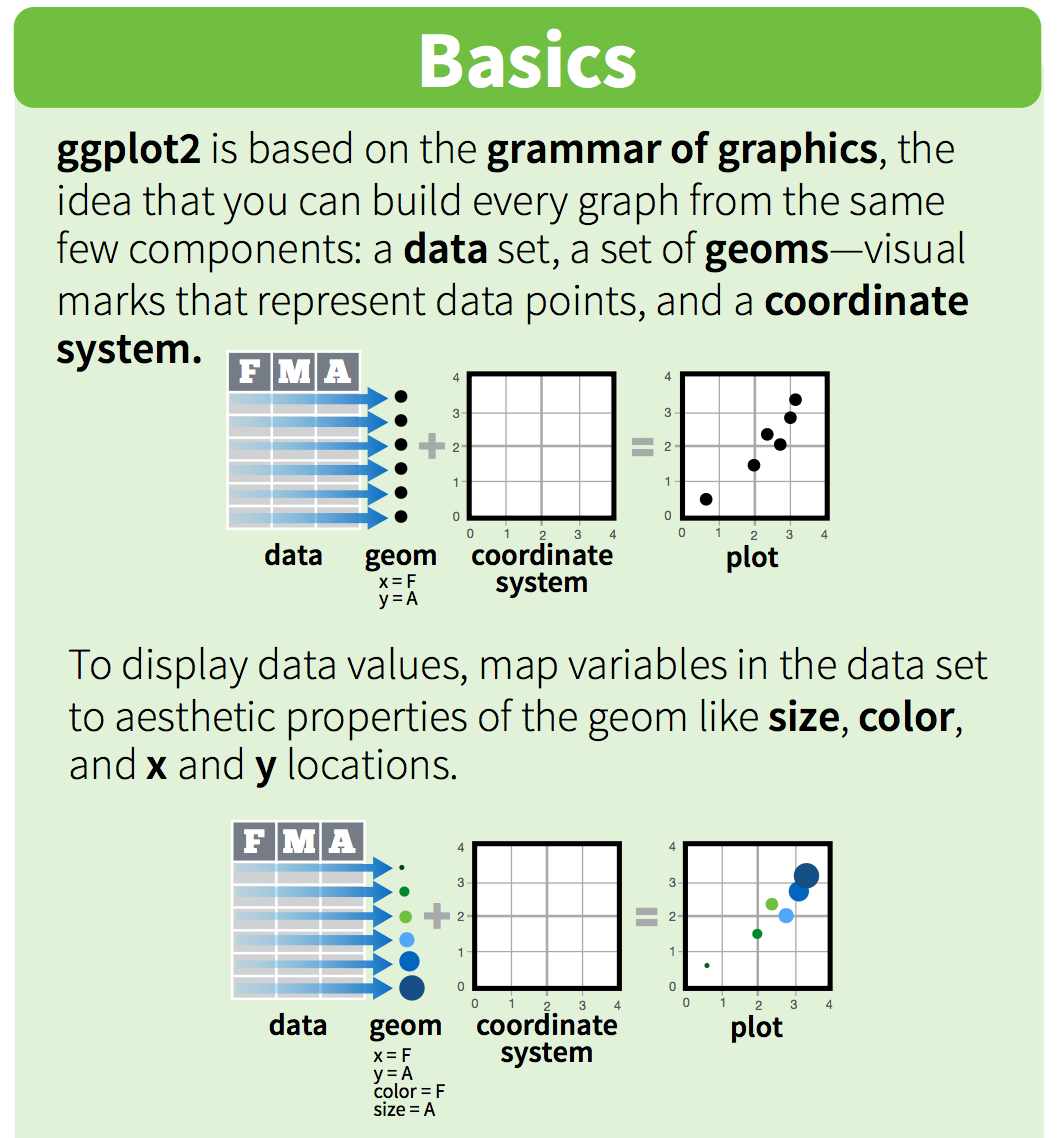
\includegraphics{img/rstudio-cheatsheet-ggplot.png}

\hypertarget{data}{%
\section{Data}\label{data}}

We are going to use a National Park visitation dataset (from the National Park Service at \url{https://irma.nps.gov/Stats/SSRSReports}). Read in the data using \texttt{read\_csv} and take a look at the first few rows using \texttt{head()} or \texttt{View()}.

\begin{Shaded}
\begin{Highlighting}[]
\KeywordTok{head}\NormalTok{(ca)}
\end{Highlighting}
\end{Shaded}

\begin{verbatim}
## # A tibble: 6 x 7
##   region state code  park_name                   type        visitors  year
##   <chr>  <chr> <chr> <chr>                       <chr>          <dbl> <dbl>
## 1 PW     CA    CHIS  Channel Islands National P~ National P~     1200  1963
## 2 PW     CA    CHIS  Channel Islands National P~ National P~     1500  1964
## 3 PW     CA    CHIS  Channel Islands National P~ National P~     1600  1965
## 4 PW     CA    CHIS  Channel Islands National P~ National P~      300  1966
## 5 PW     CA    CHIS  Channel Islands National P~ National P~    15700  1967
## 6 PW     CA    CHIS  Channel Islands National P~ National P~    31000  1968
\end{verbatim}

This dataframe is already in a \emph{long} format where all rows are an observation and all columns are variables. Among the variables in \texttt{ca} are:

\begin{enumerate}
\def\labelenumi{\arabic{enumi}.}
\item
  \texttt{region}, US region where park is located.
\item
  \texttt{visitors}, the annual visitation for each \texttt{year}
\end{enumerate}

To build a ggplot, we need to:

\begin{itemize}
\tightlist
\item
  use the \texttt{ggplot()} function and bind the plot to a specific data frame using the \texttt{data} argument
\end{itemize}

\begin{Shaded}
\begin{Highlighting}[]
\KeywordTok{ggplot}\NormalTok{(}\DataTypeTok{data =}\NormalTok{ ca)}
\end{Highlighting}
\end{Shaded}

\begin{itemize}
\tightlist
\item
  add \texttt{geoms} -- graphical representation of the data in the plot (points,
  lines, bars). \textbf{\texttt{ggplot2}} offers many different geoms; we will use some
  common ones today, including:
  * \texttt{geom\_point()} for scatter plots, dot plots, etc.
  * \texttt{geom\_bar()} for bar charts
  * \texttt{geom\_line()} for trend lines, time-series, etc.
\end{itemize}

To add a geom to the plot use \texttt{+} operator. Because we have two continuous variables,\\
let's use \texttt{geom\_point()} first and then assign x and y aesthetics (\texttt{aes}):

\begin{Shaded}
\begin{Highlighting}[]
\KeywordTok{ggplot}\NormalTok{(}\DataTypeTok{data =}\NormalTok{ ca) }\OperatorTok{+}\StringTok{ }
\StringTok{  }\KeywordTok{geom_point}\NormalTok{(}\KeywordTok{aes}\NormalTok{(}\DataTypeTok{x =}\NormalTok{ year, }\DataTypeTok{y =}\NormalTok{ visitors))}
\end{Highlighting}
\end{Shaded}

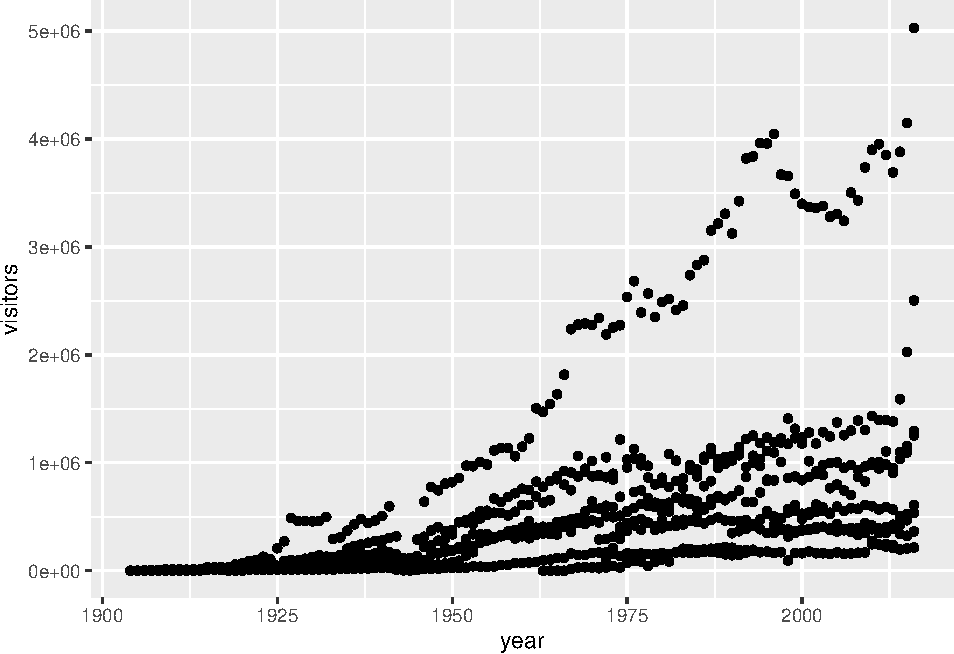
\includegraphics{R_for_Excel_Users_files/figure-latex/first-ggplot-1.pdf}

Notes:

\begin{itemize}
\tightlist
\item
  Anything you put in the \texttt{ggplot()} function can be seen by any geom layers
  that you add (i.e., these are universal plot settings). This includes the x and
  y axis you set up in \texttt{aes()}.
\item
  You can also specify aesthetics for a given geom independently of the
  aesthetics defined globally in the \texttt{ggplot()} function.
\item
  The \texttt{+} sign used to add layers must be placed at the end of each line containing
  a layer. If, instead, the \texttt{+} sign is added in the line before the other layer,
  \textbf{\texttt{ggplot2}} will not add the new layer and will return an error message.
\end{itemize}

\begin{quote}
\textbf{STOP: let's Commit, Pull and Push to GitHub}
\end{quote}

\hypertarget{building-your-plots-iteratively}{%
\section{Building your plots iteratively}\label{building-your-plots-iteratively}}

Building plots with ggplot is typically an iterative process. We start by defining the dataset we'll use, lay the axes, and choose a geom:

\begin{Shaded}
\begin{Highlighting}[]
\KeywordTok{ggplot}\NormalTok{(}\DataTypeTok{data =}\NormalTok{ ca) }\OperatorTok{+}
\StringTok{    }\KeywordTok{geom_point}\NormalTok{(}\KeywordTok{aes}\NormalTok{(}\DataTypeTok{x =}\NormalTok{ year, }\DataTypeTok{y =}\NormalTok{ visitors))}
\end{Highlighting}
\end{Shaded}

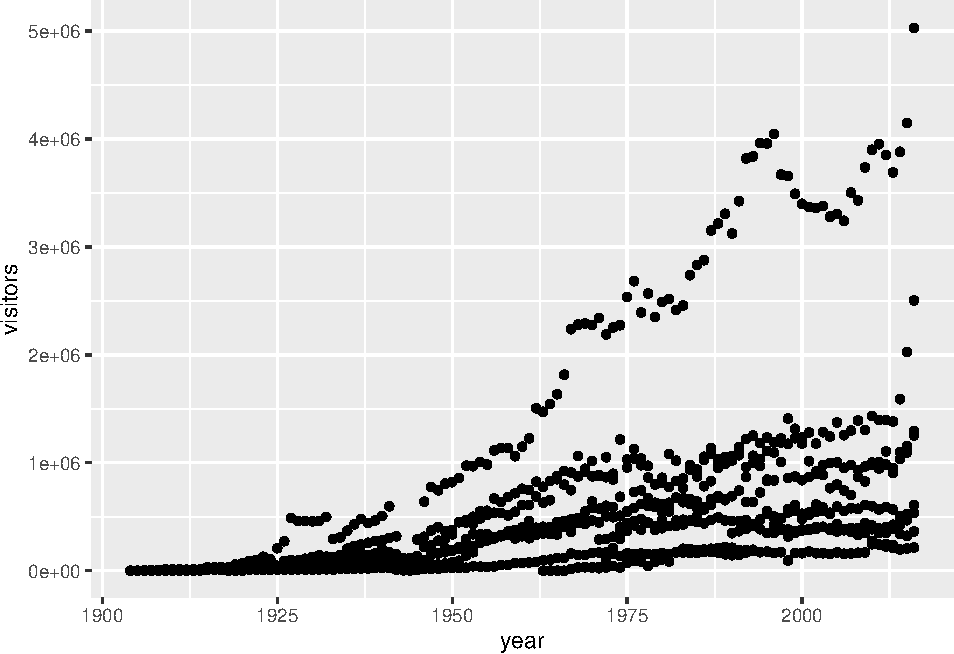
\includegraphics{R_for_Excel_Users_files/figure-latex/create-ggplot-object-1.pdf}

This isn't necessarily a useful way to look at the data. We can distinguish each park by added the \texttt{color} argument to the \texttt{aes}:

\begin{Shaded}
\begin{Highlighting}[]
\KeywordTok{ggplot}\NormalTok{(}\DataTypeTok{data =}\NormalTok{ ca) }\OperatorTok{+}
\StringTok{    }\KeywordTok{geom_point}\NormalTok{(}\KeywordTok{aes}\NormalTok{(}\DataTypeTok{x =}\NormalTok{ year, }\DataTypeTok{y =}\NormalTok{ visitors, }\DataTypeTok{color =}\NormalTok{ park_name))}
\end{Highlighting}
\end{Shaded}

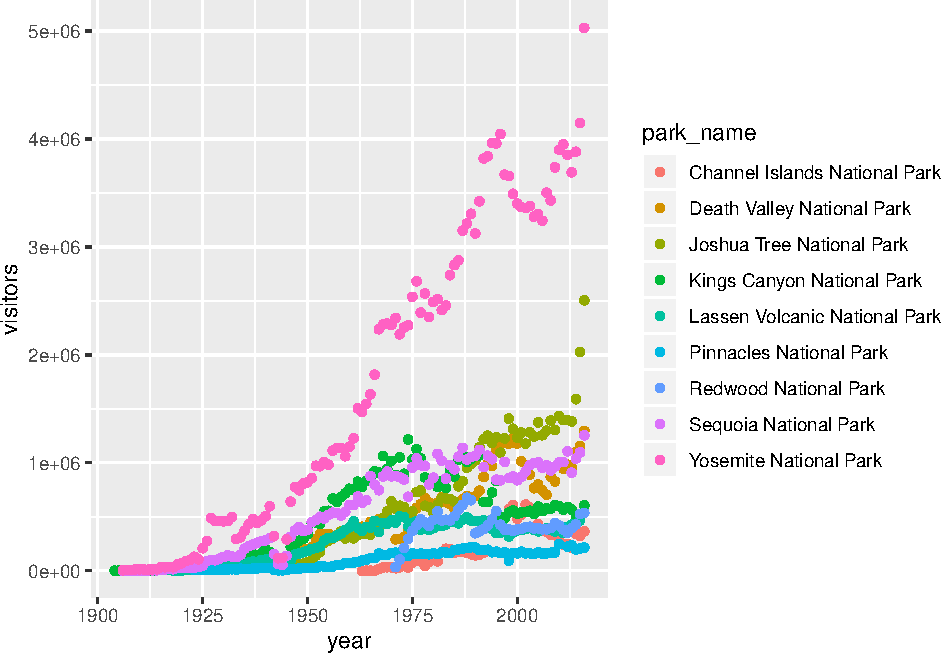
\includegraphics{R_for_Excel_Users_files/figure-latex/color-by-species-1.pdf}

\hypertarget{customizing-plots}{%
\section{Customizing plots}\label{customizing-plots}}

Take a look at the \href{https://www.rstudio.com/wp-content/uploads/2016/11/ggplot2-cheatsheet-2.1.pdf}{\textbf{\texttt{ggplot2}} cheat sheet}, and think of ways you could improve the plot.

Now, let's capitalize the x and y axis labels and add a main title to the figure. I also like to remove that standard gray background using a different \texttt{theme}. Many themes come built into the \texttt{ggplot2} package. My preference is \texttt{theme\_bw()} but once you start typing \texttt{theme\_} a list of options will pop up. The last thing I'm going to do is remove the legend title.

\begin{Shaded}
\begin{Highlighting}[]
\KeywordTok{ggplot}\NormalTok{(}\DataTypeTok{data =}\NormalTok{ ca) }\OperatorTok{+}
\StringTok{    }\KeywordTok{geom_point}\NormalTok{(}\KeywordTok{aes}\NormalTok{(}\DataTypeTok{x =}\NormalTok{ year, }\DataTypeTok{y =}\NormalTok{ visitors, }\DataTypeTok{color =}\NormalTok{ park_name)) }\OperatorTok{+}
\StringTok{    }\KeywordTok{labs}\NormalTok{(}\DataTypeTok{x =} \StringTok{"Year"}\NormalTok{,}
       \DataTypeTok{y =} \StringTok{"Visitation"}\NormalTok{,}
       \DataTypeTok{title =} \StringTok{"California National Park Visitation"}\NormalTok{) }\OperatorTok{+}
\StringTok{    }\KeywordTok{theme_bw}\NormalTok{() }\OperatorTok{+}
\StringTok{    }\KeywordTok{theme}\NormalTok{(}\DataTypeTok{legend.title=}\KeywordTok{element_blank}\NormalTok{())}
\end{Highlighting}
\end{Shaded}

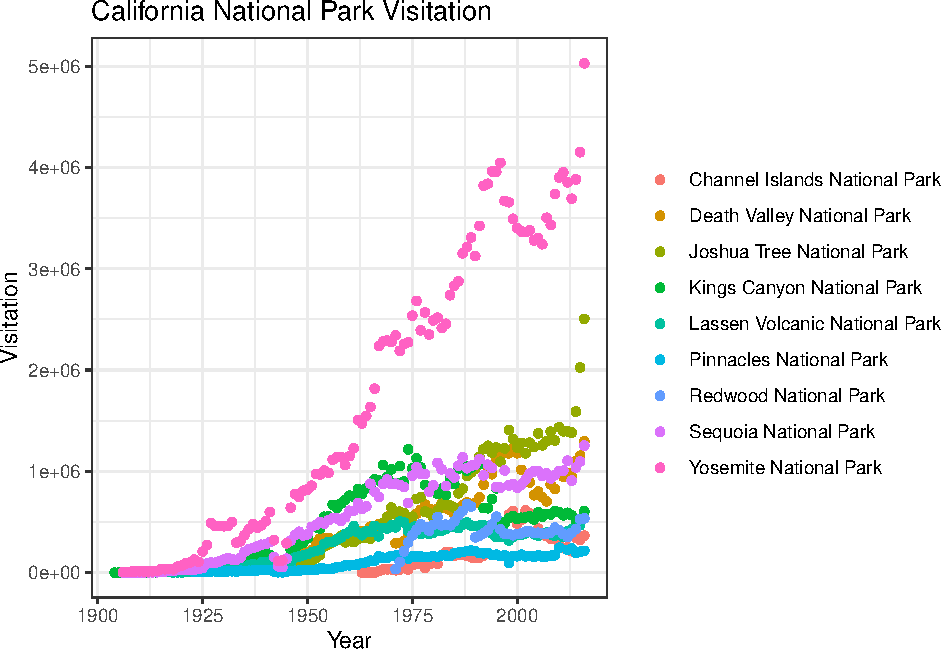
\includegraphics{R_for_Excel_Users_files/figure-latex/customize-1.pdf}

\hypertarget{ggplot2-themes}{%
\section{\texorpdfstring{\textbf{\texttt{ggplot2}} themes}{ggplot2 themes}}\label{ggplot2-themes}}

In addition to \texttt{theme\_bw()}, which changes the plot background to white, \textbf{\texttt{ggplot2}} comes with several other themes which can be useful to quickly change the look of your visualization.

The \href{https://cran.r-project.org/web/packages/ggthemes/vignettes/ggthemes.html}{ggthemes} package provides a wide variety of options (including an Excel 2003 theme). The \href{https://www.ggplot2-exts.org}{\textbf{\texttt{ggplot2}} extensions website} provides a list of packages that extend the capabilities of \textbf{\texttt{ggplot2}}, including additional themes.

\begin{quote}
\hypertarget{exercise-10-min}{%
\subsection{Exercise (10 min)}\label{exercise-10-min}}
\end{quote}

\begin{quote}
\begin{enumerate}
\def\labelenumi{\arabic{enumi}.}
\tightlist
\item
  Using the \texttt{se} dataset, make a scatterplot showing visitation to all national parks in the Southeast region with color identifying individual parks.
\item
  Change the plot so that color indicates \texttt{state}.
\item
  Customize by adding your own title and theme. You can also change the text sizes and angles. Try applying a 45 degree angle to the x-axis. Use your cheatsheet!
\item
  In the code below, why isn't the data showing up?
\end{enumerate}
\end{quote}

\begin{Shaded}
\begin{Highlighting}[]
\KeywordTok{ggplot}\NormalTok{(}\DataTypeTok{data =}\NormalTok{ se, }\KeywordTok{aes}\NormalTok{(}\DataTypeTok{x =}\NormalTok{ year, }\DataTypeTok{y =}\NormalTok{ visitors))}
\end{Highlighting}
\end{Shaded}

\begin{quote}
\mbox{}%
\hypertarget{answers-no-peeking}{%
\paragraph{Answers (no peeking)}\label{answers-no-peeking}}
\end{quote}

\begin{Shaded}
\begin{Highlighting}[]
\CommentTok{# 1.}
\KeywordTok{ggplot}\NormalTok{(}\DataTypeTok{data =}\NormalTok{ se) }\OperatorTok{+}
\StringTok{  }\KeywordTok{geom_point}\NormalTok{(}\KeywordTok{aes}\NormalTok{(}\DataTypeTok{x =}\NormalTok{ year, }\DataTypeTok{y =}\NormalTok{ visitors, }\DataTypeTok{color =}\NormalTok{ park_name))}
\end{Highlighting}
\end{Shaded}

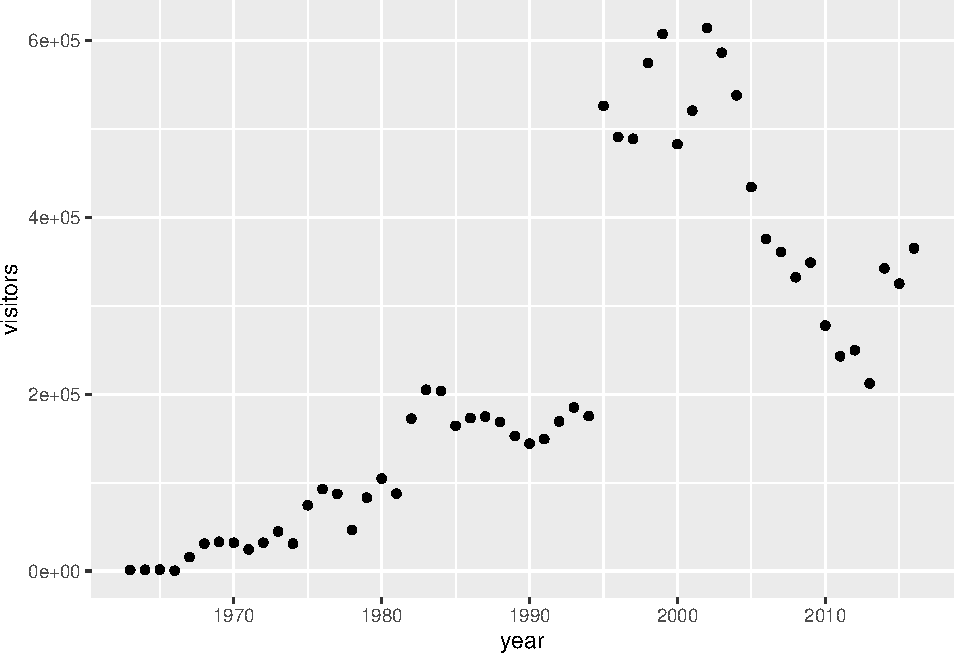
\includegraphics{R_for_Excel_Users_files/figure-latex/unnamed-chunk-53-1.pdf}

\begin{Shaded}
\begin{Highlighting}[]
\CommentTok{# 2. & 3.}
\KeywordTok{ggplot}\NormalTok{(}\DataTypeTok{data =}\NormalTok{ se) }\OperatorTok{+}
\StringTok{  }\KeywordTok{geom_point}\NormalTok{(}\KeywordTok{aes}\NormalTok{(}\DataTypeTok{x =}\NormalTok{ year, }\DataTypeTok{y =}\NormalTok{ visitors, }\DataTypeTok{color =}\NormalTok{ state)) }\OperatorTok{+}
\StringTok{  }\KeywordTok{labs}\NormalTok{(}\DataTypeTok{x =} \StringTok{"Year"}\NormalTok{,}
       \DataTypeTok{y =} \StringTok{"Visitation"}\NormalTok{,}
       \DataTypeTok{title =} \StringTok{"Southeast States National Park Visitation"}\NormalTok{) }\OperatorTok{+}
\StringTok{  }\KeywordTok{theme_light}\NormalTok{() }\OperatorTok{+}
\StringTok{  }\KeywordTok{theme}\NormalTok{(}\DataTypeTok{legend.title =} \KeywordTok{element_blank}\NormalTok{(),}
        \DataTypeTok{axis.text.x =} \KeywordTok{element_text}\NormalTok{(}\DataTypeTok{angle =} \DecValTok{45}\NormalTok{, }\DataTypeTok{hjust =} \DecValTok{1}\NormalTok{, }\DataTypeTok{size =} \DecValTok{14}\NormalTok{))}
\end{Highlighting}
\end{Shaded}

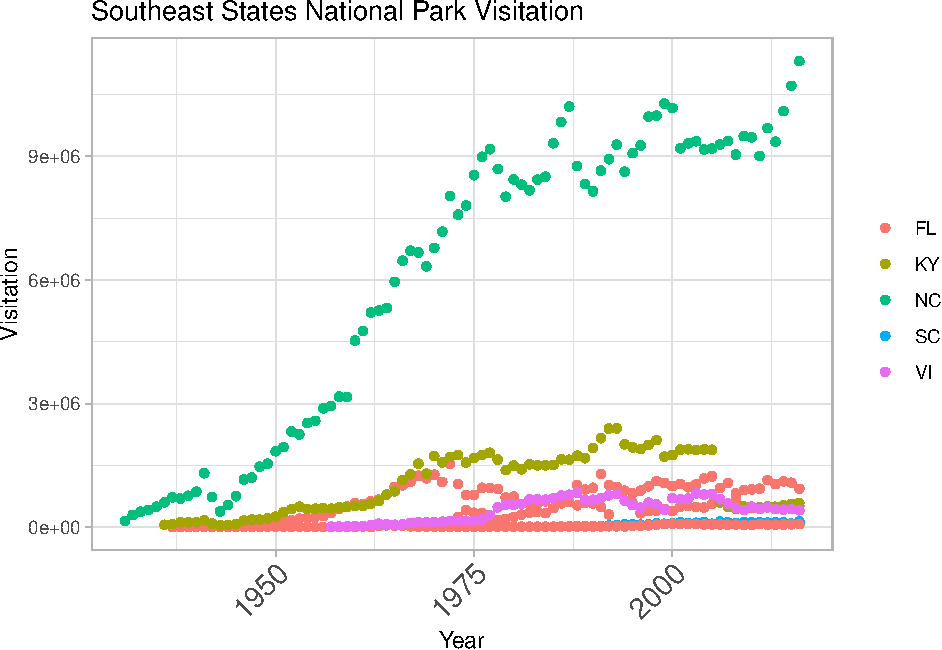
\includegraphics{R_for_Excel_Users_files/figure-latex/unnamed-chunk-53-2.pdf}

\begin{quote}
\begin{enumerate}
\def\labelenumi{\arabic{enumi}.}
\setcounter{enumi}{3}
\tightlist
\item
  The code is missing a geom to describe how the data should be plotted.
\end{enumerate}
\end{quote}

\begin{quote}
\textbf{STOP: commit, pull and push to github}
\end{quote}

\hypertarget{faceting}{%
\section{Faceting}\label{faceting}}

ggplot has a special technique called \emph{faceting} that allows the user to split one plot into multiple plots based on data in the dataset. We will use it to make a plot of park visitation by state:

\begin{Shaded}
\begin{Highlighting}[]
\KeywordTok{ggplot}\NormalTok{(}\DataTypeTok{data =}\NormalTok{ se) }\OperatorTok{+}
\StringTok{    }\KeywordTok{geom_point}\NormalTok{(}\KeywordTok{aes}\NormalTok{(}\DataTypeTok{x =}\NormalTok{ year, }\DataTypeTok{y =}\NormalTok{ visitors)) }\OperatorTok{+}
\StringTok{    }\KeywordTok{facet_wrap}\NormalTok{(}\OperatorTok{~}\StringTok{ }\NormalTok{state)}
\end{Highlighting}
\end{Shaded}

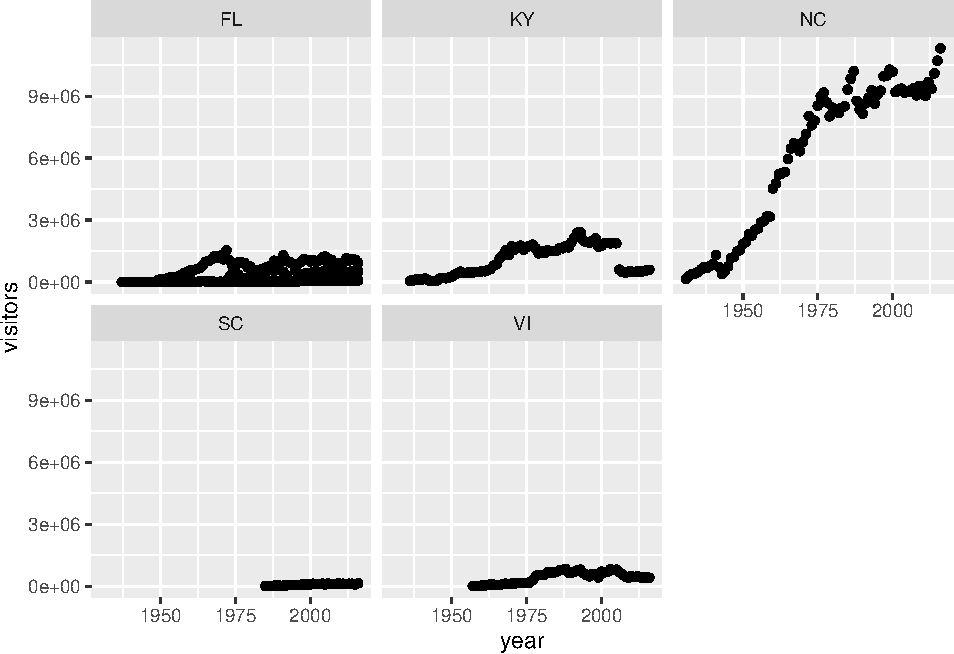
\includegraphics{R_for_Excel_Users_files/figure-latex/first-facet-1.pdf}

We can now make the faceted plot by splitting further by park using \texttt{park\_name} (within a single plot):

\begin{Shaded}
\begin{Highlighting}[]
 \KeywordTok{ggplot}\NormalTok{(}\DataTypeTok{data =}\NormalTok{ se) }\OperatorTok{+}
\StringTok{     }\KeywordTok{geom_point}\NormalTok{(}\KeywordTok{aes}\NormalTok{(}\DataTypeTok{x =}\NormalTok{ year, }\DataTypeTok{y =}\NormalTok{ visitors, }\DataTypeTok{color =}\NormalTok{ park_name)) }\OperatorTok{+}
\StringTok{     }\KeywordTok{facet_wrap}\NormalTok{(}\OperatorTok{~}\StringTok{ }\NormalTok{state, }\DataTypeTok{scales =} \StringTok{"free"}\NormalTok{)}
\end{Highlighting}
\end{Shaded}

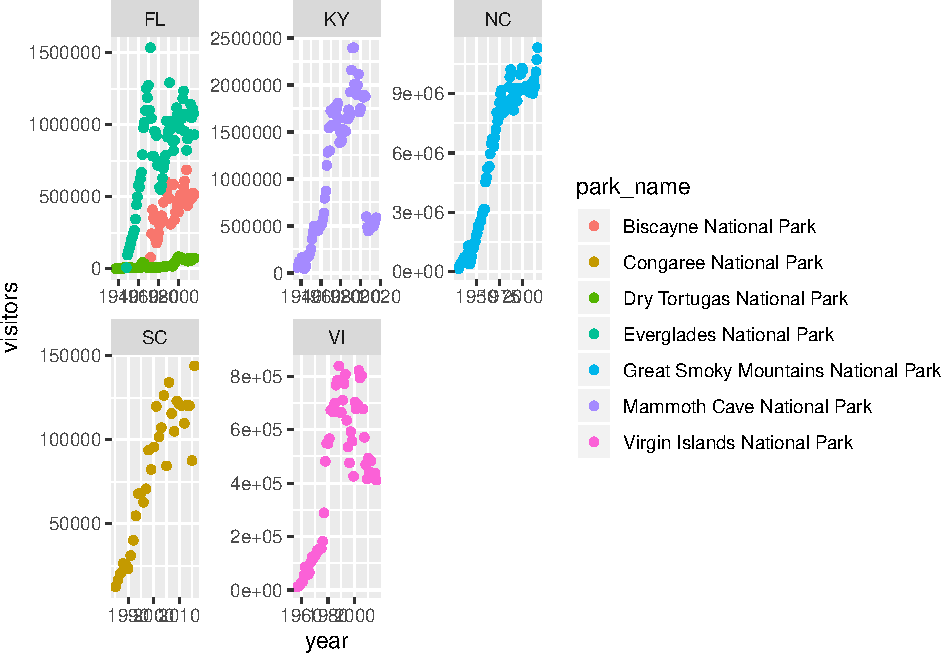
\includegraphics{R_for_Excel_Users_files/figure-latex/facet-by-state-and-park-1.pdf}

\hypertarget{geometric-objects-geoms}{%
\section{Geometric objects (geoms)}\label{geometric-objects-geoms}}

A \textbf{geom} is the geometrical object that a plot uses to represent data. People often describe plots by the type of geom that the plot uses. For example, bar charts use bar geoms, line charts use line geoms, boxplots use boxplot geoms, and so on. Scatterplots break the trend; they use the point geom. You can use different geoms to plot the same data. To change the geom in your plot, change the geom function that you add to \texttt{ggplot()}. Let's look at a few ways of viewing the distribution of annual visitation (\texttt{visitors}) for each park (\texttt{park\_name}).

\begin{Shaded}
\begin{Highlighting}[]
\KeywordTok{ggplot}\NormalTok{(}\DataTypeTok{data =}\NormalTok{ se) }\OperatorTok{+}\StringTok{ }
\StringTok{  }\KeywordTok{geom_jitter}\NormalTok{(}\KeywordTok{aes}\NormalTok{(}\DataTypeTok{x =}\NormalTok{ park_name, }\DataTypeTok{y =}\NormalTok{ visitors, }\DataTypeTok{color =}\NormalTok{ park_name), }
              \DataTypeTok{width =} \FloatTok{0.1}\NormalTok{, }
              \DataTypeTok{alpha =} \FloatTok{0.4}\NormalTok{) }\OperatorTok{+}
\StringTok{  }\KeywordTok{coord_flip}\NormalTok{() }\OperatorTok{+}
\StringTok{  }\KeywordTok{theme}\NormalTok{(}\DataTypeTok{legend.position =} \StringTok{"none"}\NormalTok{) }
\end{Highlighting}
\end{Shaded}

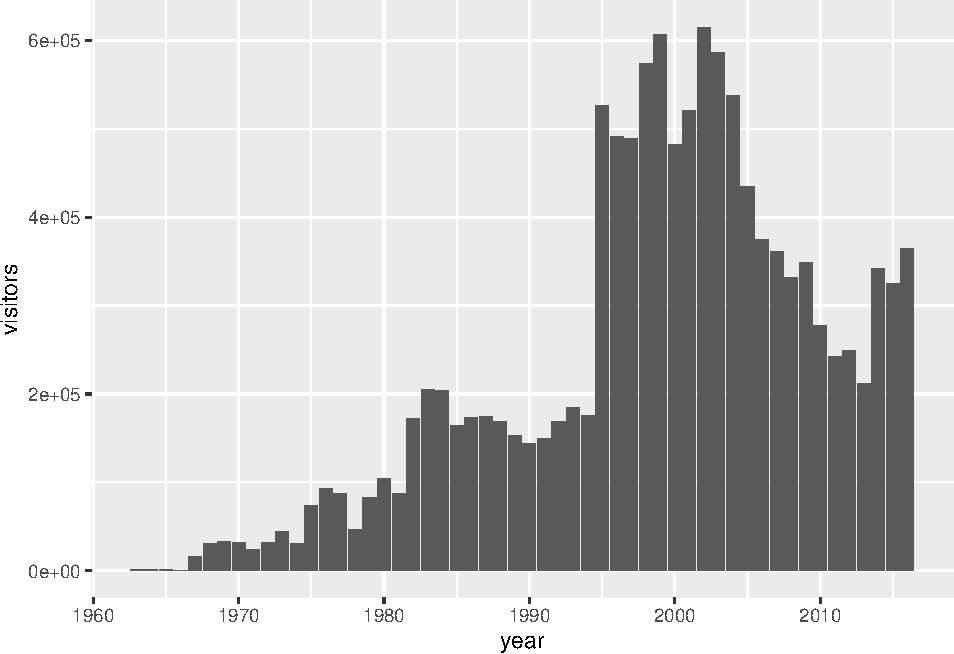
\includegraphics{R_for_Excel_Users_files/figure-latex/unnamed-chunk-54-1.pdf}

\begin{Shaded}
\begin{Highlighting}[]
\KeywordTok{ggplot}\NormalTok{(se, }\KeywordTok{aes}\NormalTok{(}\DataTypeTok{x =}\NormalTok{ park_name, }\DataTypeTok{y =}\NormalTok{ visitors)) }\OperatorTok{+}\StringTok{ }
\StringTok{  }\KeywordTok{geom_boxplot}\NormalTok{() }\OperatorTok{+}
\StringTok{  }\KeywordTok{theme}\NormalTok{(}\DataTypeTok{axis.text.x =} \KeywordTok{element_text}\NormalTok{(}\DataTypeTok{angle =} \DecValTok{45}\NormalTok{, }\DataTypeTok{hjust =} \DecValTok{1}\NormalTok{))}
\end{Highlighting}
\end{Shaded}

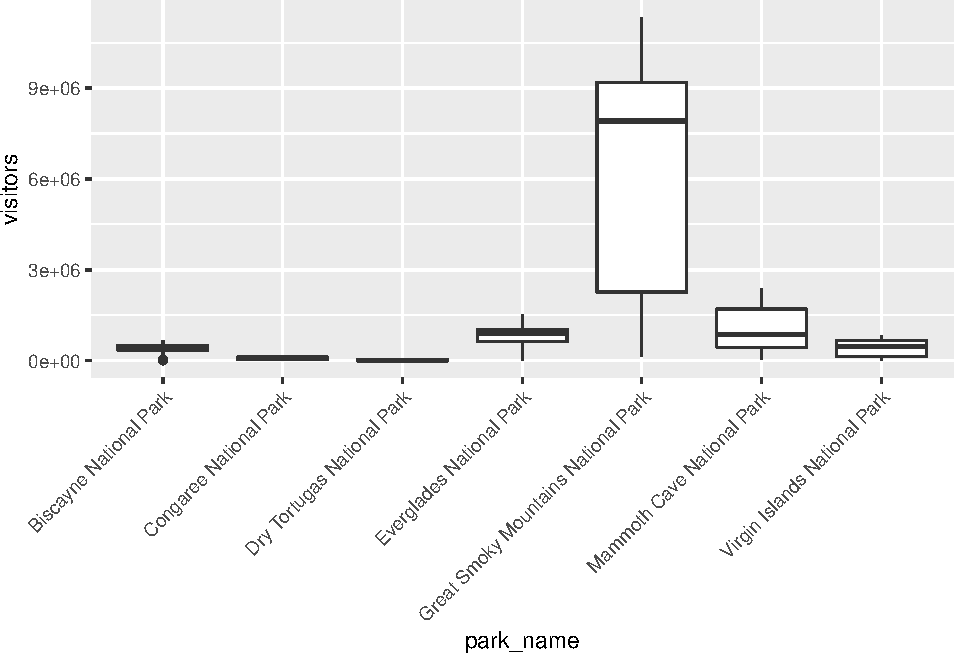
\includegraphics{R_for_Excel_Users_files/figure-latex/unnamed-chunk-54-2.pdf}

None of these are great for visualizing data over time. We can use \texttt{geom\_line()} in the same way we used \texttt{geom\_point}.

\begin{Shaded}
\begin{Highlighting}[]
\KeywordTok{ggplot}\NormalTok{(se, }\KeywordTok{aes}\NormalTok{(}\DataTypeTok{x =}\NormalTok{ year, }\DataTypeTok{y =}\NormalTok{ visitors, }\DataTypeTok{color =}\NormalTok{ park_name)) }\OperatorTok{+}
\StringTok{   }\KeywordTok{geom_line}\NormalTok{()}
\end{Highlighting}
\end{Shaded}

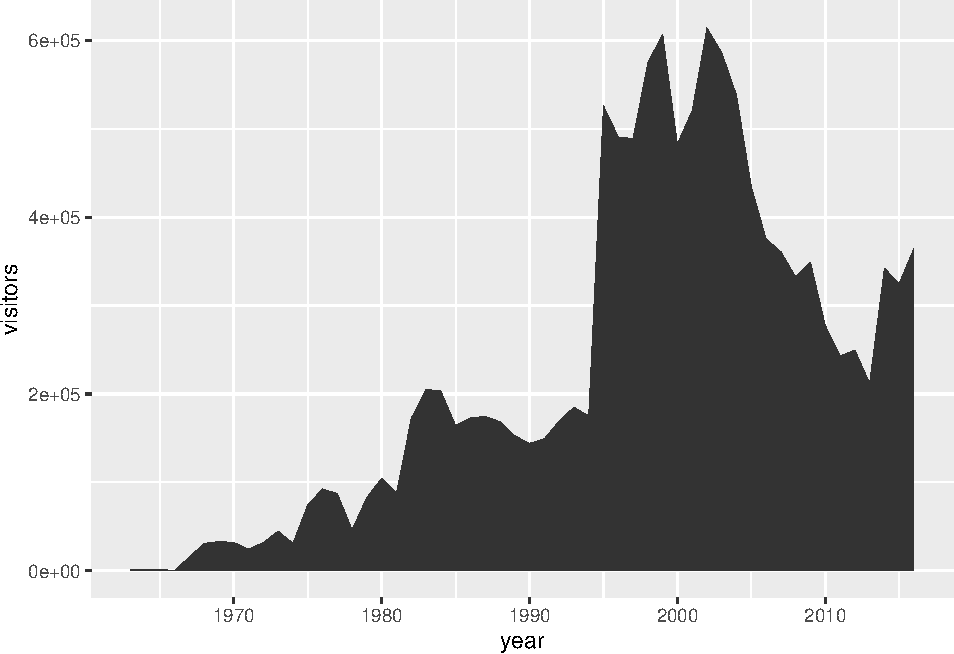
\includegraphics{R_for_Excel_Users_files/figure-latex/unnamed-chunk-55-1.pdf}

\texttt{ggplot2} provides over 30 geoms, and extension packages provide even more (see \url{https://www.ggplot2-exts.org} for a sampling). The best way to get a comprehensive overview is the \href{http://rstudio.com/cheatsheets}{ggplot2 cheatsheet}. To learn more about any single geom, use help: \texttt{?geom\_smooth}.

To display multiple geoms in the same plot, add multiple geom functions to \texttt{ggplot()}:

\texttt{geom\_smooth} allows you to view a smoothed mean of data. Here we look at the smooth mean of visitation over time to Acadia National Park:

\begin{Shaded}
\begin{Highlighting}[]
\KeywordTok{ggplot}\NormalTok{(}\DataTypeTok{data =}\NormalTok{ acadia) }\OperatorTok{+}\StringTok{ }
\StringTok{  }\KeywordTok{geom_point}\NormalTok{(}\KeywordTok{aes}\NormalTok{(}\DataTypeTok{x =}\NormalTok{ year, }\DataTypeTok{y =}\NormalTok{ visitors)) }\OperatorTok{+}
\StringTok{  }\KeywordTok{geom_line}\NormalTok{(}\KeywordTok{aes}\NormalTok{(}\DataTypeTok{x =}\NormalTok{ year, }\DataTypeTok{y =}\NormalTok{ visitors)) }\OperatorTok{+}
\StringTok{  }\KeywordTok{geom_smooth}\NormalTok{(}\KeywordTok{aes}\NormalTok{(}\DataTypeTok{x =}\NormalTok{ year, }\DataTypeTok{y =}\NormalTok{ visitors)) }\OperatorTok{+}
\StringTok{  }\KeywordTok{labs}\NormalTok{(}\DataTypeTok{title =} \StringTok{"Acadia National Park Visitation"}\NormalTok{,}
       \DataTypeTok{y =} \StringTok{"Visitation"}\NormalTok{,}
       \DataTypeTok{x =} \StringTok{"Year"}\NormalTok{) }\OperatorTok{+}
\StringTok{  }\KeywordTok{theme_bw}\NormalTok{()}
\end{Highlighting}
\end{Shaded}

\begin{verbatim}
## `geom_smooth()` using method = 'loess' and formula 'y ~ x'
\end{verbatim}

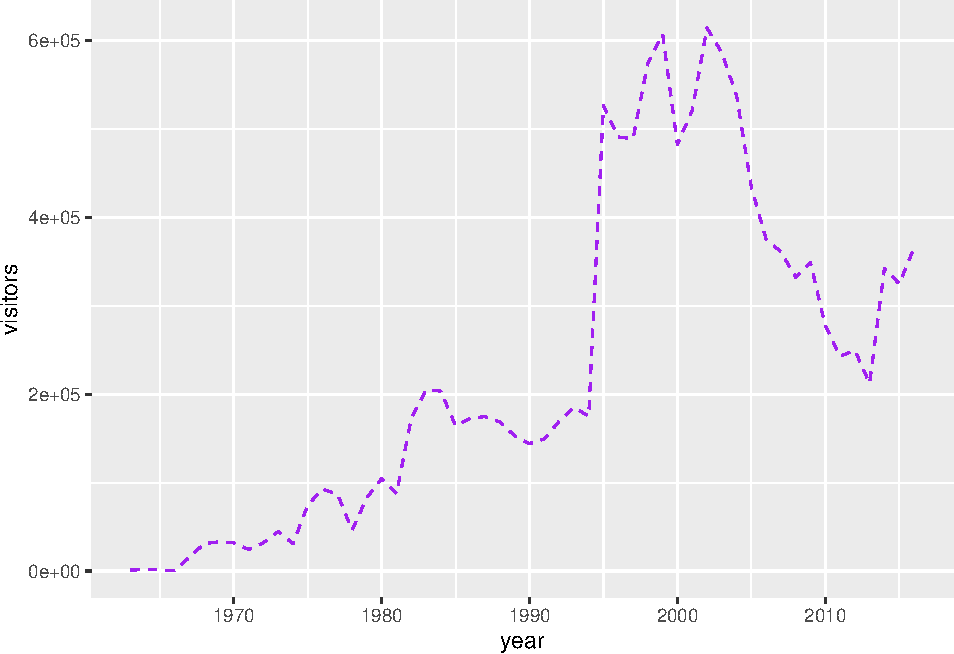
\includegraphics{R_for_Excel_Users_files/figure-latex/unnamed-chunk-56-1.pdf}

Notice that this plot contains three geoms in the same graph! Each geom is using the set of mappings in the first line. ggplot2 will treat these mappings as global mappings that apply to each geom in the graph.

If you place mappings in a geom function, ggplot2 will treat them as local mappings for the layer. It will use these mappings to extend or overwrite the global mappings \emph{for that layer only}. This makes it possible to display different aesthetics in different layers.

\begin{Shaded}
\begin{Highlighting}[]
\KeywordTok{ggplot}\NormalTok{(}\DataTypeTok{data =}\NormalTok{ acadia, }\KeywordTok{aes}\NormalTok{(}\DataTypeTok{x =}\NormalTok{ year, }\DataTypeTok{y =}\NormalTok{ visitors)) }\OperatorTok{+}\StringTok{ }
\StringTok{  }\KeywordTok{geom_point}\NormalTok{() }\OperatorTok{+}
\StringTok{  }\KeywordTok{geom_line}\NormalTok{() }\OperatorTok{+}
\StringTok{  }\KeywordTok{geom_smooth}\NormalTok{(}\DataTypeTok{color =} \StringTok{"red"}\NormalTok{) }\OperatorTok{+}
\StringTok{  }\KeywordTok{labs}\NormalTok{(}\DataTypeTok{title =} \StringTok{"Acadia National Park Visitation"}\NormalTok{,}
       \DataTypeTok{y =} \StringTok{"Visitation"}\NormalTok{,}
       \DataTypeTok{x =} \StringTok{"Year"}\NormalTok{) }\OperatorTok{+}
\StringTok{  }\KeywordTok{theme_bw}\NormalTok{()}
\end{Highlighting}
\end{Shaded}

\begin{verbatim}
## `geom_smooth()` using method = 'loess' and formula 'y ~ x'
\end{verbatim}

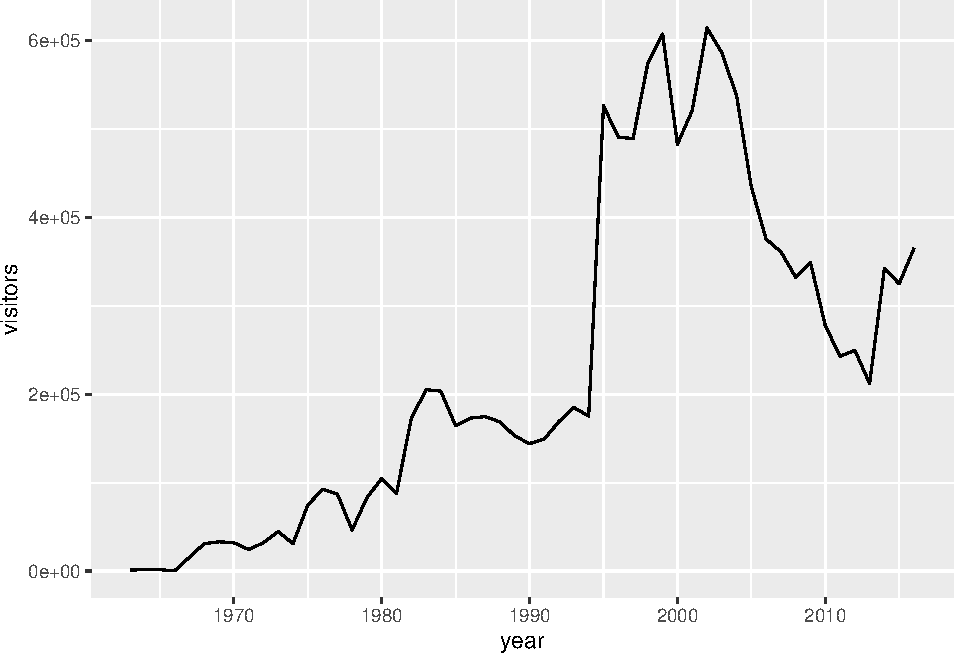
\includegraphics{R_for_Excel_Users_files/figure-latex/unnamed-chunk-57-1.pdf}

\begin{quote}
\hypertarget{challenge}{%
\subsection{Challenge}\label{challenge}}
\end{quote}

\begin{quote}
With all of this information in hand, please take another five minutes to either improve one of the plots generated in this exercise or create a beautiful graph of your own. Use the RStudio \href{https://www.rstudio.com/wp-content/uploads/2016/11/ggplot2-cheatsheet-2.1.pdf}{\textbf{\texttt{ggplot2}} cheat sheet} for inspiration.
\end{quote}

\begin{quote}
Here are some ideas:
\end{quote}

\begin{quote}
\begin{itemize}
\tightlist
\item
  See if you can change the thickness of the lines or line type (e.g.~dashed line).
\item
  Can you find a way to change the name of the legend? What about its labels?
\item
  Try using a different color palette (see \url{http://www.cookbook-r.com/Graphs/Colors_(ggplot2)/}).
\end{itemize}
\end{quote}

\hypertarget{bar-charts}{%
\section{Bar charts}\label{bar-charts}}

Next, let's take a look at a bar chart. Bar charts seem simple, but they are interesting because they reveal something subtle about plots. Consider a basic bar chart, as drawn with \texttt{geom\_bar()}. The following chart displays the total number of parks in each state within the Pacific West region.

\begin{Shaded}
\begin{Highlighting}[]
\KeywordTok{ggplot}\NormalTok{(}\DataTypeTok{data =}\NormalTok{ visit_}\DecValTok{16}\NormalTok{, }\KeywordTok{aes}\NormalTok{(}\DataTypeTok{x =}\NormalTok{ state)) }\OperatorTok{+}\StringTok{ }
\StringTok{  }\KeywordTok{geom_bar}\NormalTok{()}
\end{Highlighting}
\end{Shaded}

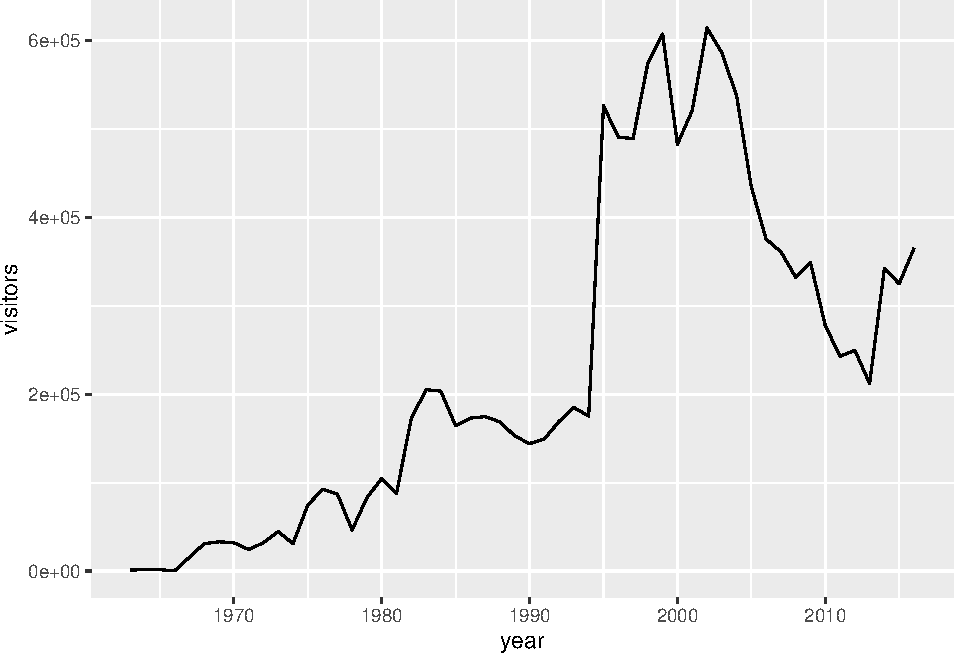
\includegraphics{R_for_Excel_Users_files/figure-latex/unnamed-chunk-58-1.pdf}

On the x-axis, the chart displays \texttt{state}, a variable from \texttt{visit\_16}. On the y-axis, it displays count, but count is not a variable in \texttt{visit\_16}! Where does count come from? Many graphs, like scatterplots, plot the raw values of your dataset. Other graphs, like bar charts, calculate new values to plot:

\begin{itemize}
\item
  bar charts, histograms, and frequency polygons bin your data
  and then plot bin counts, the number of points that fall in each bin.
\item
  smoothers fit a model to your data and then plot predictions from the
  model.
\item
  boxplots compute a robust summary of the distribution and then display a
  specially formatted box.
\end{itemize}

The algorithm used to calculate new values for a graph is called a \textbf{stat}, short for statistical transformation.

You can learn which stat a geom uses by inspecting the default value for the \texttt{stat} argument. For example, \texttt{?geom\_bar} shows that the default value for \texttt{stat} is ``count'', which means that \texttt{geom\_bar()} uses \texttt{stat\_count()}. \texttt{stat\_count()} is documented on the same page as \texttt{geom\_bar()}, and if you scroll down you can find a section called ``Computed variables''. That describes how it computes two new variables: \texttt{count} and \texttt{prop}.

ggplot2 provides over 20 stats for you to use. Each stat is a function, so you can get help in the usual way, e.g. \texttt{?stat\_bin}. To see a complete list of stats, try the ggplot2 cheatsheet.

\hypertarget{position-adjustments}{%
\subsection{Position adjustments}\label{position-adjustments}}

There's one more piece of magic associated with bar charts. You can colour a bar chart using either the \texttt{color} aesthetic, or, more usefully, \texttt{fill}:

\begin{Shaded}
\begin{Highlighting}[]
\KeywordTok{ggplot}\NormalTok{(}\DataTypeTok{data =}\NormalTok{ visit_}\DecValTok{16}\NormalTok{, }\KeywordTok{aes}\NormalTok{(}\DataTypeTok{x =}\NormalTok{ state, }\DataTypeTok{y =}\NormalTok{ visitors, }\DataTypeTok{fill =}\NormalTok{ park_name)) }\OperatorTok{+}\StringTok{ }
\StringTok{  }\KeywordTok{geom_bar}\NormalTok{(}\DataTypeTok{stat =} \StringTok{"identity"}\NormalTok{)}
\end{Highlighting}
\end{Shaded}

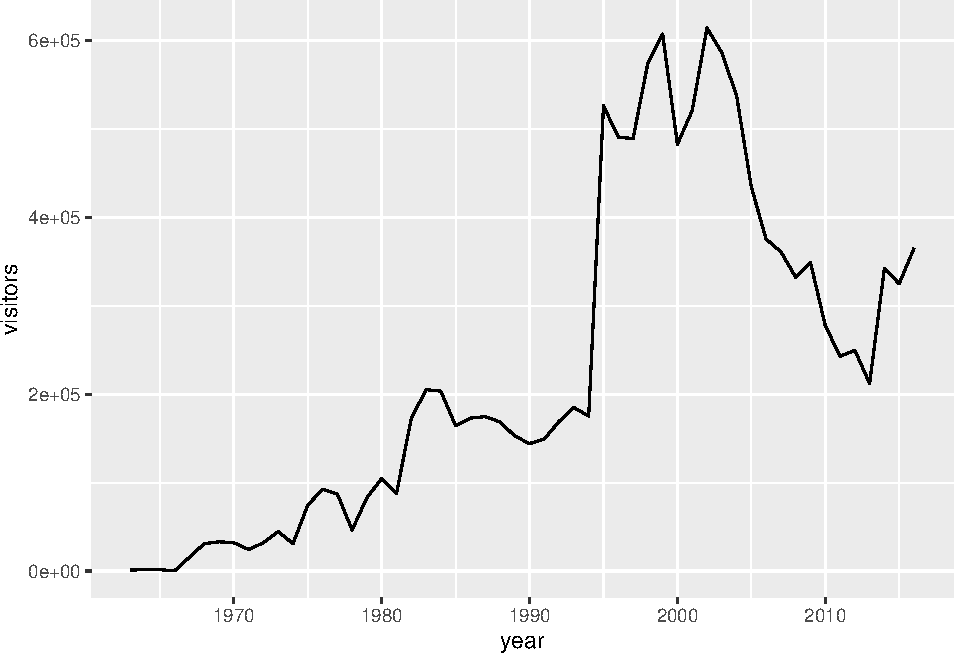
\includegraphics{R_for_Excel_Users_files/figure-latex/unnamed-chunk-59-1.pdf}

The stacking is performed automatically by the \textbf{position adjustment} specified by the \texttt{position} argument. If you don't want a stacked bar chart, you can use \texttt{"dodge"}.

\begin{itemize}
\tightlist
\item
  \texttt{position\ =\ "dodge"} places overlapping objects directly \emph{beside} one
  another. This makes it easier to compare individual values.
\end{itemize}

\begin{Shaded}
\begin{Highlighting}[]
\KeywordTok{ggplot}\NormalTok{(}\DataTypeTok{data =}\NormalTok{ visit_}\DecValTok{16}\NormalTok{, }\KeywordTok{aes}\NormalTok{(}\DataTypeTok{x =}\NormalTok{ state, }\DataTypeTok{y =}\NormalTok{ visitors, }\DataTypeTok{fill =}\NormalTok{ park_name)) }\OperatorTok{+}\StringTok{ }
\StringTok{  }\KeywordTok{geom_bar}\NormalTok{(}\DataTypeTok{stat =} \StringTok{"identity"}\NormalTok{, }\DataTypeTok{position =} \StringTok{"dodge"}\NormalTok{)}
\end{Highlighting}
\end{Shaded}

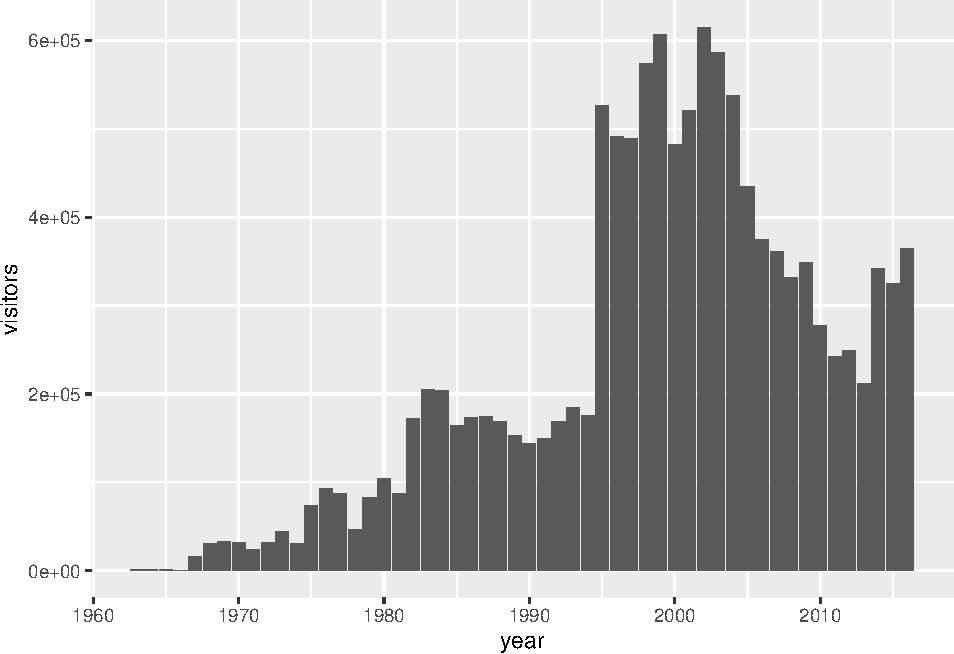
\includegraphics{R_for_Excel_Users_files/figure-latex/unnamed-chunk-60-1.pdf}

\hypertarget{challenge-1}{%
\subsection{Challenge}\label{challenge-1}}

\begin{quote}
With all of this information in hand, please take another five minutes to either
improve one of the plots generated in this exercise or create a beautiful graph
of your own. Use the RStudio \href{https://www.rstudio.com/wp-content/uploads/2016/11/ggplot2-cheatsheet-2.1.pdf}{\textbf{\texttt{ggplot2}} cheat sheet} for
inspiration. Remember to use the help documentation (e.g. \texttt{?geom\_bar})
\end{quote}

\begin{quote}
Here are some ideas:
\end{quote}

\begin{quote}
\begin{itemize}
\tightlist
\item
  Flip the x and y axes.
\item
  Change the color palette used
\item
  Use \texttt{scale\_x\_discrete} to change the x-axis tick labels to the full state names (Arizona, Colorado, etc.)
\item
  Make a bar chart using the Massachussets dataset (\texttt{mass}) and find out how many parks of each type are in the state.
\end{itemize}
\end{quote}

\hypertarget{answers-no-peeking-1}{%
\paragraph{Answers (no peeking!)}\label{answers-no-peeking-1}}

\begin{Shaded}
\begin{Highlighting}[]
\CommentTok{#how many of each types of parks are in Massachusetts?}
\KeywordTok{ggplot}\NormalTok{(}\DataTypeTok{data =}\NormalTok{ mass) }\OperatorTok{+}\StringTok{ }
\StringTok{      }\KeywordTok{geom_bar}\NormalTok{(}\KeywordTok{aes}\NormalTok{(}\DataTypeTok{x =}\NormalTok{ type, }\DataTypeTok{fill =}\NormalTok{ park_name)) }\OperatorTok{+}
\StringTok{  }\KeywordTok{labs}\NormalTok{(}\DataTypeTok{x =} \StringTok{""}\NormalTok{,}
       \DataTypeTok{y =} \StringTok{""}\NormalTok{)}\OperatorTok{+}
\StringTok{  }\KeywordTok{theme}\NormalTok{(}\DataTypeTok{axis.text.x =} \KeywordTok{element_text}\NormalTok{(}\DataTypeTok{angle =} \DecValTok{45}\NormalTok{, }\DataTypeTok{hjust =} \DecValTok{1}\NormalTok{, }\DataTypeTok{size =} \DecValTok{7}\NormalTok{))}
\end{Highlighting}
\end{Shaded}

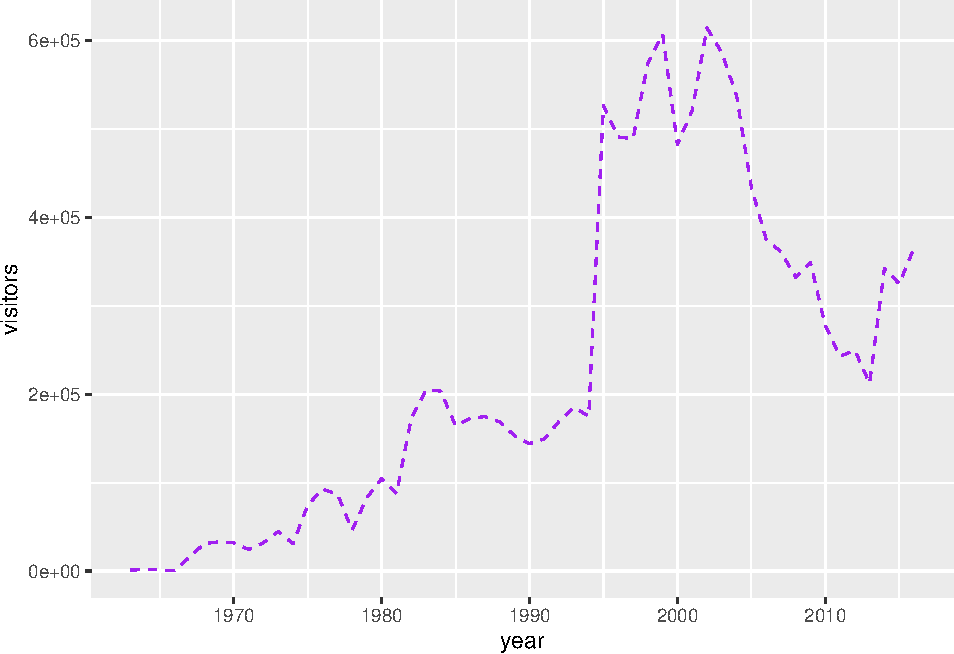
\includegraphics{R_for_Excel_Users_files/figure-latex/unnamed-chunk-61-1.pdf}

\hypertarget{arranging-and-exporting-plots}{%
\section{Arranging and exporting plots}\label{arranging-and-exporting-plots}}

After creating your plot, you can save it to a file in your favorite format. The Export tab in the \textbf{Plot} pane in RStudio will save your plots at low resolution, which will not be accepted by many journals and will not scale well for posters.

Instead, use the \texttt{ggsave()} function, which allows you easily change the dimension and resolution of your plot by adjusting the appropriate arguments (\texttt{width}, \texttt{height} and \texttt{dpi}):

\begin{Shaded}
\begin{Highlighting}[]
\NormalTok{my_plot <-}\StringTok{ }\KeywordTok{ggplot}\NormalTok{(}\DataTypeTok{data =}\NormalTok{ mass) }\OperatorTok{+}\StringTok{ }
\StringTok{      }\KeywordTok{geom_bar}\NormalTok{(}\KeywordTok{aes}\NormalTok{(}\DataTypeTok{x =}\NormalTok{ type, }\DataTypeTok{fill =}\NormalTok{ park_name)) }\OperatorTok{+}
\StringTok{  }\KeywordTok{labs}\NormalTok{(}\DataTypeTok{x =} \StringTok{""}\NormalTok{,}
       \DataTypeTok{y =} \StringTok{""}\NormalTok{)}\OperatorTok{+}
\StringTok{  }\KeywordTok{theme}\NormalTok{(}\DataTypeTok{axis.text.x =} \KeywordTok{element_text}\NormalTok{(}\DataTypeTok{angle =} \DecValTok{45}\NormalTok{, }\DataTypeTok{hjust =} \DecValTok{1}\NormalTok{, }\DataTypeTok{size =} \DecValTok{7}\NormalTok{))}

\KeywordTok{ggsave}\NormalTok{(}\StringTok{"name_of_file.png"}\NormalTok{, my_plot, }\DataTypeTok{width =} \DecValTok{15}\NormalTok{, }\DataTypeTok{height =} \DecValTok{10}\NormalTok{)}
\end{Highlighting}
\end{Shaded}

Note: The parameters \texttt{width} and \texttt{height} also determine the font size in the saved plot.

\hypertarget{bonus}{%
\section{Bonus}\label{bonus}}

So as you can see, \texttt{ggplot2} is a fantastic package for visualizing data. But there are some additional packages that let you make plots interactive. \texttt{plotly}, \texttt{gganimate}.

\begin{Shaded}
\begin{Highlighting}[]
\CommentTok{#install.packages("plotly")}
\KeywordTok{library}\NormalTok{(plotly)}

\KeywordTok{ggplotly}\NormalTok{(my_plot)}
\end{Highlighting}
\end{Shaded}

\begin{Shaded}
\begin{Highlighting}[]
\NormalTok{acad_vis <-}\StringTok{ }\KeywordTok{ggplot}\NormalTok{(}\DataTypeTok{data =}\NormalTok{ acadia, }\KeywordTok{aes}\NormalTok{(}\DataTypeTok{x =}\NormalTok{ year, }\DataTypeTok{y =}\NormalTok{ visitors)) }\OperatorTok{+}\StringTok{ }
\StringTok{  }\KeywordTok{geom_point}\NormalTok{() }\OperatorTok{+}
\StringTok{  }\KeywordTok{geom_line}\NormalTok{() }\OperatorTok{+}
\StringTok{  }\KeywordTok{geom_smooth}\NormalTok{(}\DataTypeTok{color =} \StringTok{"red"}\NormalTok{) }\OperatorTok{+}
\StringTok{  }\KeywordTok{labs}\NormalTok{(}\DataTypeTok{title =} \StringTok{"Acadia National Park Visitation"}\NormalTok{,}
       \DataTypeTok{y =} \StringTok{"Visitation"}\NormalTok{,}
       \DataTypeTok{x =} \StringTok{"Year"}\NormalTok{) }\OperatorTok{+}
\StringTok{  }\KeywordTok{theme_bw}\NormalTok{()}

\KeywordTok{ggplotly}\NormalTok{(acad_vis)}
\end{Highlighting}
\end{Shaded}

\hypertarget{save-and-push-to-github}{%
\section{Save and push to GitHub}\label{save-and-push-to-github}}

\hypertarget{fun-facts-quirky-things---making-a-note-of-these-wherever-possible-for-interest-little-did-you-know-sections-2}{%
\section{Fun facts (quirky things) - making a note of these wherever possible for interest (little ``Did you know?'' sections)}\label{fun-facts-quirky-things---making-a-note-of-these-wherever-possible-for-interest-little-did-you-know-sections-2}}

\hypertarget{interludes-deep-thoughtsopenscapes-4}{%
\section{Interludes (deep thoughts/openscapes)}\label{interludes-deep-thoughtsopenscapes-4}}

\hypertarget{our-turn-your-turn-1-1}{%
\section{Our Turn Your Turn 1}\label{our-turn-your-turn-1-1}}

\hypertarget{our-turn-your-turn-2-1}{%
\section{Our Turn Your Turn 2}\label{our-turn-your-turn-2-1}}

\hypertarget{efficiency-tips-4}{%
\section{Efficiency Tips}\label{efficiency-tips-4}}

\hypertarget{pivot}{%
\chapter{\texorpdfstring{\texttt{dplyr} and Pivot Tables}{dplyr and Pivot Tables}}\label{pivot}}

TODO:
use lobster data.
Start with counted data and show uncount and discuss why it's important to have counted data
Count and uncount, summary statistics
Use uncounted lobster data
summarize(mean, sd, n) with uncounted lobster data (stdev in excel?)
DT, kable --- introduce this and then will be repeated in tidying
if time, could we show count vs n but if you want to get other statistics

TODO:
Explore data:
summaries/data table
Uncount and count
Why would you ever want to uncount? You don't want to assume how future you will want to use this data
How easy is it to get these counts by different groupings
Simplest ggplot (introduced in readxl chapter)

\hypertarget{summary-a-few-sentences}{%
\section{Summary (a few sentences)}\label{summary-a-few-sentences}}

We will learn how to wrangle data in R, using the \texttt{dplyr} package which is included in the \texttt{tidyverse}. package. In this session, we'll focus on the functions in \texttt{dplyr} that operate like Excel's pivot tables.

\hypertarget{objectives-more-detailed-bulletpoints-2}{%
\section{Objectives (more detailed, bulletpoints?)}\label{objectives-more-detailed-bulletpoints-2}}

In R, we can use dplyr for pivot tables by using 2 main verbs in combination: \texttt{group\_by} and \texttt{summarize}, and that's where we'll start. Then, we will learn 2 critical verbs that are powerful for data wrangling: \texttt{mutate} and \texttt{select}.

We will also continue to emphasize reproducibility in all our analyses.

\begin{itemize}
\tightlist
\item
  Practice our reproducible workflow with RMarkdown and GitHub
\item
  Discuss pivot tables in Excel
\item
  Introduce the \texttt{dplyr} package in R
\end{itemize}

\hypertarget{resources-5}{%
\section{Resources}\label{resources-5}}

\begin{itemize}
\tightlist
\item
  \href{https://dplyr.tidyverse.org/}{dplyr.tidyverse.org}
\item
  \href{https://r4ds.had.co.nz/transform.html}{R for Data Science: Transform Chapter}
\item
  \href{https://youtu.be/g530cnFfk8Y}{Intro to Pivot Tables I-III} by Excel Campus
\end{itemize}

\hypertarget{lesson-1}{%
\section{Lesson}\label{lesson-1}}

TODO
We've talked about

\hypertarget{setup}{%
\subsection{Setup}\label{setup}}

Let's start a new RMarkdown file, called X.

In the setup chunk, let's attach our libraries and read in the lobster counts data.

\begin{Shaded}
\begin{Highlighting}[]
\CommentTok{## attach libraries}
\KeywordTok{library}\NormalTok{(tidyverse)}

\CommentTok{## read in data}
\NormalTok{lobster_counts <-}\StringTok{ }\KeywordTok{read_csv}\NormalTok{(}\StringTok{"lobster_counts_curated.csv"}\NormalTok{)}
\end{Highlighting}
\end{Shaded}

Let's add a code chunk to explore the data by looking at some summary statistics and making a simple plot.

\begin{Shaded}
\begin{Highlighting}[]
\CommentTok{#TODO}
\KeywordTok{head}\NormalTok{(lobster_counts) }\CommentTok{# year and month as well as a column for date}
\end{Highlighting}
\end{Shaded}

\begin{verbatim}
## # A tibble: 6 x 10
##    year month date    site  transect replicate size_mm count num_ao  area
##   <dbl> <dbl> <chr>   <chr>    <dbl> <chr>       <dbl> <dbl>  <dbl> <dbl>
## 1  2012     8 8/20/12 ivee         1 A              NA     0      0   300
## 2  2012     8 8/20/12 ivee         1 B              NA     0      0   300
## 3  2012     8 8/20/12 ivee         1 C              NA     0      0   300
## 4  2012     8 8/20/12 ivee         1 D              NA     0      0   300
## 5  2012     8 8/20/12 ivee         2 A              NA     0      0   300
## 6  2012     8 8/20/12 ivee         2 B              NA     0      0   300
\end{verbatim}

\begin{Shaded}
\begin{Highlighting}[]
\KeywordTok{summary}\NormalTok{(lobster_counts)}
\end{Highlighting}
\end{Shaded}

\begin{verbatim}
##       year          month           date               site          
##  Min.   :2012   Min.   :8.000   Length:4362        Length:4362       
##  1st Qu.:2015   1st Qu.:8.000   Class :character   Class :character  
##  Median :2016   Median :8.000   Mode  :character   Mode  :character  
##  Mean   :2016   Mean   :8.018                                        
##  3rd Qu.:2018   3rd Qu.:8.000                                        
##  Max.   :2018   Max.   :9.000                                        
##                                                                      
##     transect      replicate            size_mm           count       
##  Min.   :1.000   Length:4362        Min.   : 18.00   Min.   : 0.000  
##  1st Qu.:2.000   Class :character   1st Qu.: 65.00   1st Qu.: 1.000  
##  Median :4.000   Mode  :character   Median : 75.00   Median : 1.000  
##  Mean   :4.056                      Mean   : 74.45   Mean   : 1.459  
##  3rd Qu.:6.000                      3rd Qu.: 84.00   3rd Qu.: 2.000  
##  Max.   :9.000                      Max.   :183.00   Max.   :41.000  
##                                     NA's   :350                      
##      num_ao              area    
##  Min.   : 0.00000   Min.   :300  
##  1st Qu.: 0.00000   1st Qu.:300  
##  Median : 0.00000   Median :300  
##  Mean   : 0.04104   Mean   :300  
##  3rd Qu.: 0.00000   3rd Qu.:300  
##  Max.   :10.00000   Max.   :300  
## 
\end{verbatim}

\begin{Shaded}
\begin{Highlighting}[]
\CommentTok{# summary, head, tail, depending on readxl}
\CommentTok{# ggplot}
\end{Highlighting}
\end{Shaded}

Also explore in the Viewer

OK now let's step back from R and discuss pivot tables in Excel.

\hypertarget{pivot-tables}{%
\subsection{Pivot tables}\label{pivot-tables}}

\hypertarget{what-are-they}{%
\subsubsection{What are they?}\label{what-are-they}}

TODO: screenshots, demo with lobster data.

What is actually going on is that they are summarizing by the groups you identify.

So I'm looking at my lobster data in Excel and I really want to know how many lobsters were counted at each site. I want a summary of total counts by site. So to do this in Excel we would initiate the Pivot Table Process:

And it will do its best to find the data I would like to include in my Pivot Table (it can have difficulty with non-rectangular or ``non-tidy'' data), and suggest we make this in a new sheet:

And then we'll get a little wizard to help us create the Pivot Table. I want to summarize by site, so I drag ``site'' down into the ``Rows'' box, and then I drag ``count'' into the ``Values'' box. And it will create a Pivot Table for me, with ``sum'' as the default summary statistic.

A few things to note:

\begin{itemize}
\tightlist
\item
  The pivot table is separate entity from our data (it's on a different sheet); the original data has not been affected
\item
  The pivot table only shows the variables we requested; we don't see other columns (like date, month, or site).
\end{itemize}

\hypertarget{why-are-they-great}{%
\subsubsection{Why are they great?}\label{why-are-they-great}}

Pivot tables are great because they summarize the data and keep the raw data raw --- they even promote good pratice because they by default ask you if you'd like to present the data in a new sheet rather than in the same sheet.

If you add new data, you can refresh your table

\hypertarget{why-would-we-want-to-work-in-r-instead}{%
\subsubsection{Why would we want to work in R instead?}\label{why-would-we-want-to-work-in-r-instead}}

Let's talk about how this looks like in R.

\hypertarget{dplyr-overview}{%
\section{\texorpdfstring{\texttt{dplyr} overview}{dplyr overview}}\label{dplyr-overview}}

\texttt{dplyr} is a grammar of data manipulation that provides a consistent set of verbs that help you solve the most common data manipulation challenges. These common verbs are:

\begin{itemize}
\item
  \textbf{\texttt{filter()}}: pick observations by their values
\item
  \textbf{\texttt{select()}}: pick variables by their names
\item
  \textbf{\texttt{mutate()}}: create new variables with functions of existing variables
\item
  \textbf{\texttt{summarise()}}: collapse many values down to a single summary
\item
  \textbf{\texttt{arrange()}}: reorder the rows
\end{itemize}

These can all be used in conjunction with \texttt{group\_by()} which changes the scope of each function from operating on the entire dataset to operating on it group-by-group. These six functions provide the verbs for a language of data manipulation.

All verbs work similarly:

\begin{enumerate}
\def\labelenumi{\arabic{enumi}.}
\tightlist
\item
  The first argument is a data frame.
\item
  The subsequent arguments describe what to do with the data frame. You can refer to columns in the data frame directly without using \texttt{\$}.
\item
  The result is a new data frame.
\end{enumerate}

Together these properties make it easy to chain together multiple simple steps to achieve a complex result using the pipe operator \texttt{\%\textgreater{}\%}.

I love thinking of these \texttt{dplyr} verbs and the pipe operator \texttt{\%\textgreater{}\%} as telling a story. When I see \texttt{\%\textgreater{}\%} I think ``and then'':

\begin{Shaded}
\begin{Highlighting}[]
\NormalTok{data }\OperatorTok\StringTok{          }\CommentTok{# start with data, and then}
\StringTok{  }\KeywordTok{group_by}\NormalTok{() }\OperatorTok\StringTok{  }\CommentTok{# group by a variable, and then}
\StringTok{  }\KeywordTok{mutate}\NormalTok{() }\OperatorTok\StringTok{    }\CommentTok{# mutate to add a new column, and then}
\StringTok{  }\KeywordTok{select}\NormalTok{()        }\CommentTok{# select specific columns}
\end{Highlighting}
\end{Shaded}

\hypertarget{group_by-summarize}{%
\section{group\_by() \%\textgreater{}\% summarize()}\label{group_by-summarize}}

In R, we can create the functionality of pivot tables by using 2 main \texttt{dplyr} verbs in combination: \texttt{group\_by} and \texttt{summarize}.

Say it with me: ``pivot tables are group\_by and then summarize''. And just like pivot tables, you have flexibility with how you are going to summarize. For example, we can calculate an average, or a total.

\hypertarget{group_by-one-variable}{%
\subsection{group\_by one variable}\label{group_by-one-variable}}

Let's try this on our \texttt{lobster\_counts} data. Let's calculate the the total number of lobster by year. In R-speak, we will group\_by year and then summarize by calculting the sum of count. We'll use the pipe operator \texttt{\%\textgreater{}\%}

\begin{Shaded}
\begin{Highlighting}[]
\NormalTok{lobster_counts }\OperatorTok
\StringTok{  }\KeywordTok{group_by}\NormalTok{(year) }\OperatorTok
\StringTok{  }\KeywordTok{summarize}\NormalTok{(}\DataTypeTok{total_lobster =} \KeywordTok{sum}\NormalTok{(count)) }\CommentTok{# within summarize, we name a new column and calculate the sum.}
\end{Highlighting}
\end{Shaded}

\begin{verbatim}
## # A tibble: 7 x 2
##    year total_lobster
##   <dbl>         <dbl>
## 1  2012           231
## 2  2013           243
## 3  2014           510
## 4  2015          1100
## 5  2016           809
## 6  2017          1668
## 7  2018          1805
\end{verbatim}

This returns output summarizing the total\_lobster for each year, just like we saw in the pivot table in Excel.

Notice how together, \texttt{group\_by} and \texttt{summarize} minimize the amount of information we see. We also saw this with the pivot table. We lose the other columns that aren't involved here.

Question: What if you \emph{don't} group\_by first? Let's try it and discuss what's going on.

\begin{Shaded}
\begin{Highlighting}[]
\NormalTok{lobster_counts }\OperatorTok
\StringTok{  }\KeywordTok{summarize}\NormalTok{(}\DataTypeTok{total_lobster =} \KeywordTok{sum}\NormalTok{(count))}
\end{Highlighting}
\end{Shaded}

\begin{verbatim}
## # A tibble: 1 x 1
##   total_lobster
##           <dbl>
## 1          6366
\end{verbatim}

So if we don't \texttt{group\_by} first, we will get a single summary statistic (sum in this case) for the whole dataset. Useful in some cases for sure. But being able to do it so easily by group can be very powerful. (This is the same behavior you would get in a pivot table if you removed \texttt{year} from the ``Rows'' field, leaving only \texttt{count} in the ``Values'' field).

Let's now check the \texttt{lobster\_counts} variable. We can do this by clicking on \texttt{lobster\_counts} in the Environment pane in RStudio.

We see that we haven't changed any of our original data that was stored in this variable. (Just like how the pivot table didn't affect the raw data on the original sheet).

\begin{quote}
\textbf{\emph{Aside}}: You'll also see that when you click on the variable name in the Environment pane, \texttt{View(lobster\_counts)} shows up in your Console. \texttt{View()} (capital V) is the R function to view any variable in the viewer. So this is something that you can write in your RMarkdown script, although RMarkdown will not be able to knit this view feature into the formatted document. So, if you want include \texttt{View()} in your RMarkdown document you will need to either comment it out \texttt{\#View()} or add \texttt{eval=FALSE} to the top of the code chunk so that the full line reads \texttt{\{r,\ eval=FALSE\}}.
\end{quote}

So we can make the equivalent of Excel's pivot table in R with \texttt{group\_by} and then \texttt{summarize}. But a powerful thing about R is that maybe we want this information to be used in further analyses. We can make this easier for ourselves by saving this as a variable. So let's add a variable assignment to that first line:

\begin{Shaded}
\begin{Highlighting}[]
\NormalTok{year_summary <-}\StringTok{ }\NormalTok{lobster_counts }\OperatorTok
\StringTok{  }\KeywordTok{group_by}\NormalTok{(year) }\OperatorTok
\StringTok{  }\KeywordTok{summarize}\NormalTok{(}\DataTypeTok{total_lobster =} \KeywordTok{sum}\NormalTok{(count))}
\end{Highlighting}
\end{Shaded}

\hypertarget{activity-5}{%
\subsection{Activity}\label{activity-5}}

Summarize \texttt{lobster\_counts} by site and assign it to a variable called \texttt{site\_summary}.

\begin{Shaded}
\begin{Highlighting}[]
\NormalTok{site_summary <-}\StringTok{ }\NormalTok{lobster_counts }\OperatorTok
\StringTok{  }\KeywordTok{group_by}\NormalTok{(site) }\OperatorTok
\StringTok{  }\KeywordTok{summarize}\NormalTok{(}\DataTypeTok{total_lobster =} \KeywordTok{sum}\NormalTok{(count))}
\end{Highlighting}
\end{Shaded}

\hypertarget{group_by-multiple-variables}{%
\subsection{group\_by multiple variables}\label{group_by-multiple-variables}}

Great. It can be useful to summarize by both site and year, so that we can learn a little more about how things change over time across sites. And, awesomely, we are able to \texttt{group\_by} more than one variable. Let's do this together, and assign this to a new variable called \texttt{site\_year\_summary}:

\begin{Shaded}
\begin{Highlighting}[]
\NormalTok{site_year_summary <-}\StringTok{ }\NormalTok{lobster_counts }\OperatorTok
\StringTok{  }\KeywordTok{group_by}\NormalTok{(site, year) }\OperatorTok
\StringTok{  }\KeywordTok{summarize}\NormalTok{(}\DataTypeTok{total_lobster =} \KeywordTok{sum}\NormalTok{(count))}

\NormalTok{site_year_summary}
\end{Highlighting}
\end{Shaded}

\begin{verbatim}
## # A tibble: 35 x 3
## # Groups:   site [5]
##    site   year total_lobster
##    <chr> <dbl>         <dbl>
##  1 aque   2012            38
##  2 aque   2013            32
##  3 aque   2014           100
##  4 aque   2015            83
##  5 aque   2016            48
##  6 aque   2017            67
##  7 aque   2018            54
##  8 carp   2012            78
##  9 carp   2013            93
## 10 carp   2014            79
## # ... with 25 more rows
\end{verbatim}

Let's do this quickly in Excel for comparison. We can drag site to our previous pivot table:

Notice that in Excel we retain the overall totals for each site (in bold, on the same line with the site name). This might be nice at a glance right now, but it can be problematic. Why? What if someone unfamiliar with pivot tables sums this whole column? There are not a lot of safeguards here.

So getting back to R, this is awesome. We can see the total counts for each site by year, and have this saved here in a nice variable. We will revisit this in a moment, but now let's move on to our next \texttt{dplyr} verb.

\hypertarget{mutate}{%
\section{\texorpdfstring{\texttt{mutate()}}{mutate()}}\label{mutate}}

We use the \texttt{mutate()} function to add columns to a data frame. This is one of the most common things that I do in Excel: you need to name the new column, and then you can fill it with new values. From the help pages, we learn that unlike \texttt{summarize()}, \texttt{mutate()} preserves the number of rows of the input. Additionally, new variables overwrite existing variables of the same name.

Let's say we need to add a column that indicates that these observations were made by SCUBA diving. To do this, first we tell R we want to add a new column using the \texttt{mutate()} function. Then, we tell it the name of the column we want, let's call it \texttt{observation\_type}. Then, we tell it the value we want in the cells: let's say \texttt{"SCUBA"}. We need to put SCUBA in quotes because it's not a numeric value:

\begin{Shaded}
\begin{Highlighting}[]
\NormalTok{lobster_counts }\OperatorTok
\StringTok{  }\KeywordTok{mutate}\NormalTok{(}\DataTypeTok{observation_type =} \StringTok{"SCUBA"}\NormalTok{)}
\end{Highlighting}
\end{Shaded}

\begin{verbatim}
## # A tibble: 4,362 x 11
##     year month date  site  transect replicate size_mm count num_ao  area
##    <dbl> <dbl> <chr> <chr>    <dbl> <chr>       <dbl> <dbl>  <dbl> <dbl>
##  1  2012     8 8/20~ ivee         1 A              NA     0      0   300
##  2  2012     8 8/20~ ivee         1 B              NA     0      0   300
##  3  2012     8 8/20~ ivee         1 C              NA     0      0   300
##  4  2012     8 8/20~ ivee         1 D              NA     0      0   300
##  5  2012     8 8/20~ ivee         2 A              NA     0      0   300
##  6  2012     8 8/20~ ivee         2 B              NA     0      0   300
##  7  2012     8 8/20~ ivee         2 C              NA     0      0   300
##  8  2012     8 8/20~ ivee         2 D              NA     0      0   300
##  9  2012     8 8/20~ ivee         3 A              70     1      0   300
## 10  2012     8 8/20~ ivee         3 B              60     1      0   300
## # ... with 4,352 more rows, and 1 more variable: observation_type <chr>
\end{verbatim}

Notice that when you just give one value like ``SCUBA'', mutate will repeat this value for you; it's the equivalent in Excel to when you grab the bottom right corner of a cell and drag down.

Let's try a calculation. Let's calculate the total count for the whole data site as we did above. We add a new column named \texttt{total\_lobster}:

\begin{Shaded}
\begin{Highlighting}[]
\NormalTok{lobster_counts }\OperatorTok
\StringTok{  }\KeywordTok{mutate}\NormalTok{(}\DataTypeTok{total_lobster =} \KeywordTok{sum}\NormalTok{(count))}
\end{Highlighting}
\end{Shaded}

\begin{verbatim}
## # A tibble: 4,362 x 11
##     year month date  site  transect replicate size_mm count num_ao  area
##    <dbl> <dbl> <chr> <chr>    <dbl> <chr>       <dbl> <dbl>  <dbl> <dbl>
##  1  2012     8 8/20~ ivee         1 A              NA     0      0   300
##  2  2012     8 8/20~ ivee         1 B              NA     0      0   300
##  3  2012     8 8/20~ ivee         1 C              NA     0      0   300
##  4  2012     8 8/20~ ivee         1 D              NA     0      0   300
##  5  2012     8 8/20~ ivee         2 A              NA     0      0   300
##  6  2012     8 8/20~ ivee         2 B              NA     0      0   300
##  7  2012     8 8/20~ ivee         2 C              NA     0      0   300
##  8  2012     8 8/20~ ivee         2 D              NA     0      0   300
##  9  2012     8 8/20~ ivee         3 A              70     1      0   300
## 10  2012     8 8/20~ ivee         3 B              60     1      0   300
## # ... with 4,352 more rows, and 1 more variable: total_lobster <dbl>
\end{verbatim}

And notice that this was the same calculated value as when we did this with summarize, but here it is repeated for every row instead of being collapsed.

\hypertarget{activity-6}{%
\subsection{Activity}\label{activity-6}}

Take 3 minutes to add a new column to the data frame; discuss with your neighbor for ideas!

\hypertarget{group_by-mutate}{%
\subsection{\texorpdfstring{\texttt{group\_by()\ \%\textgreater{}\%\ mutate()}}{group\_by() \%\textgreater{}\% mutate()}}\label{group_by-mutate}}

So there are many things you could add to a new column; but let's focus on how powerful mutate can be in combination with \texttt{group\_by}. So just like we were just doing \texttt{group\_by()\ \%\textgreater{}\%\ summarize()}, we can do \texttt{group\_by()\ \%\textgreater{}\%\ mutate()}.

Let's add a new column named \texttt{siteyear\_counts}, and we will calculated after grouping by site and year. Let's have a look at it first, and then we will assign it as a variable in a moment.

\begin{Shaded}
\begin{Highlighting}[]
\NormalTok{lobster_counts }\OperatorTok
\StringTok{  }\KeywordTok{group_by}\NormalTok{(site, year) }\OperatorTok
\StringTok{  }\KeywordTok{mutate}\NormalTok{(}\DataTypeTok{siteyear_counts =} \KeywordTok{sum}\NormalTok{(count))}
\end{Highlighting}
\end{Shaded}

\begin{verbatim}
## # A tibble: 4,362 x 11
## # Groups:   site, year [35]
##     year month date  site  transect replicate size_mm count num_ao  area
##    <dbl> <dbl> <chr> <chr>    <dbl> <chr>       <dbl> <dbl>  <dbl> <dbl>
##  1  2012     8 8/20~ ivee         1 A              NA     0      0   300
##  2  2012     8 8/20~ ivee         1 B              NA     0      0   300
##  3  2012     8 8/20~ ivee         1 C              NA     0      0   300
##  4  2012     8 8/20~ ivee         1 D              NA     0      0   300
##  5  2012     8 8/20~ ivee         2 A              NA     0      0   300
##  6  2012     8 8/20~ ivee         2 B              NA     0      0   300
##  7  2012     8 8/20~ ivee         2 C              NA     0      0   300
##  8  2012     8 8/20~ ivee         2 D              NA     0      0   300
##  9  2012     8 8/20~ ivee         3 A              70     1      0   300
## 10  2012     8 8/20~ ivee         3 B              60     1      0   300
## # ... with 4,352 more rows, and 1 more variable: siteyear_counts <dbl>
\end{verbatim}

We now have an additional column in our dataframe called \texttt{siteyear\_counts}. And again, if we recall from our \texttt{site\_year\_summary} above, it has calculated the same information. But instead of collapsing our dataframe, we retain all of the information from the other columns, and the \texttt{siteyear\_counts} column will have values that are repeated.

\hypertarget{mutate-vs-summarize}{%
\section{mutate() vs summarize()}\label{mutate-vs-summarize}}

Why would you use \texttt{mutate} instead of \texttt{summarize}? Why would you ever want to have that \texttt{siteyear\_counts} column with values repeated like we just did? Why wouldn't you always do \texttt{group\_by()\ \%\textgreater{}\%\ summarize()} rather than \texttt{group\_by()\ \%\textgreater{}\%\ mutate()}? The truth is, there is no one way to do anything in R, but there are ways to make your analyses have fewer steps or read more nicely. Let's explore this by doing a bit of analysis.

Let's say we want to calculate the percentage of lobster type at each site. This means we are going to do a calculation using both the raw and summary data. And we're going to do it in 2 ways, first using \texttt{group\_by()\ \%\textgreater{}\%\ summarize()} and then \texttt{group\_by()\ \%\textgreater{}\%\ mutate()}.

Let's start off doing this as a \texttt{group\_by()\ \%\textgreater{}\%\ mutate()}.

\begin{Shaded}
\begin{Highlighting}[]
\NormalTok{lobster_percs <-}\StringTok{ }\NormalTok{lobster_counts }\OperatorTok
\StringTok{  }\KeywordTok{group_by}\NormalTok{(site, year) }\OperatorTok
\StringTok{  }\KeywordTok{mutate}\NormalTok{(}\DataTypeTok{siteyear_counts =} \KeywordTok{sum}\NormalTok{(count)) }\OperatorTok
\StringTok{  }\KeywordTok{mutate}\NormalTok{(}\DataTypeTok{perc_lobster =}\NormalTok{ count}\OperatorTok{/}\NormalTok{siteyear_counts}\OperatorTok{*}\DecValTok{100}\NormalTok{)}
\end{Highlighting}
\end{Shaded}

When I'm doing analyses, I like \texttt{group\_by()\ \%\textgreater{}\%\ mutate()} because I can build out the logic step-by-step and actually look at it as it builds. It's both comforting and good for error-checks; I can do what we call ``spot checks'' of calculating a few values by hand to make sure it's working. This would also be relatively easy for someone else to follow.

If we wanted to do this with \texttt{group\_by()\ \%\textgreater{}\%\ summarize()} we would need a few more steps. We can write it up as pseudo-code:

\begin{Shaded}
\begin{Highlighting}[]
\CommentTok{## first calculate lobster siteyear_counts}
\NormalTok{x <-}\StringTok{ }\NormalTok{lobster_counts }\OperatorTok
\StringTok{  }\KeywordTok{group_by}\NormalTok{(site, year) }\OperatorTok
\StringTok{  }\KeywordTok{summarize}\NormalTok{(}\DataTypeTok{siteyear_counts =} \KeywordTok{sum}\NormalTok{(count)) }

\CommentTok{## then somehow join or merge that information to the lobster_counts data }
\NormalTok{x }\OperatorTok
\StringTok{  }\KeywordTok{mutate}\NormalTok{(}\DataTypeTok{perc_lobster =}\NormalTok{ count}\OperatorTok{/}\NormalTok{siteyear_counts}\OperatorTok{*}\DecValTok{100}\NormalTok{)}
\end{Highlighting}
\end{Shaded}

In order to calculate the percentages with the appropriate values, we need to somehow join the summarized data back to the lobster\_counts. This actually requires a few more dplyr verbs: filter and *\_join; we will do this tomorrow!

count column (would have to uncount first)

\hypertarget{deep-thoughts-2}{%
\section{Deep thoughts}\label{deep-thoughts-2}}

Highly recommended read: \href{https://peerj.com/preprints/3183/}{Broman \& Woo: Data organization in spreadsheets}. Practical tips to make spreadsheets less error-prone, easier for computers to process, easier to share

Great opening line: ``Spreadsheets, for all of their mundane rectangularness, have been the subject of angst and controversy for decades.''

\hypertarget{efficiency-tips-5}{%
\section{Efficiency Tips}\label{efficiency-tips-5}}

arrow keys with shift, option, command

\hypertarget{tidying}{%
\chapter{Tidying}\label{tidying}}

\hypertarget{summary-4}{%
\section{Summary}\label{summary-4}}

In previous sessions, we learned to read in data, do some wrangling, and create a graph and table. Here, we'll continue by \emph{reshaping} data frames (converting from long-to-wide, or wide-to-long format), \emph{separating} and \emph{uniting} variable (column) contents, converting between \emph{explicit} and \emph{implicit} missing (\texttt{NA}) values, and cleaning up our column names with the \texttt{janitor} package.

\hypertarget{objectives-3}{%
\section{Objectives}\label{objectives-3}}

\begin{itemize}
\tightlist
\item
  Reshape data frames with \texttt{tidyr::pivot\_wider()} and \texttt{tidyr::pivot\_longer()}
\item
  Convert column names with \texttt{janitor::clean\_names()}
\item
  Combine or separate information from columns with \texttt{tidyr::unite()} and \texttt{tidyr::separate()}
\item
  Make implicit missings \emph{explicit} with \texttt{tidyr::complete()}
\item
  Make explicit missings \emph{implicit} with \texttt{tidyr::drop\_na()}
\item
  Use our new skills as part of a bigger wrangling sequence
\item
  Make a customized table (TODO: or introduce Kable if not time in pivot tables chapter)
\end{itemize}

\hypertarget{resources-6}{%
\section{Resources}\label{resources-6}}

-- \href{https://r4ds.had.co.nz/tidy-data.html}{Ch. 12 \emph{Tidy Data}, in R for Data Science} by Grolemund \& Wickham
- \href{https://tidyr.tidyverse.org/}{\texttt{tidyr} documentation from tidyverse.org}
- \href{https://github.com/sfirke/janitor}{\texttt{janitor} repo / information} from Sam Firke

\hypertarget{lesson-2}{%
\section{Lesson}\label{lesson-2}}

\hypertarget{lesson-prep}{%
\subsection{Lesson Prep}\label{lesson-prep}}

\hypertarget{create-a-new-r-markdown-and-attach-packages}{%
\subsubsection{Create a new R Markdown and attach packages}\label{create-a-new-r-markdown-and-attach-packages}}

Within your day 2 R Project, create a new .Rmd. Attach the \texttt{tidyverse}, \texttt{janitor} and \texttt{readxl} packages with \texttt{library(package\_name)}. Knit and save your new .Rmd within the project folder.

\begin{Shaded}
\begin{Highlighting}[]
\CommentTok{# Attach packages}
\KeywordTok{library}\NormalTok{(tidyverse)}
\KeywordTok{library}\NormalTok{(janitor)}
\KeywordTok{library}\NormalTok{(readxl)}
\end{Highlighting}
\end{Shaded}

\hypertarget{read-in-data}{%
\subsubsection{Read in data}\label{read-in-data}}

Use \texttt{readxl::read\_excel()} to import the ``invert\_counts\_curated.xlsx'' data:

\begin{Shaded}
\begin{Highlighting}[]
\NormalTok{inverts_df <-}\StringTok{ }\NormalTok{readxl}\OperatorTok{::}\KeywordTok{read_excel}\NormalTok{(}\StringTok{"invert_counts_curated.xlsx"}\NormalTok{)}
\end{Highlighting}
\end{Shaded}

Be sure to explore the imported data a bit:

\begin{itemize}
\tightlist
\item
  \texttt{View()}
\item
  \texttt{names()}
\item
  \texttt{summary()}
\end{itemize}

\hypertarget{reshaping-with-tidyrpivot_longer-and-tidyrpivot_wider}{%
\subsection{\texorpdfstring{Reshaping with \texttt{tidyr::pivot\_longer()} and \texttt{tidyr::pivot\_wider()}}{Reshaping with tidyr::pivot\_longer() and tidyr::pivot\_wider()}}\label{reshaping-with-tidyrpivot_longer-and-tidyrpivot_wider}}

\hypertarget{wide-to-longer-format-with-tidyrpivot_longer}{%
\subsubsection{\texorpdfstring{Wide-to-longer format with \texttt{tidyr::pivot\_longer()}}{Wide-to-longer format with tidyr::pivot\_longer()}}\label{wide-to-longer-format-with-tidyrpivot_longer}}

In \emph{tidy format}, each variable is contained within a single column. If we look at \emph{inverts\_df}, we can see that the \emph{year} variable is actually split over 3 columns, so we'd say this is currently in \textbf{wide format}.

There may be times when you want to have data in wide format, but often with code it is more efficient to convert to \textbf{long format} by gathering together observations for a variable that is currently split into multiple columns.

Schematically, converting from wide to long format looks like this:

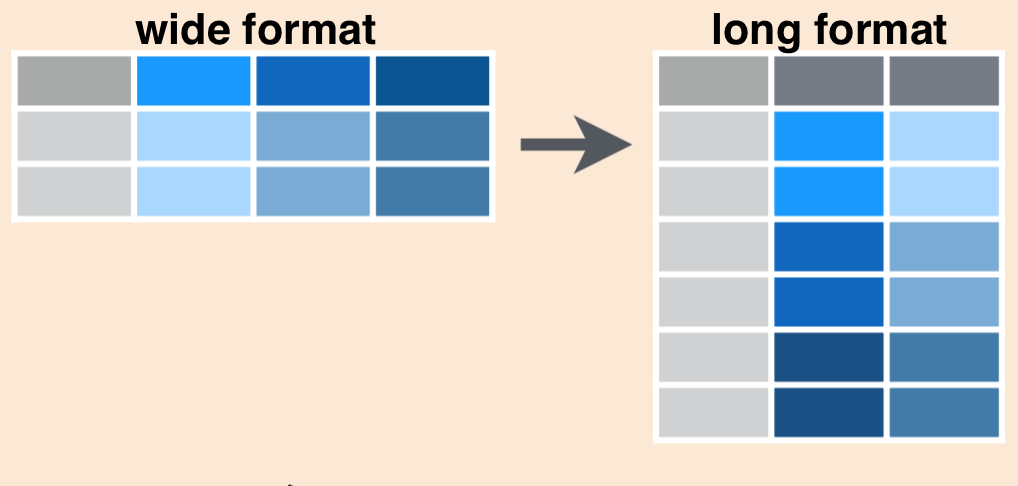
\includegraphics{img/tidyr_pivot_longer.png}

Generally, the code to gather wide columns together using \texttt{tidyr::pivot\_longer()} looks like this:

TODO: Add pivot\_longer() schematic

We'll use \texttt{tidyr::pivot\_longer()} to gather data from all years in \emph{inverts\_df} into two columns: one called \emph{year}, which contains the year (as a number), and another called \emph{sp\_count} that contains the number of each species observed. The new data frame will be stored as \emph{inverts\_long}:

\begin{Shaded}
\begin{Highlighting}[]
\NormalTok{inverts_long <-}\StringTok{ }\NormalTok{tidyr}\OperatorTok{::}\KeywordTok{pivot_longer}\NormalTok{(}\DataTypeTok{data =}\NormalTok{ inverts_df, }
                                    \DataTypeTok{cols =} \StringTok{'2016'}\OperatorTok{:}\StringTok{'2018'}\NormalTok{,}
                                    \DataTypeTok{names_to =} \StringTok{"year"}\NormalTok{,}
                                    \DataTypeTok{values_to =} \StringTok{"sp_count"}\NormalTok{)}
\end{Highlighting}
\end{Shaded}

The outcome is the new long-format \emph{inverts\_long} data frame:

\begin{Shaded}
\begin{Highlighting}[]
\NormalTok{inverts_long}
\end{Highlighting}
\end{Shaded}

\begin{verbatim}
## # A tibble: 165 x 5
##    month site  common_name              year  sp_count
##    <chr> <chr> <chr>                    <chr>    <dbl>
##  1 7     abur  california cone snail    2016       451
##  2 7     abur  california cone snail    2017        28
##  3 7     abur  california cone snail    2018       762
##  4 7     abur  california spiny lobster 2016        17
##  5 7     abur  california spiny lobster 2017        17
##  6 7     abur  california spiny lobster 2018        16
##  7 7     abur  orange cup coral         2016        24
##  8 7     abur  orange cup coral         2017        24
##  9 7     abur  orange cup coral         2018        24
## 10 7     abur  purple urchin            2016        48
## # ... with 155 more rows
\end{verbatim}

Hooray, long format!

One thing that isn't obvious at first (but would become obvious if you continued working with this data) is that since those year numbers were initially column names (characters), when they are stacked into the \emph{year} column, their class wasn't auto-updated to numeric.

Explore the class of \emph{year} in \emph{inverts\_long}:

\begin{Shaded}
\begin{Highlighting}[]
\KeywordTok{class}\NormalTok{(inverts_long}\OperatorTok{$}\NormalTok{year)}
\end{Highlighting}
\end{Shaded}

\begin{verbatim}
## [1] "character"
\end{verbatim}

We'll use \texttt{dplyr::mutate()} in a different way here: to create a new column (that's how we've used \texttt{mutate()} previously) that has the same name of an existing column, in order to update and overwrite the existing column.

In this case, we'll \texttt{mutate()} to add a column called \emph{year}, which contains an \texttt{as.numeric()} version of the existing \emph{year} variable:

\begin{Shaded}
\begin{Highlighting}[]
\CommentTok{# Coerce "year" class to numeric: }

\NormalTok{inverts_long <-}\StringTok{ }\NormalTok{inverts_long }\OperatorTok\StringTok{ }
\StringTok{  }\KeywordTok{mutate}\NormalTok{(}\DataTypeTok{year =} \KeywordTok{as.numeric}\NormalTok{(year))}
\end{Highlighting}
\end{Shaded}

Checking the class again, we see that \emph{year} has been updated to a numeric variable:

\begin{Shaded}
\begin{Highlighting}[]
\KeywordTok{class}\NormalTok{(inverts_long}\OperatorTok{$}\NormalTok{year)}
\end{Highlighting}
\end{Shaded}

\begin{verbatim}
## [1] "numeric"
\end{verbatim}

\hypertarget{long-to-wider-format-with-tidyrpivot_wider}{%
\subsubsection{\texorpdfstring{Long-to-wider format with \texttt{tidyr::pivot\_wider()}}{Long-to-wider format with tidyr::pivot\_wider()}}\label{long-to-wider-format-with-tidyrpivot_wider}}

In the previous example, we had information spread over multiple columns that we wanted to \emph{gather}. Sometimes, we'll have data that we want to \emph{spread} over multiple columns.

For example, imagine that starting from \emph{inverts\_long} we want each species in the \emph{common\_name} column to exist as its \textbf{own column}. In that case, we would be converting from a longer to a wider format, and will use \texttt{tidyr::pivot\_wider()} as follows:

TODO: Add pivot\_wider() schematic

Specifically for our data, we write code to spread the \emph{common\_name} column as follows:

\begin{Shaded}
\begin{Highlighting}[]
\NormalTok{inverts_wide <-}\StringTok{ }\NormalTok{inverts_long }\OperatorTok\StringTok{ }
\StringTok{  }\NormalTok{tidyr}\OperatorTok{::}\KeywordTok{pivot_wider}\NormalTok{(}\DataTypeTok{names_from =}\NormalTok{ common_name, }
                     \DataTypeTok{values_from =}\NormalTok{ sp_count)}
\end{Highlighting}
\end{Shaded}

\begin{Shaded}
\begin{Highlighting}[]
\NormalTok{inverts_wide}
\end{Highlighting}
\end{Shaded}

\begin{verbatim}
## # A tibble: 33 x 8
##    month site   year `california con~ `california spi~ `orange cup cor~
##    <chr> <chr> <dbl>            <dbl>            <dbl>            <dbl>
##  1 7     abur   2016              451               17               24
##  2 7     abur   2017               28               17               24
##  3 7     abur   2018              762               16               24
##  4 7     ahnd   2016               27               16               24
##  5 7     ahnd   2017               24               16               24
##  6 7     ahnd   2018               24               16               24
##  7 7     aque   2016             4971               48             1526
##  8 7     aque   2017             1752               48             1623
##  9 7     aque   2018             2616               48             1859
## 10 7     bull   2016             1735               24               36
## # ... with 23 more rows, and 2 more variables: `purple urchin` <dbl>,
## #   `rock scallop` <dbl>
\end{verbatim}

We can see that now each \emph{species} has its own column (wider format). But also notice that those column headers (since they have spaces) might not be in the most coder-friendly format\ldots{}

\hypertarget{meet-the-janitor-package}{%
\subsubsection{\texorpdfstring{Meet the \texttt{janitor} package}{Meet the janitor package}}\label{meet-the-janitor-package}}

The \texttt{janitor} package by Sam Firke is a brilliant collection of functions for some quick data cleaning. We recommend that you explore the different functions it contains. Like:

\begin{itemize}
\tightlist
\item
  \texttt{janitor::clean\_names()}: update column headers to a case of your choosing
\item
  \texttt{janitor::get\_dupes()}: see all rows that are duplicates within variables you choose
\item
  \texttt{janitor::remove\_empty()}: remove empty rows and/or columns
\item
  \texttt{janitor::andorn\_*()}: jazz up frequency tables of counts (we'll return to this for a table example in TODO: Session 8)
\item
  \ldots{}and more!
\end{itemize}

Here, we'll use \texttt{janitor::clean\_names()} to convert all of our column headers to a more convenient case - the default is \textbf{lower\_snake\_case}, which means all spaces and symbols are replaced with an underscore (or a word describing the symbol), all characters are lowercase, and a few other nice adjustments.

For example, \texttt{janitor::clean\_names()} would update these nightmare column names into much nicer forms:

\begin{itemize}
\tightlist
\item
  \texttt{My...RECENT-income!} becomes \texttt{my\_recent\_income}
\item
  \texttt{SAMPLE2.!test1} becomes \texttt{sample2\_test1}
\item
  \texttt{ThisIsTheName} becomes \texttt{this\_is\_the\_name}
\item
  \texttt{2015} becomes \texttt{x2015}
\end{itemize}

If we wanted to then use these columns (which we probably would, since we created them), we could clean the names to get them into more coder-friendly lower\_snake\_case with \texttt{janitor::clean\_names()}:

\begin{Shaded}
\begin{Highlighting}[]
\NormalTok{inverts_wide <-}\StringTok{ }\NormalTok{inverts_wide }\OperatorTok\StringTok{ }
\StringTok{  }\NormalTok{janitor}\OperatorTok{::}\KeywordTok{clean_names}\NormalTok{()}
\end{Highlighting}
\end{Shaded}

\begin{Shaded}
\begin{Highlighting}[]
\KeywordTok{names}\NormalTok{(inverts_wide)}
\end{Highlighting}
\end{Shaded}

\begin{verbatim}
## [1] "month"                    "site"                    
## [3] "year"                     "california_cone_snail"   
## [5] "california_spiny_lobster" "orange_cup_coral"        
## [7] "purple_urchin"            "rock_scallop"
\end{verbatim}

And there are other options for the case, like:

\begin{itemize}
\tightlist
\item
  ``snake'' produces snake\_case
\item
  ``lower\_camel'' or ``small\_camel'' produces lowerCamel
\item
  ``upper\_camel'' or ``big\_camel'' produces UpperCamel
\item
  ``screaming\_snake'' or ``all\_caps'' produces ALL\_CAPS
\item
  ``lower\_upper'' produces lowerUPPER
\item
  ``upper\_lower'' produces UPPERlower
\end{itemize}

\hypertarget{combine-or-separate-information-in-columns-with-tidyrunite-and-tidyrseparate}{%
\subsection{\texorpdfstring{Combine or separate information in columns with \texttt{tidyr::unite()} and \texttt{tidyr::separate()}}{Combine or separate information in columns with tidyr::unite() and tidyr::separate()}}\label{combine-or-separate-information-in-columns-with-tidyrunite-and-tidyrseparate}}

Sometimes we'll want to \emph{separate} contents of a single column into multiple columns, or \emph{combine} entries from different columns into a single column.

For example, the following data frame has \emph{genus} and \emph{species} in separate columns:

id

genus

species

common\_name

1

Scorpaena

guttata

sculpin

2

Sebastes

miniatus

vermillion

We may want to combine the genus and species into a single column, \emph{scientific\_name}:

id

scientific\_name

common\_name

1

Scorpaena guttata

sculpin

2

Sebastes miniatus

vermillion

Or we may want to do the reverse (separate information from a single column into multiple columns). Here, we'll learn \texttt{tidyr::unite()} and \texttt{tidyr::separate()} to help us do both.

\hypertarget{tidyrunite-to-merge-information-from-separate-columns}{%
\subsubsection{\texorpdfstring{\texttt{tidyr::unite()} to merge information from separate columns}{tidyr::unite() to merge information from separate columns}}\label{tidyrunite-to-merge-information-from-separate-columns}}

Use \texttt{tidyr::unite()} to combine (paste) information from multiple columns into a single column (as for the scientific name example above)

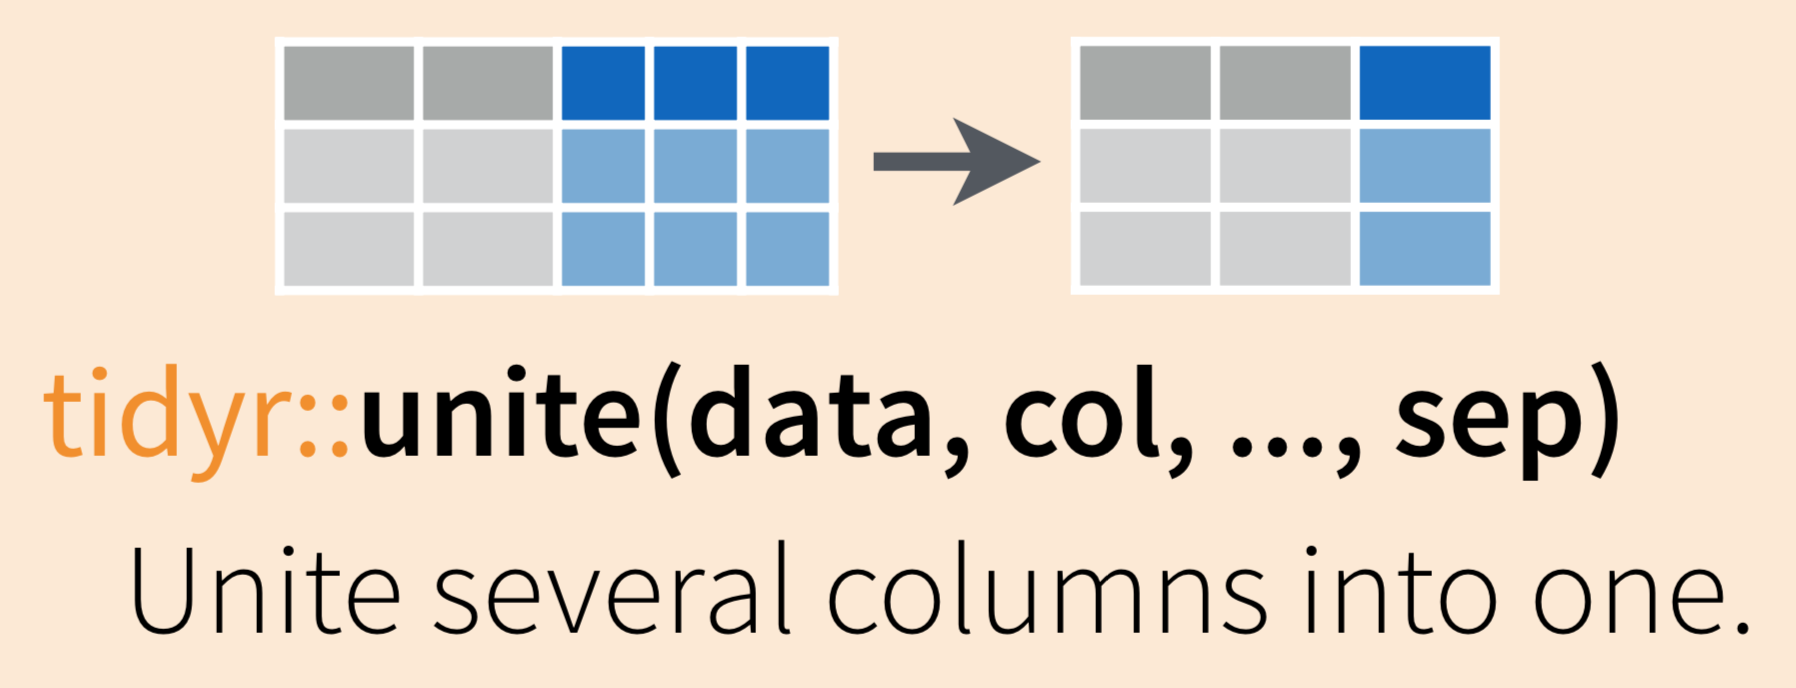
\includegraphics{img/rstudio-cheatsheet-unite.png}

To demonstrate uniting information from separate columns, we'll make a single column that has the combined information from \emph{site} abbreviation and \emph{year} in \emph{inverts\_wide}.

We need to give \texttt{tidyr::unite()} several arguments:

\begin{itemize}
\tightlist
\item
  \textbf{data:} the data frame containing columns we want to combine (or pipe into the function from the data frame)
\item
  \textbf{col:} the name of the new ``united'' column
\item
  the \textbf{columns you are uniting}
\item
  \textbf{sep:} the symbol, value or character to put between the united information from each column
\end{itemize}

\begin{Shaded}
\begin{Highlighting}[]
\NormalTok{inverts_unite <-}\StringTok{ }\NormalTok{inverts_wide }\OperatorTok\StringTok{ }
\StringTok{  }\NormalTok{tidyr}\OperatorTok{::}\KeywordTok{unite}\NormalTok{(}\DataTypeTok{col =} \StringTok{"site_year"}\NormalTok{, }\CommentTok{# What to name the new united column}
               \KeywordTok{c}\NormalTok{(site, year), }\CommentTok{# The columns we'll unite (site, year)}
               \DataTypeTok{sep =} \StringTok{"_"}\NormalTok{) }\CommentTok{# How to separate the things we're uniting}
\end{Highlighting}
\end{Shaded}

\begin{verbatim}
## # A tibble: 6 x 7
##   month site_year california_cone~ california_spin~ orange_cup_coral
##   <chr> <chr>                <dbl>            <dbl>            <dbl>
## 1 7     abur_2016              451               17               24
## 2 7     abur_2017               28               17               24
## 3 7     abur_2018              762               16               24
## 4 7     ahnd_2016               27               16               24
## 5 7     ahnd_2017               24               16               24
## 6 7     ahnd_2018               24               16               24
## # ... with 2 more variables: purple_urchin <dbl>, rock_scallop <dbl>
\end{verbatim}

Try updating the separator from "\_" to ``\emph{hello!}'' to see what the outcome column contains.

\texttt{tidyr::unite()} can also combine information from \emph{more} than two columns. For example, to combine the \emph{site}, \emph{common\_name} and \emph{year} columns from \emph{inverts\_long}, we could use:

\begin{Shaded}
\begin{Highlighting}[]
\CommentTok{# Uniting more than 2 columns: }

\NormalTok{inverts_triple_unite <-}\StringTok{ }\NormalTok{inverts_long }\OperatorTok\StringTok{ }
\StringTok{  }\NormalTok{tidyr}\OperatorTok{::}\KeywordTok{unite}\NormalTok{(}\DataTypeTok{col =} \StringTok{"year_site_name"}\NormalTok{,}
               \KeywordTok{c}\NormalTok{(year, site, common_name),}
               \DataTypeTok{sep =} \StringTok{"-"}\NormalTok{)}
\end{Highlighting}
\end{Shaded}

\begin{Shaded}
\begin{Highlighting}[]
\KeywordTok{head}\NormalTok{(inverts_triple_unite)}
\end{Highlighting}
\end{Shaded}

\begin{verbatim}
## # A tibble: 6 x 3
##   month year_site_name                     sp_count
##   <chr> <chr>                                 <dbl>
## 1 7     2016-abur-california cone snail         451
## 2 7     2017-abur-california cone snail          28
## 3 7     2018-abur-california cone snail         762
## 4 7     2016-abur-california spiny lobster       17
## 5 7     2017-abur-california spiny lobster       17
## 6 7     2018-abur-california spiny lobster       16
\end{verbatim}

\hypertarget{tidyrseparate-to-separate-information-into-multiple-columns}{%
\subsubsection{\texorpdfstring{\texttt{tidyr::separate()} to separate information into multiple columns}{tidyr::separate() to separate information into multiple columns}}\label{tidyrseparate-to-separate-information-into-multiple-columns}}

While \texttt{tidyr::unite()} allows us to combine information from multiple columns, it's more likely that you'll \emph{start} with a single column that you want to split up into pieces.

For example, I might want to split up a column containing the \emph{genus} and \emph{species} (\emph{Scorpaena guttata}) into two separate columns (\emph{Scorpaena} \textbar{} \emph{guttata}), so that I can count how many \emph{Scorpaena} organisms exist in my dataset at the genus level.

Use \texttt{tidyr::separate()} to ``separate a character column into multiple columns using a regular expression separator.''

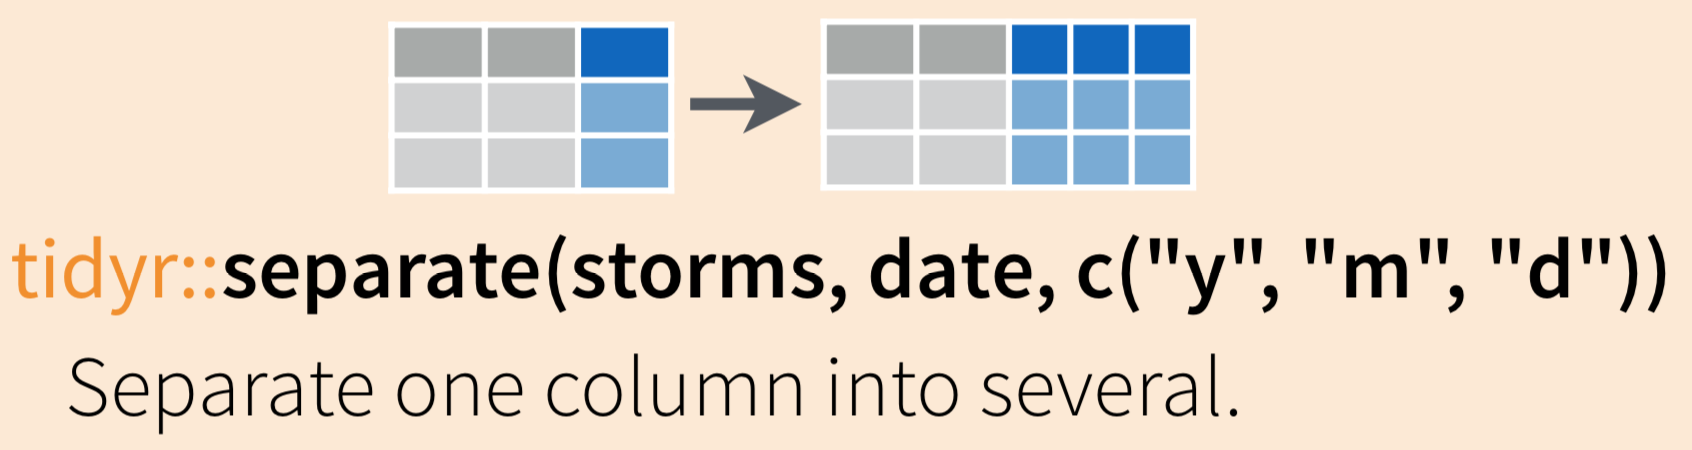
\includegraphics{img/rstudio-cheatsheet-separate.png}

Let's start again with \emph{inverts\_unite}, where we have combined the \emph{site} and \emph{year} into a single column called \emph{site\_year}. If we want to \textbf{separate} those, we can use:

\begin{Shaded}
\begin{Highlighting}[]
\NormalTok{inverts_sep <-}\StringTok{ }\NormalTok{inverts_triple_unite }\OperatorTok\StringTok{ }
\StringTok{  }\NormalTok{tidyr}\OperatorTok{::}\KeywordTok{separate}\NormalTok{(year_site_name, }\DataTypeTok{into =} \KeywordTok{c}\NormalTok{(}\StringTok{"my_year"}\NormalTok{, }\StringTok{"my_site_name"}\NormalTok{))}
\end{Highlighting}
\end{Shaded}

\begin{verbatim}
## Warning: Expected 2 pieces. Additional pieces discarded in 165 rows [1, 2,
## 3, 4, 5, 6, 7, 8, 9, 10, 11, 12, 13, 14, 15, 16, 17, 18, 19, 20, ...].
\end{verbatim}

What is that warning \texttt{Expected\ 2\ pieces...} telling us? If we take a look at the resulting data frame \emph{inverts\_sep}, we see that it only keeps the first \textbf{two} pieces, and gets rid of the third (name). Which is a bit concerning, because we rarely want to just throw away information in a data frame.

\begin{Shaded}
\begin{Highlighting}[]
\KeywordTok{head}\NormalTok{(inverts_sep)}
\end{Highlighting}
\end{Shaded}

\begin{verbatim}
## # A tibble: 6 x 4
##   month my_year my_site_name sp_count
##   <chr> <chr>   <chr>           <dbl>
## 1 7     2016    abur              451
## 2 7     2017    abur               28
## 3 7     2018    abur              762
## 4 7     2016    abur               17
## 5 7     2017    abur               17
## 6 7     2018    abur               16
\end{verbatim}

That's problematic. How can we make sure we're keeping as many different elements as exist in the united column?

We have a couple of options:

\begin{enumerate}
\def\labelenumi{\arabic{enumi}.}
\tightlist
\item
  Create the \emph{number} of columns that are needed to retain as many elements as exist (in this case, 3, but we only created two new columns in the example above)
\end{enumerate}

\begin{Shaded}
\begin{Highlighting}[]
\NormalTok{inverts_sep3 <-}\StringTok{ }\NormalTok{inverts_triple_unite }\OperatorTok\StringTok{ }
\StringTok{  }\NormalTok{tidyr}\OperatorTok{::}\KeywordTok{separate}\NormalTok{(year_site_name, }\DataTypeTok{into =} \KeywordTok{c}\NormalTok{(}\StringTok{"the_year"}\NormalTok{, }\StringTok{"the_site"}\NormalTok{, }\StringTok{"the_name"}\NormalTok{))}
\end{Highlighting}
\end{Shaded}

\begin{verbatim}
## Warning: Expected 3 pieces. Additional pieces discarded in 165 rows [1, 2,
## 3, 4, 5, 6, 7, 8, 9, 10, 11, 12, 13, 14, 15, 16, 17, 18, 19, 20, ...].
\end{verbatim}

Another warning. What is that about? Let's take a look at the resulting data frame and think about what's missing (what are the ``pieces discarded''?):

\begin{Shaded}
\begin{Highlighting}[]
\KeywordTok{head}\NormalTok{(inverts_sep3)}
\end{Highlighting}
\end{Shaded}

\begin{verbatim}
## # A tibble: 6 x 5
##   month the_year the_site the_name   sp_count
##   <chr> <chr>    <chr>    <chr>         <dbl>
## 1 7     2016     abur     california      451
## 2 7     2017     abur     california       28
## 3 7     2018     abur     california      762
## 4 7     2016     abur     california       17
## 5 7     2017     abur     california       17
## 6 7     2018     abur     california       16
\end{verbatim}

Aha! Only the \emph{first word} of the common name was retained, and anything else was trashed. We want to keep everything after the second dash in the new \emph{the\_name} column.

That's because the \textbf{default is \texttt{extra\ =\ "warn"}}, which means that if you have more pieces than columns you're separating into, it will populate the columns that have been allotted (in our case, just 3) then drop any additional information, giving you a warning that pieces have been dropped.

To keep the extra pieces that have been dropped, add the \texttt{extra\ =\ "merge"} argument within \texttt{tidyr::separate()} to override:

\begin{Shaded}
\begin{Highlighting}[]
\NormalTok{inverts_sep_all <-}\StringTok{ }\NormalTok{inverts_triple_unite }\OperatorTok\StringTok{ }
\StringTok{  }\KeywordTok{separate}\NormalTok{(year_site_name, }
           \DataTypeTok{into =} \KeywordTok{c}\NormalTok{(}\StringTok{"sample_year"}\NormalTok{, }\StringTok{"location"}\NormalTok{, }\StringTok{"sp_name"}\NormalTok{), }
           \DataTypeTok{extra =} \StringTok{"merge"}\NormalTok{)}
\end{Highlighting}
\end{Shaded}

No warning there about things being discarded. Explore \emph{inverts\_sep\_all}:

\begin{verbatim}
## # A tibble: 165 x 5
##    month sample_year location sp_name                  sp_count
##    <chr> <chr>       <chr>    <chr>                       <dbl>
##  1 7     2016        abur     california cone snail         451
##  2 7     2017        abur     california cone snail          28
##  3 7     2018        abur     california cone snail         762
##  4 7     2016        abur     california spiny lobster       17
##  5 7     2017        abur     california spiny lobster       17
##  6 7     2018        abur     california spiny lobster       16
##  7 7     2016        abur     orange cup coral               24
##  8 7     2017        abur     orange cup coral               24
##  9 7     2018        abur     orange cup coral               24
## 10 7     2016        abur     purple urchin                  48
## # ... with 155 more rows
\end{verbatim}

We see that the resulting data frame has split \emph{year\_site\_name} into three separate columns, \emph{sample\_year}, \emph{location}, and \emph{sp\_name}, but now everything after the second break (``-'') remains together in \emph{sp\_name} instead of dropping pieces following the third word.

\hypertarget{convert-between-explicit-and-implicit-missings-nas}{%
\subsection{\texorpdfstring{Convert between explicit and implicit missings (\texttt{NA}s)}{Convert between explicit and implicit missings (NAs)}}\label{convert-between-explicit-and-implicit-missings-nas}}

An \emph{explicit missing} is when every possible outcome actually appears in a data frame as a row, even if a variable of interest for that row is missing (\texttt{NA}).

Conversely, an \emph{implicit missing} is when an observation (row) does \emph{not} appear in the data frame because a variable of interest contains an \texttt{NA} missing value.

Consider the following data:

day

animal

food\_choice

Monday

eagle

fish

Monday

mountain lion

squirrel

Monday

toad

NA

Tuesday

eagle

fish

Tuesday

mountain lion

deer

Tuesday

toad

flies

Notice that the row for \textbf{toad} still appears in the dataset for \textbf{Tuesday}, despite having a missing food choice for that day. This is an \emph{explicit missing} because the row still appears in the data frame.

If that row was removed, the resulting dataset would look like this:

\begin{Shaded}
\begin{Highlighting}[]
\NormalTok{df_missings }\OperatorTok\StringTok{ }
\StringTok{  }\KeywordTok{drop_na}\NormalTok{(food_choice) }\OperatorTok\StringTok{ }
\StringTok{  }\KeywordTok{kable}\NormalTok{()}
\end{Highlighting}
\end{Shaded}

day

animal

food\_choice

Monday

eagle

fish

Monday

mountain lion

squirrel

Tuesday

eagle

fish

Tuesday

mountain lion

deer

Tuesday

toad

flies

\ldots{}and if your reaction is ``But then how do I know there's a toad from \textbf{MONDAY}?'', then you can see how it can be a bit risky to have \emph{implicit missings} instead of \emph{explicit missings}.

Whichever we choose, we can convert between the two forms using \texttt{tidyr::drop\_na()} or \texttt{tidyr::complete()}:

\begin{itemize}
\tightlist
\item
  \texttt{tidyr::drop\_na()}: removes observations (rows) that contain \texttt{NA} for variable(s) of interest
\item
  \texttt{tidyr::complete()}: turns implicit missing values into explicit missing values by completing a data frame with missing combinations of data
\end{itemize}

We'll use both here, starting with the \emph{inverts\_long} data frame we created above.

Looking through \emph{inverts\_long}, we'll see that there are \texttt{NA} observations for every species at site \textbf{bull} in 2018 - but those \texttt{NA} counts do show up. First, we'll use \texttt{tidyr::drop\_na()} to make those missings implicit (invisible) instead:

\begin{Shaded}
\begin{Highlighting}[]
\NormalTok{inverts_implicit_NA <-}\StringTok{ }\NormalTok{inverts_long }\OperatorTok\StringTok{ }
\StringTok{  }\KeywordTok{drop_na}\NormalTok{(sp_count)}
\end{Highlighting}
\end{Shaded}

See that now, the rows that contained an \texttt{NA} in the \emph{sp\_count} column from \emph{inverts\_long} have been removed.

WAIT, I want them back! We can ask R to create explicit missings (by identifying which combinations of groups currently don't appear in the data frame) using \texttt{tidyr::complete()}:

\begin{Shaded}
\begin{Highlighting}[]
\NormalTok{inverts_explicit_NA <-}\StringTok{ }\NormalTok{inverts_implicit_NA }\OperatorTok\StringTok{ }
\StringTok{  }\KeywordTok{complete}\NormalTok{(month, site, common_name, year)}
\end{Highlighting}
\end{Shaded}

Now you'll see \texttt{inverts\_explicit\_NA} has those 5 ``missing'' observations shown in the data frame.

\hypertarget{activities}{%
\subsection{Activities}\label{activities}}

TODO

\hypertarget{fun-facts-insights}{%
\subsection{Fun facts / insights}\label{fun-facts-insights}}

TODO

\hypertarget{vlookup}{%
\chapter{Dplyr and vlookups}\label{vlookup}}

\hypertarget{summary-5}{%
\section{Summary}\label{summary-5}}

In previous sessions, we've learned to do some basic wrangling and find summary information with functions in the \texttt{dplyr} package, which exists within the \texttt{tidyverse}. We've used:

TODO: Check these to make sure what we do in 1 - 4!

\begin{itemize}
\tightlist
\item
  \texttt{dplyr::count()} and \texttt{dplyr::uncount()} to get counts of observations for groupings we specify (or the reverse!)
\item
  \texttt{dplyr::mutate()}: \textbf{add} a new column, while keeping the existing ones
\item
  \texttt{dplyr::group\_by()}: let R know that \textbf{groups} exist within the dataset, by variable(s)
\item
  \texttt{dplyr::summarize()}: calculate a value (that you specify) for each group, then report each group's value in a table
\end{itemize}

In Session 5, we'll expand our data wrangling toolkit using:

\begin{itemize}
\tightlist
\item
  \texttt{dplyr::filter()} to conditionally subset our data by \textbf{rows}, and
\item
  \texttt{dplyr::*\_join()} functions to merge data frames together
\end{itemize}

The combination of \texttt{dplyr::filter()} and \texttt{dplyr::*\_join()} - to return rows satisfying a condition we specify, and merging data frames by like variables - is analogous to the useful VLOOKUP function in Excel.

\hypertarget{objectives-4}{%
\section{Objectives}\label{objectives-4}}

\begin{itemize}
\tightlist
\item
  Continue building R Markdown skills
\item
  Return \textbf{rows} that satisfy variable conditions using \texttt{dplyr::filter()}
\item
  Use \texttt{dplyr::full\_join()}, \texttt{dplyr::left\_join()}, and \texttt{dplyr::inner\_join()} to merge data frames by matching variables, with different endpoints in mind
\item
  Use \texttt{dplyr::anti\_join()} to find things that \textbf{do not} exist in both data frames
\item
  Understand the similarities between \texttt{dplyr::filter()} + \texttt{dplyr::*\_join()} and Excel's VLOOKUP function
\end{itemize}

\hypertarget{resources-7}{%
\section{Resources}\label{resources-7}}

\begin{itemize}
\tightlist
\item
  \href{https://dplyr.tidyverse.org/reference/filter.html}{\texttt{dplyr::filter()} documentation from tidyverse.org}
\item
  \href{https://dplyr.tidyverse.org/reference/join.html}{\texttt{dplyr::join()} documentation from tidyverse.org}
\item
  \href{https://r4ds.had.co.nz/}{Chapters 5 and 13 in \emph{R for Data Science} by Garrett Grolemund and Hadley Wickham}
\end{itemize}

\hypertarget{lessons}{%
\section{Lessons}\label{lessons}}

\textbf{Session 5 set-up:} TODO

\begin{itemize}
\tightlist
\item
  Create a new .Rmd within the r-and-excel directory (project) you created in Session 1
\item
  Add some descriptive text
\item
  Add new code chunks to:

  \begin{itemize}
  \tightlist
  \item
    Attach packages
  \item
    Read in the necessary data
  \end{itemize}
\end{itemize}

In this session we'll use the \textbf{fish\_counts\_curated.csv} and \textbf{invert\_counts\_curated.xlsx} files, and the first worksheet from \textbf{kelp\_counts\_curated.xlsx}.

\begin{Shaded}
\begin{Highlighting}[]
\CommentTok{# Attach packages:}
\KeywordTok{library}\NormalTok{(tidyverse)}
\KeywordTok{library}\NormalTok{(readxl)}

\CommentTok{# Read in data: }
\NormalTok{invert_counts <-}\StringTok{ }\KeywordTok{read_excel}\NormalTok{(}\StringTok{"invert_counts_curated.xlsx"}\NormalTok{)}
\NormalTok{fish_counts <-}\StringTok{ }\KeywordTok{read_csv}\NormalTok{(}\StringTok{"fish_counts_curated.csv"}\NormalTok{)}
\NormalTok{kelp_counts_abur <-}\StringTok{ }\KeywordTok{read_excel}\NormalTok{(}\StringTok{"kelp_counts_curated.xlsx"}\NormalTok{)}
\end{Highlighting}
\end{Shaded}

Remember to always explore the data you've read in using functions like \texttt{View()}, \texttt{names()}, \texttt{summary()}, \texttt{head()} and \texttt{tail()} to ensure that the data you \emph{think} you read in is \emph{actually} the data you read in.

Now, let's use \texttt{dplyr::filter()} to decide which observations (rows) we'll keep or exclude in new subsets, similar to using Excel's VLOOKUP function.

\hypertarget{dplyrfilter-to-conditionally-subset-by-rows}{%
\subsection{\texorpdfstring{\texttt{dplyr::filter()} to conditionally subset by rows}{dplyr::filter() to conditionally subset by rows}}\label{dplyrfilter-to-conditionally-subset-by-rows}}

Use \texttt{dplyr::filter()} to let R know which \textbf{rows} you want to keep or exclude, based whether or not their contents match conditions that you set for one or more variables.

\begin{figure}
\centering
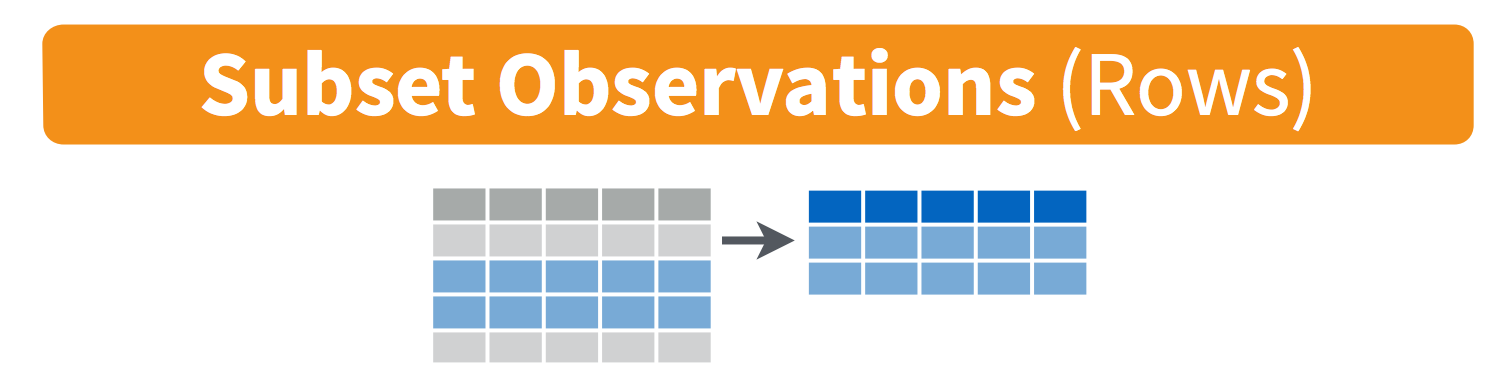
\includegraphics{img/rstudio-cheatsheet-filter.png}
\caption{dplyr::filter()}
\end{figure}

Some examples in words that might inspire you to use \texttt{dplyr::filter()}:

\begin{itemize}
\tightlist
\item
  ``I only want to keep rows where the temperature is greater than 90°F.''
\item
  ``I want to keep all observations \textbf{except} those where the tree type is listed as \textbf{unknown}.''
\item
  ``I want to make a new subset with only data for mountain lions (the species variable) in California (the state variable).''
\end{itemize}

When we use \texttt{dplyr::filter()}, we need to let R know a couple of things:

\begin{itemize}
\tightlist
\item
  What data frame we're filtering from
\item
  What condition(s) we want observations to \textbf{match} and/or \textbf{not match} in order to keep them in the new subset
\end{itemize}

Follow along with the examples below to learn some common ways to use \texttt{dplyr::filter()}.

\hypertarget{filter-rows-by-matching-a-single-character-string}{%
\subsubsection{Filter rows by matching a single character string}\label{filter-rows-by-matching-a-single-character-string}}

Let's say we want to keep all observations from the fish\_counts data frame where the common name is ``garibaldi.'' Here, we need to tell R to only \emph{keep rows} from the \textbf{fish\_counts} data frame when the common name (\textbf{common\_name} variable) exactly matches \textbf{garibaldi}.
Use \texttt{==} to ask R to look for matching strings:

\begin{Shaded}
\begin{Highlighting}[]
\NormalTok{fish_gari <-}\StringTok{ }\NormalTok{dplyr}\OperatorTok{::}\KeywordTok{filter}\NormalTok{(fish_counts, common_name }\OperatorTok{==}\StringTok{ "garibaldi"}\NormalTok{)}
\end{Highlighting}
\end{Shaded}

Check out the \textbf{fish\_gari} object to ensure that only \emph{garibaldi} observations remain.

You could also do this using the pipe operator \texttt{\%\textgreater{}\%} (though for a single function, it doesn't save much effort or typing):

\begin{Shaded}
\begin{Highlighting}[]
\NormalTok{fish_gari <-}\StringTok{ }\NormalTok{fish_counts }\OperatorTok\StringTok{ }
\StringTok{  }\NormalTok{dplyr}\OperatorTok{::}\KeywordTok{filter}\NormalTok{(common_name }\OperatorTok{==}\StringTok{ "garibaldi"}\NormalTok{)}
\end{Highlighting}
\end{Shaded}

\hypertarget{filter-rows-based-on-numeric-conditions}{%
\subsubsection{Filter rows based on numeric conditions}\label{filter-rows-based-on-numeric-conditions}}

Use expected operators (\textgreater{}, \textless{}, \textgreater{}=, \textless{}=, =) to set conditions for a numeric variable when filtering. For this example, we only want to retain observations when the \textbf{total\_count} column value is \textgreater{}= 50:

\begin{Shaded}
\begin{Highlighting}[]
\NormalTok{fish_over50 <-}\StringTok{ }\NormalTok{dplyr}\OperatorTok{::}\KeywordTok{filter}\NormalTok{(fish_counts, total_count }\OperatorTok{>=}\StringTok{ }\DecValTok{50}\NormalTok{)}
\end{Highlighting}
\end{Shaded}

Or, using the pipe:

\begin{Shaded}
\begin{Highlighting}[]
\NormalTok{fish_over50 <-}\StringTok{ }\NormalTok{fish_counts }\OperatorTok\StringTok{ }
\StringTok{  }\NormalTok{dplyr}\OperatorTok{::}\KeywordTok{filter}\NormalTok{(total_count }\OperatorTok{>=}\StringTok{ }\DecValTok{50}\NormalTok{)}
\end{Highlighting}
\end{Shaded}

TODO: show example of between and exact =

\hypertarget{filter-to-return-rows-that-match-this-or-that-or-that}{%
\subsubsection{\texorpdfstring{Filter to return rows that match \emph{this} OR \emph{that} OR \emph{that}}{Filter to return rows that match this OR that OR that}}\label{filter-to-return-rows-that-match-this-or-that-or-that}}

What if we want to return a subset of the fish\_counts df that contains \emph{garibaldi}, \emph{blacksmith} OR \emph{black surfperch}?

There are several ways to write an ``OR'' statement for filtering, which will keep any observations that match Condition A \emph{or} Condition B \emph{or} Condition C. In this example, we will create a subset from \textbf{fish\_counts} that only contains rows where the \textbf{common\_name} is \emph{garibaldi} or \emph{blacksmith} or \emph{black surfperch}.

Use \texttt{\%in\%} to ask R to look for \emph{any matches} within a combined vector of strings:

\begin{Shaded}
\begin{Highlighting}[]
\NormalTok{fish_3sp <-}\StringTok{ }\NormalTok{fish_counts }\OperatorTok\StringTok{ }
\StringTok{  }\NormalTok{dplyr}\OperatorTok{::}\KeywordTok{filter}\NormalTok{(common_name }\OperatorTok\StringTok{ }\KeywordTok{c}\NormalTok{(}\StringTok{"garibaldi"}\NormalTok{, }\StringTok{"blacksmith"}\NormalTok{, }\StringTok{"black surfperch"}\NormalTok{))}
\end{Highlighting}
\end{Shaded}

Alternatively, you can indicate \textbf{OR} using the vertical line operator \texttt{\textbar{}} to do the same thing (but you can see that it's more repetitive when looking for matches within the same variable):

\begin{Shaded}
\begin{Highlighting}[]
\NormalTok{fish_3sp <-}\StringTok{ }\NormalTok{fish_counts }\OperatorTok\StringTok{ }
\StringTok{  }\NormalTok{dplyr}\OperatorTok{::}\KeywordTok{filter}\NormalTok{(common_name }\OperatorTok{==}\StringTok{ "garibaldi"} \OperatorTok{|}\StringTok{ }\NormalTok{common_name }\OperatorTok{==}\StringTok{ "blacksmith"} \OperatorTok{|}\StringTok{ }\NormalTok{common_name }\OperatorTok{==}\StringTok{ "black surfperch"}\NormalTok{)}
\end{Highlighting}
\end{Shaded}

\hypertarget{filter-to-return-rows-that-match-conditions-for-multiple-variables}{%
\subsubsection{Filter to return rows that match conditions for multiple variables}\label{filter-to-return-rows-that-match-conditions-for-multiple-variables}}

In the previous examples, we set filter conditions based on a single variable (e.g.~common\_name). What if we want to return observations that satisfy conditions for multiple variables?

For example: We want to create a subset that only returns rows from `invert\_counts' where the \textbf{site} is ``abur'' or ``mohk'' \emph{and} the \textbf{common\_name} is ``purple urchin.'' In \texttt{dplyr::filter()}, add a comma (or ampersand, \&) between arguments for multiple \emph{AND} conditions:

\begin{Shaded}
\begin{Highlighting}[]
\NormalTok{urchin_abur_mohk <-}\StringTok{ }\NormalTok{invert_counts }\OperatorTok\StringTok{ }
\StringTok{  }\NormalTok{dplyr}\OperatorTok{::}\KeywordTok{filter}\NormalTok{(site }\OperatorTok\StringTok{ }\KeywordTok{c}\NormalTok{(}\StringTok{"abur"}\NormalTok{,}\StringTok{"mohk"}\NormalTok{), common_name }\OperatorTok{==}\StringTok{ "purple urchin"}\NormalTok{)}
\end{Highlighting}
\end{Shaded}

\begin{Shaded}
\begin{Highlighting}[]
\KeywordTok{head}\NormalTok{(urchin_abur_mohk)}
\end{Highlighting}
\end{Shaded}

\begin{verbatim}
## # A tibble: 2 x 6
##   month site  common_name   `2016` `2017` `2018`
##   <chr> <chr> <chr>          <dbl>  <dbl>  <dbl>
## 1 7     abur  purple urchin     48     48     48
## 2 7     mohk  purple urchin    620    505    323
\end{verbatim}

Like most things in R, there are other ways to do the same thing. For example, you could do the same thing using \texttt{\&} (instead of a comma) between ``and'' conditions:

\begin{Shaded}
\begin{Highlighting}[]
\CommentTok{# Use the ampersand (&) to add another condition "and this must be true":}

\NormalTok{urchin_abur_mohk <-}\StringTok{ }\NormalTok{invert_counts }\OperatorTok\StringTok{ }
\StringTok{  }\NormalTok{dplyr}\OperatorTok{::}\KeywordTok{filter}\NormalTok{(site }\OperatorTok\StringTok{ }\KeywordTok{c}\NormalTok{(}\StringTok{"abur"}\NormalTok{,}\StringTok{"mohk"}\NormalTok{) }\OperatorTok{&}\StringTok{ }\NormalTok{common_name }\OperatorTok{==}\StringTok{ "purple urchin"}\NormalTok{)}
\end{Highlighting}
\end{Shaded}

Or you could just do two filter steps in sequence:

\begin{Shaded}
\begin{Highlighting}[]
\CommentTok{# Written as multiple filter steps:}

\NormalTok{urchin_abur_mohk <-}\StringTok{ }\NormalTok{invert_counts }\OperatorTok\StringTok{ }
\StringTok{  }\NormalTok{dplyr}\OperatorTok{::}\KeywordTok{filter}\NormalTok{(site }\OperatorTok\StringTok{ }\KeywordTok{c}\NormalTok{(}\StringTok{"abur"}\NormalTok{, }\StringTok{"mohk"}\NormalTok{)) }\OperatorTok\StringTok{ }
\StringTok{  }\NormalTok{dplyr}\OperatorTok{::}\KeywordTok{filter}\NormalTok{(common_name }\OperatorTok{==}\StringTok{ "purple urchin"}\NormalTok{)}
\end{Highlighting}
\end{Shaded}

\hypertarget{filter-to-return-rows-that-do-not-match-conditions}{%
\subsubsection{\texorpdfstring{Filter to return rows that \emph{do not} match conditions}{Filter to return rows that do not match conditions}}\label{filter-to-return-rows-that-do-not-match-conditions}}

Sometimes we might want to exclude observations. Here, let's say we want to make a subset that contains all rows from \textbf{fish\_counts} except those recorded at the Mohawk Reef site (``mohk'' in the \emph{site} variable).

We use \texttt{!=} to return observations that \textbf{do not match} a condition.

Like this:

\begin{Shaded}
\begin{Highlighting}[]
\NormalTok{fish_no_mohk <-}\StringTok{ }\NormalTok{fish_counts }\OperatorTok\StringTok{ }
\StringTok{  }\NormalTok{dplyr}\OperatorTok{::}\KeywordTok{filter}\NormalTok{(site }\OperatorTok{!=}\StringTok{ "mohk"}\NormalTok{)}
\end{Highlighting}
\end{Shaded}

This similarly works to exclude observations by a value.

For example, if we want to return all observations \emph{except} those where the total fish count is 1, we use:

\begin{Shaded}
\begin{Highlighting}[]
\NormalTok{fish_more_one <-}\StringTok{ }\NormalTok{fish_counts }\OperatorTok\StringTok{ }
\StringTok{  }\NormalTok{dplyr}\OperatorTok{::}\KeywordTok{filter}\NormalTok{(total_count }\OperatorTok{!=}\StringTok{ }\DecValTok{1}\NormalTok{)}
\end{Highlighting}
\end{Shaded}

What if we want to exclude observations for multiple conditions? For example, here we want to return all rows where the fish species \textbf{is not} garibaldi \textbf{or} rock wrasse.

We can use \texttt{filter(!variable\ \%in\%\ c("apple",\ "orange"))} to return rows where the variable does \textbf{not} match ``apple'' or ``orange''. For our fish example, that looks like this:

\begin{Shaded}
\begin{Highlighting}[]
\NormalTok{fish_subset <-}\StringTok{ }\NormalTok{fish_counts }\OperatorTok\StringTok{ }
\StringTok{  }\NormalTok{dplyr}\OperatorTok{::}\KeywordTok{filter}\NormalTok{(}\OperatorTok{!}\NormalTok{common_name }\OperatorTok\StringTok{ }\KeywordTok{c}\NormalTok{(}\StringTok{"garibaldi"}\NormalTok{, }\StringTok{"rock wrasse"}\NormalTok{))}
\end{Highlighting}
\end{Shaded}

Which then only returns observations for the other fish species in the dataset.

\begin{Shaded}
\begin{Highlighting}[]
\KeywordTok{head}\NormalTok{(fish_subset)}
\end{Highlighting}
\end{Shaded}

\begin{verbatim}
## # A tibble: 6 x 4
##    year site  common_name     total_count
##   <dbl> <chr> <chr>                 <dbl>
## 1  2016 abur  black surfperch           2
## 2  2016 abur  blacksmith                1
## 3  2016 abur  senorita                 58
## 4  2016 aque  black surfperch           1
## 5  2016 aque  blacksmith                1
## 6  2016 aque  senorita                 57
\end{verbatim}

\hypertarget{example-combining-filter-with-other-functions-using-the-pipe-operator}{%
\subsubsection{\texorpdfstring{Example: combining \texttt{filter()} with other functions using the pipe operator (\texttt{\%\textgreater{}\%})}{Example: combining filter() with other functions using the pipe operator (\%\textgreater{}\%)}}\label{example-combining-filter-with-other-functions-using-the-pipe-operator}}

We can also use \texttt{dplyr::filter()} in combination with the functions we previously learned for wrangling. If we have multiple sequential steps to perform, we can string them together using the \emph{pipe operator} (\texttt{\%\textgreater{}\%}).

Here, we'll start with the \texttt{invert\_counts} data frame and create a subset that:

TODO: NOPE, can't do this, they don't learn \texttt{pivot\_longer()} until the next section (tidying)

\begin{itemize}
\tightlist
\item
  Converts to long format with \texttt{pivot\_longer()}
\item
  Only keeps observations for rock scallops
\item
  Calculates the total count of rock scallops by site only
\end{itemize}

\begin{Shaded}
\begin{Highlighting}[]
\CommentTok{# Counts of scallops by site (all years included):}

\NormalTok{scallop_count_by_site <-}\StringTok{ }\NormalTok{invert_counts }\OperatorTok\StringTok{ }
\StringTok{  }\KeywordTok{pivot_longer}\NormalTok{(}\DataTypeTok{cols =} \StringTok{'2016'}\OperatorTok{:}\StringTok{'2018'}\NormalTok{, }
               \DataTypeTok{names_to =} \StringTok{"year"}\NormalTok{, }
               \DataTypeTok{values_to =} \StringTok{"sp_count"}\NormalTok{) }\OperatorTok\StringTok{ }
\StringTok{  }\KeywordTok{filter}\NormalTok{(common_name }\OperatorTok{==}\StringTok{ "rock scallop"}\NormalTok{) }\OperatorTok\StringTok{ }
\StringTok{  }\KeywordTok{group_by}\NormalTok{(site) }\OperatorTok\StringTok{ }
\StringTok{  }\KeywordTok{summarize}\NormalTok{(}\DataTypeTok{tot_count =} \KeywordTok{sum}\NormalTok{(sp_count, }\DataTypeTok{na.rm =} \OtherTok{TRUE}\NormalTok{))}
\end{Highlighting}
\end{Shaded}

\begin{Shaded}
\begin{Highlighting}[]
\NormalTok{scallop_count_by_site}
\end{Highlighting}
\end{Shaded}

\begin{verbatim}
## # A tibble: 11 x 2
##    site  tot_count
##    <chr>     <dbl>
##  1 abur         48
##  2 ahnd         48
##  3 aque        152
##  4 bull         48
##  5 carp       2519
##  6 golb         48
##  7 ivee        169
##  8 mohk        346
##  9 napl       6416
## 10 scdi       2390
## 11 sctw       1259
\end{verbatim}

\hypertarget{activity-1-using-filter-in-a-wrangling-sequence}{%
\subsubsection{\texorpdfstring{Activity 1: using \texttt{filter()} in a wrangling sequence}{Activity 1: using filter() in a wrangling sequence}}\label{activity-1-using-filter-in-a-wrangling-sequence}}

Write a sequence of code (connected by the pipe operator, \texttt{\%\textgreater{}\%}), to complete the following and store the output as object \texttt{my\_fish\_wrangling}:

\begin{itemize}
\tightlist
\item
  Starting from the \texttt{fish\_counts} data frame (stored earlier)
\item
  Only keep observations from \emph{Arroyo Burro} (site `abur')
\item
  Group by \emph{common\_name} (species)
\item
  Find total fish counts (by species) across all years
\end{itemize}

\hypertarget{merging-data-frames-with-dplyr_join}{%
\subsection{\texorpdfstring{Merging data frames with \texttt{dplyr::*\_join()}}{Merging data frames with dplyr::*\_join()}}\label{merging-data-frames-with-dplyr_join}}

Excel's \texttt{VLOOKUP} can also be used to merge data from separate tables or worksheets. Here, we'll use the \texttt{dplyr::*\_join()} functions to merge separate data frames in R.

There are a number of ways to merge data frames in R. We'll use \texttt{full\_join()}, \texttt{left\_join()}, and \texttt{inner\_join()} in this session.

From R Documentation (\texttt{?join}):

\begin{itemize}
\item
  \texttt{dplyr::full\_join()}: ``returns all rows and all columns from both x and y. Where there are not matching values, returns NA for the one missing.'' Basically, nothing gets thrown out, even if a match doesn't exist - making \texttt{full\_join()} the safest option for merging data frames. When in doubt, \texttt{full\_join()}.
\item
  \texttt{dplyr::left\_join()}: ``return all rows from x, and all columns from x and y. Rows in x with no match in y will have NA values in the new columns. If there are multiple matches between x and y, all combinations of the matches are returned.''
\item
  \texttt{dplyr::inner\_join()}: ``returns all rows from x where there are matching values in y, and all columns from x and y. If there are multiple matches between x and y, all combination of the matches are returned.'' This will drop observations that don't have a match between the merged data frames, which makes it a riskier merging option if you're not sure what you're trying to do.
\end{itemize}

Schematic (from RStudio data wrangling cheat sheet):
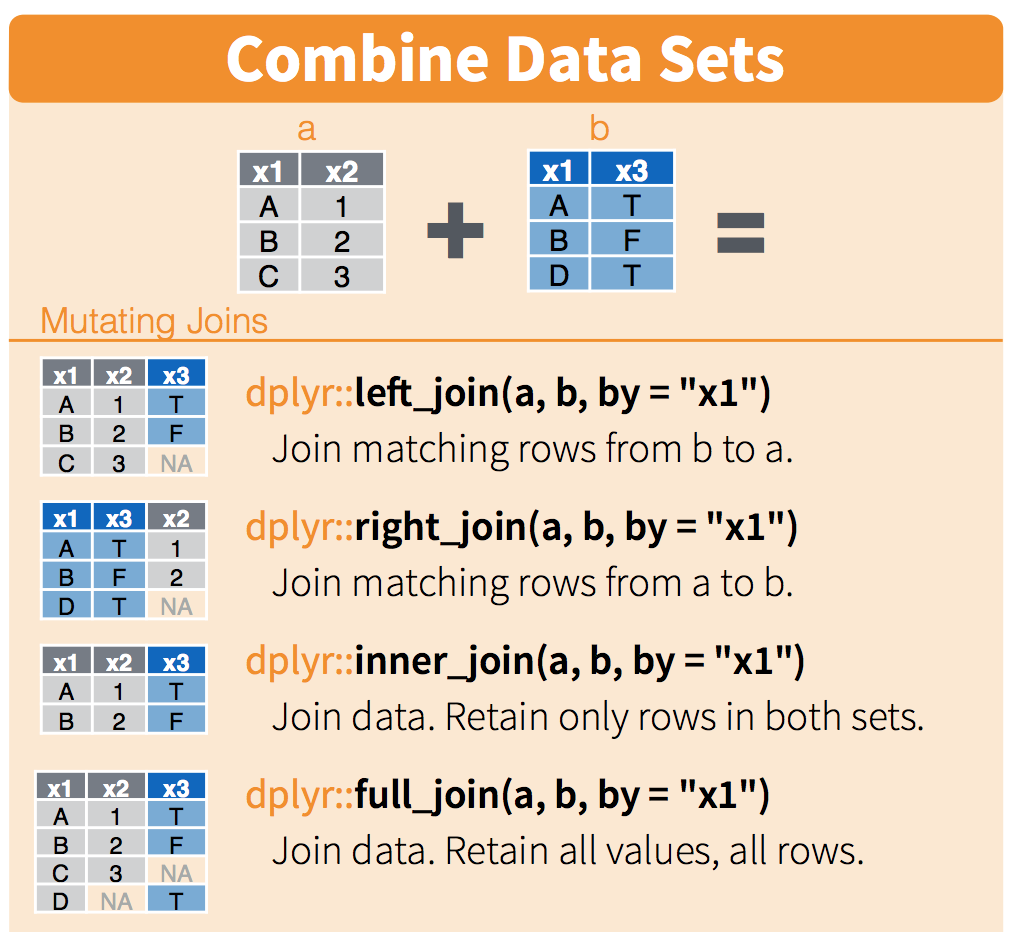
\includegraphics{img/rstudio-cheatsheet-combine-options1.png}

To clarify what the different joins are doing, let's first make a subset of the \emph{fish\_counts} data frame that only contains observations from 2016 and 2017.

\begin{Shaded}
\begin{Highlighting}[]
\NormalTok{fish_}\DecValTok{2016}\NormalTok{_}\DecValTok{2017}\NormalTok{ <-}\StringTok{ }\NormalTok{fish_counts }\OperatorTok\StringTok{ }
\StringTok{  }\KeywordTok{filter}\NormalTok{(year }\OperatorTok{==}\StringTok{ }\DecValTok{2016} \OperatorTok{|}\StringTok{ }\NormalTok{year }\OperatorTok{==}\StringTok{ }\DecValTok{2017}\NormalTok{)}
\end{Highlighting}
\end{Shaded}

Take a look to ensure that only those years are included with \texttt{View(fish\_2016\_2017)}. Now, let's merge it with our kelp fronds data in different ways.

\hypertarget{dplyrfull_join-to-merge-data-frames-keeping-everything}{%
\subsubsection{\texorpdfstring{\texttt{dplyr::full\_join()} to merge data frames, keeping everything}{dplyr::full\_join() to merge data frames, keeping everything}}\label{dplyrfull_join-to-merge-data-frames-keeping-everything}}

When we join data frames in R, we need to tell R a couple of things (and it does the hard joining work for us):

\begin{itemize}
\tightlist
\item
  Which data frames we want to merge together
\item
  Which variables to merge by
\end{itemize}

\textbf{Note:} If there are \textbf{exactly matching} column names in the data frames you're merging, the \texttt{*\_join()} functions will assume that you want to join by those columns. If there are \emph{no} matching column names, you can specify which columns to join by manually. We'll do both here.

\begin{Shaded}
\begin{Highlighting}[]
\CommentTok{# Join the fish_counts and kelp_counts_abur together: }
\NormalTok{abur_kelp_join <-}\StringTok{ }\NormalTok{fish_}\DecValTok{2016}\NormalTok{_}\DecValTok{2017} \OperatorTok\StringTok{ }
\StringTok{  }\KeywordTok{full_join}\NormalTok{(kelp_counts_abur) }\CommentTok{# Uh oh. An error message.}
\end{Highlighting}
\end{Shaded}

When we try to do that join, we get an error message:
\texttt{Error:\ Can\textquotesingle{}t\ join\ on\ \textquotesingle{}year\textquotesingle{}\ x\ \textquotesingle{}year\textquotesingle{}\ because\ of\ incompatible\ types\ (character\ /\ numeric)}

What's going on here? First, there's something fishy (ha) going on with the class of the \emph{year} variable in \texttt{kelp\_counts\_abur}. Use the \texttt{class()} function to see how R understands that variable (remember, we use \texttt{\$} to return a specific column from a data frame).

\begin{Shaded}
\begin{Highlighting}[]
\KeywordTok{class}\NormalTok{(kelp_counts_abur}\OperatorTok{$}\NormalTok{year)}
\end{Highlighting}
\end{Shaded}

\begin{verbatim}
## [1] "character"
\end{verbatim}

So the variable is currently stored as a character. Why?

If we go back to the kelp\_counts\_curated.xlsx file, we'll see that the numbers in both the year and month column have been stored as \emph{text}. There are several hints Excel gives us:

\begin{itemize}
\tightlist
\item
  Cells are left aligned, when values stored as numbers are right aligned
\item
  The green triangles in the corner indicate some formatting
\item
  The warning sign shows up when you click on one of the values with text formatting, and lets you know that the cell has been stored as text. We are given the option to reformat as numeric in Excel, but we'll do it here in R so we have a reproducible record of the change to the variable class.
\end{itemize}

There are a number of ways to do this in R. We'll use \texttt{dplyr::mutate()} to overwrite the existing \texttt{year} column while coercing it to class \emph{numeric} using the \texttt{as.numeric()} function.

\begin{Shaded}
\begin{Highlighting}[]
\CommentTok{# Coerce the class of 'year' to numeric}
\NormalTok{kelp_counts_abur <-}\StringTok{ }\NormalTok{kelp_counts_abur }\OperatorTok\StringTok{ }
\StringTok{  }\KeywordTok{mutate}\NormalTok{(}\DataTypeTok{year =} \KeywordTok{as.numeric}\NormalTok{(year))}
\end{Highlighting}
\end{Shaded}

Now if we check the class of the \emph{year} variable in \texttt{kelp\_counts\_abur}, we'll see that it has been coerced to `numeric':

\begin{Shaded}
\begin{Highlighting}[]
\KeywordTok{class}\NormalTok{(kelp_counts_abur}\OperatorTok{$}\NormalTok{year)}
\end{Highlighting}
\end{Shaded}

\begin{verbatim}
## [1] "numeric"
\end{verbatim}

\textbf{Question: Isn't it bad practice to overwrite variables, instead of just making a new one?} Great question, and usually the answer is yes. Here, we feel fine with ``overwriting'' the year column because we're not changing anything about what's contained within the column, we're only changing how R understands it. Always use caution if overwriting variables, and if in doubt, add one instead!

OK, so now the class of \emph{year} in the data frames we're joining is the same. Let's try that \texttt{full\_join()} again:

\begin{Shaded}
\begin{Highlighting}[]
\NormalTok{abur_kelp_join <-}\StringTok{ }\NormalTok{fish_}\DecValTok{2016}\NormalTok{_}\DecValTok{2017} \OperatorTok\StringTok{ }
\StringTok{  }\KeywordTok{full_join}\NormalTok{(kelp_counts_abur)}
\end{Highlighting}
\end{Shaded}

\begin{verbatim}
## Joining, by = c("year", "site")
\end{verbatim}

First, notice that R tells us which sites it is joining by - in this case, \emph{year} and \emph{site} since those were the two matching variables in both data frames.

Now look at the merged data frame with \texttt{View(abur\_kelp\_join)}. A few things to notice about how \texttt{full\_join()} has worked:

\begin{enumerate}
\def\labelenumi{\arabic{enumi}.}
\tightlist
\item
  All columns that existed in \textbf{both data frames} still exist.
\item
  All observations are retained, even if they don't have a match. In this case, notice that for other sites (not `abur') the observation for fish still exists, even though there was no corresponding kelp data to merge with it. The kelp frond data from 2018 is also returned, even though the fish counts dataset did not have `year == 2018' in it.
\item
  The kelp frond data is joined to \emph{all observations} where the joining variables (\emph{year}, \emph{site}) are a match, which is why it is repeated 5 times for each year (once for each fish species).
\end{enumerate}

Because all data (observations \& columns) are retained, \texttt{full\_join()} is the safest option if you're unclear about how to merge data frames.

\hypertarget{dplyrleft_join-to-merge-data-frames-keeping-everything-in-the-x-data-frame-and-only-matches-from-the-y-data-frame}{%
\subsubsection{\texorpdfstring{\texttt{dplyr::left\_join()} to merge data frames, keeping everything in the `x' data frame and only matches from the `y' data frame}{dplyr::left\_join() to merge data frames, keeping everything in the `x' data frame and only matches from the `y' data frame}}\label{dplyrleft_join-to-merge-data-frames-keeping-everything-in-the-x-data-frame-and-only-matches-from-the-y-data-frame}}

Now, we want to keep all observations in \emph{fish\_2016\_2017}, and merge them with \emph{kelp\_counts\_abur} while only keeping observations from \emph{kelp\_counts\_abur} that match an observation within \emph{fish\_2016\_2017}. So when we use \texttt{dplyr::left\_join()}, any information on kelp counts from 2018 should be dropped.

\begin{Shaded}
\begin{Highlighting}[]
\NormalTok{fish_kelp_}\DecValTok{2016}\NormalTok{_}\DecValTok{2017}\NormalTok{ <-}\StringTok{ }\NormalTok{fish_}\DecValTok{2016}\NormalTok{_}\DecValTok{2017} \OperatorTok\StringTok{ }
\StringTok{  }\KeywordTok{left_join}\NormalTok{(kelp_counts_abur)}
\end{Highlighting}
\end{Shaded}

\begin{verbatim}
## Joining, by = c("year", "site")
\end{verbatim}

Notice when you look at \texttt{fish\_kelp\_2016\_2017}, the 2018 data that \textbf{does} exist in \texttt{kelp\_counts\_abur} does \textbf{not} get joined to the \texttt{fish\_2016\_2017} data frame, because \texttt{left\_join(df\_a,\ df\_b)} will only keep observations from \texttt{df\_b} if they have a match in \texttt{df\_a}!

\hypertarget{dplyrinner_join-to-merge-data-frames-only-keeping-observations-with-a-match-in-both}{%
\subsubsection{\texorpdfstring{\texttt{dplyr::inner\_join()} to merge data frames, only keeping observations with a match in \textbf{both}}{dplyr::inner\_join() to merge data frames, only keeping observations with a match in both}}\label{dplyrinner_join-to-merge-data-frames-only-keeping-observations-with-a-match-in-both}}

When we used \texttt{left\_join(df\_a,\ df\_b)}, we kept all observations in \texttt{df\_a} but \emph{only observations from \texttt{df\_b} that matched an entry in \texttt{df\_a}} (in other words, some entries from \texttt{df\_b} were excluded).

Use \texttt{inner\_join()} if you know that you \textbf{only} want to retain observations when they match across \textbf{both data} frames. Caution: this is built to exclude any observations that don't match across data frames by joined variables - double check to make sure this is actually what you want to do!

For example, if we use \texttt{inner\_join()} to merge fish\_counts and kelp\_counts\_abur, then we are asking R to \textbf{only return observations where the joining variables (\emph{year} and \emph{site}) have matches in both data frames.} Let's see what the outcome is:

\begin{Shaded}
\begin{Highlighting}[]
\NormalTok{abur_kelp_inner_join <-}\StringTok{ }\NormalTok{fish_counts }\OperatorTok\StringTok{ }
\StringTok{  }\KeywordTok{inner_join}\NormalTok{(kelp_counts_abur)}
\end{Highlighting}
\end{Shaded}

\begin{verbatim}
## Joining, by = c("year", "site")
\end{verbatim}

\begin{Shaded}
\begin{Highlighting}[]
\NormalTok{abur_kelp_inner_join}
\end{Highlighting}
\end{Shaded}

\begin{verbatim}
## # A tibble: 15 x 6
##     year site  common_name     total_count month total_fronds
##    <dbl> <chr> <chr>                 <dbl> <chr>        <dbl>
##  1  2016 abur  black surfperch           2 7              307
##  2  2016 abur  blacksmith                1 7              307
##  3  2016 abur  garibaldi                 1 7              307
##  4  2016 abur  rock wrasse               2 7              307
##  5  2016 abur  senorita                 58 7              307
##  6  2017 abur  black surfperch           4 7              604
##  7  2017 abur  blacksmith                1 7              604
##  8  2017 abur  garibaldi                 1 7              604
##  9  2017 abur  rock wrasse              57 7              604
## 10  2017 abur  senorita                 64 7              604
## 11  2018 abur  black surfperch           1 7             3532
## 12  2018 abur  blacksmith                1 7             3532
## 13  2018 abur  garibaldi                 1 7             3532
## 14  2018 abur  rock wrasse               1 7             3532
## 15  2018 abur  senorita                  1 7             3532
\end{verbatim}

Here, we see that only observations where there is a match for \emph{year} and \emph{site} in both data frames are returned.

\hypertarget{dplyr_join-in-a-sequence}{%
\subsubsection{\texorpdfstring{\texttt{dplyr::*\_join()} in a sequence}{dplyr::*\_join() in a sequence}}\label{dplyr_join-in-a-sequence}}

We can also merge data frames as part of a sequence of wrangling steps.

As an example: Starting with the \texttt{invert\_counts} data frame, we want to:

\begin{itemize}
\tightlist
\item
  First, use \texttt{pivot\_longer()} to get year and counts each into a single column
\item
  Convert the class of \emph{year} to numeric (so it can join with another numeric year variable)
\item
  Then, only keep observations for ``california spiny lobster''
\item
  Next, join the \texttt{kelp\_counts\_abur} to the resulting subset above, \textbf{only keeping observations that have a match in both data frames}
\end{itemize}

That might look like this:

\begin{Shaded}
\begin{Highlighting}[]
\NormalTok{abur_lobster_kelp <-}\StringTok{ }\NormalTok{invert_counts }\OperatorTok\StringTok{ }
\StringTok{  }\KeywordTok{pivot_longer}\NormalTok{(}\StringTok{'2016'}\OperatorTok{:}\StringTok{'2018'}\NormalTok{, }\DataTypeTok{names_to =} \StringTok{"year"}\NormalTok{, }\DataTypeTok{values_to =} \StringTok{"total_counts"}\NormalTok{) }\OperatorTok\StringTok{ }
\StringTok{  }\KeywordTok{mutate}\NormalTok{(}\DataTypeTok{year =} \KeywordTok{as.numeric}\NormalTok{(year)) }\OperatorTok\StringTok{ }
\StringTok{  }\KeywordTok{filter}\NormalTok{(common_name }\OperatorTok{==}\StringTok{ "california spiny lobster"}\NormalTok{) }\OperatorTok\StringTok{ }
\StringTok{  }\NormalTok{dplyr}\OperatorTok{::}\KeywordTok{inner_join}\NormalTok{(kelp_counts_abur)}
\end{Highlighting}
\end{Shaded}

\begin{verbatim}
## Joining, by = c("month", "site", "year")
\end{verbatim}

\begin{Shaded}
\begin{Highlighting}[]
\NormalTok{abur_lobster_kelp}
\end{Highlighting}
\end{Shaded}

\begin{verbatim}
## # A tibble: 3 x 6
##   month site  common_name               year total_counts total_fronds
##   <chr> <chr> <chr>                    <dbl>        <dbl>        <dbl>
## 1 7     abur  california spiny lobster  2016           17          307
## 2 7     abur  california spiny lobster  2017           17          604
## 3 7     abur  california spiny lobster  2018           16         3532
\end{verbatim}

\hypertarget{activity-2-1}{%
\subsubsection{Activity 2}\label{activity-2-1}}

Now let's combine what we've learned about piping, filtering and joining!

Complete the following as part of a single sequence (remember, check to see what you've produced after each step) to create a new data frame called \texttt{my\_fish\_join}:

\begin{itemize}
\tightlist
\item
  Start with \texttt{fish\_counts} data frame
\item
  Filter to only including observations for 2017 at Arroyo Burro
\item
  Join the \texttt{kelp\_counts\_abur} data frame to the resulting subset using \texttt{left\_join()}
\item
  Add a new column that contains the `fish per kelp fronds' density (total\_count / total\_fronds)
\end{itemize}

\hypertarget{fun-kind-of-scary-facts}{%
\section{Fun / kind of scary facts}\label{fun-kind-of-scary-facts}}

\textbf{How is this similar to \texttt{VLOOKUP} in Excel? How does it differ?}

From \href{https://support.office.com/en-us/article/vlookup-function-0bbc8083-26fe-4963-8ab8-93a18ad188a1}{Microsoft Office Support}, ``use VLOOKUP when you need to find things in a table or a range by row.''

So, both \texttt{filter()} and \texttt{VLOOKUP} look through your data frame (or spreadsheet, in Excel) to look for observations that match your conditions. But they also differ in important ways:

\begin{enumerate}
\def\labelenumi{(\arabic{enumi})}
\item
  By default \texttt{VLOOKUP} looks for and returns an observation for \emph{approximate} matches (and you have to change the final argument to FALSE to look for an exact match). In contrast, by default \texttt{dplyr::filter()} will look for exact conditional matches.
\item
  \texttt{VLOOKUP} will look for and return information from the \emph{first observation} that matches (or approximately matches) a condition. \texttt{dplyr::filter()} will return all observations (rows) that exactly match a condition.
\end{enumerate}

\hypertarget{interludes-deep-thoughtsopenscapes-5}{%
\section{Interludes (deep thoughts/openscapes)}\label{interludes-deep-thoughtsopenscapes-5}}

\begin{itemize}
\item
  Not overusing the pipe in really long sequences. What are other options? Why is that a concern? What are some ways to always know that what's happening in a sequence is what you EXPECT is happening in a sequence? tidylog, check intermediate data frames, sometimes write intermediate data frames, etc.
\item
  The risk of partial joins (\& a case for full\_join + drop\_na instead?)
\end{itemize}

\hypertarget{efficiency-tips-6}{%
\section{Efficiency Tips}\label{efficiency-tips-6}}

\begin{itemize}
\tightlist
\item
  Comment out multiline code with Command + Shift + C
\item
  Knit with Command + Shift + K
\end{itemize}

\hypertarget{synthesis}{%
\chapter{Synthesis}\label{synthesis}}

\hypertarget{summary-6}{%
\section{Summary}\label{summary-6}}

In this session, we'll pull together the skills that we've learned so far. We'll create a new GitHub repo and R project, wrangle and visualize data from spreadsheets in R Markdown, communicate between RStudio (locally) and GitHub (remotely) to keep our updates safe, then share our outputs in a nicely formatted GitHub ReadMe. And we'll learn a few new things along the way!

\begin{figure}
\centering
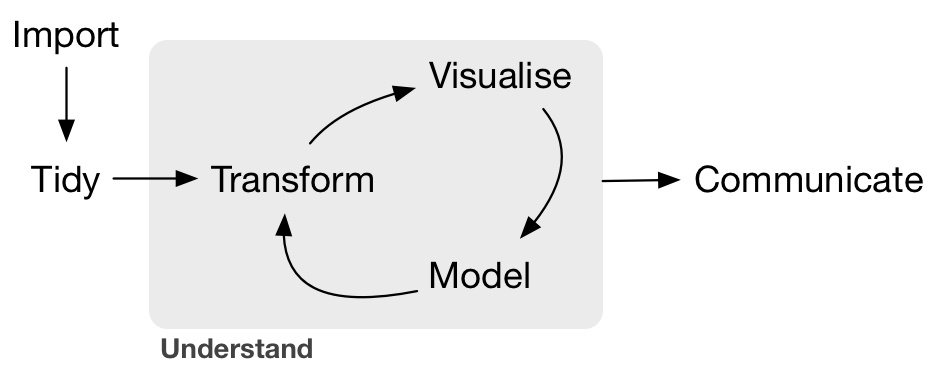
\includegraphics{img/r4ds_data-science.png}
\caption{Grolemund \& Wickham R4DS Illustration}
\end{figure}

\hypertarget{objectives-5}{%
\section{Objectives}\label{objectives-5}}

\begin{itemize}
\tightlist
\item
  Create a new repo on GitHub
\item
  Start a new R project, connected to the repo
\item
  Create a new R Markdown document
\item
  Attach necessary packages (\texttt{googlesheets4}, \texttt{tidyverse}, \texttt{here})
\item
  Use \texttt{here::here()} for simpler (and safer) file paths
\item
  Read in data from a Google sheet with the \texttt{googlesheets4} package in R
\item
  Basic data wrangling (\texttt{dplyr}, \texttt{tidyr}, etc.)
\item
  Data visualization (\texttt{ggplot2})
\item
  Publish with a useful ReadMe to share
\end{itemize}

\hypertarget{resources-8}{%
\section{Resources}\label{resources-8}}

\begin{itemize}
\tightlist
\item
  The \href{https://github.com/r-lib/here}{\texttt{here} package}
\item
  \href{https://github.com/tidyverse/googlesheets4}{googlesheets4} information
\item
  \href{https://www.tidyverse.org/blog/2017/12/workflow-vs-script/}{Project oriented workflows} by Jenny Bryan
\end{itemize}

\hypertarget{lesson-3}{%
\section{Lesson}\label{lesson-3}}

\hypertarget{set-up}{%
\subsection{Set-up:}\label{set-up}}

\begin{itemize}
\tightlist
\item
  Log in to your GitHub account and create a new repository called \texttt{sea-creature-synthesis}
\item
  Clone the repo to create a version controlled project (remember, copy \& paste the URL from the GitHub Clone / Download)
\item
  In the local project folder, create a subfolder called `data'
\item
  Copy and paste the \texttt{fish\_counts\_curated.csv} and \texttt{lobster\_counts.csv} into the `data' subfolder
\item
  Create a new R Markdown document within your \texttt{sea-creature-synthesis} project
\item
  Knit your .Rmd to html, saving as \texttt{sb\_sea\_creatures.Rmd}
\end{itemize}

\hypertarget{attach-packages-and-read-in-the-data}{%
\subsection{Attach packages and read in the data}\label{attach-packages-and-read-in-the-data}}

Attach (load) packages with \texttt{library()}:

\begin{Shaded}
\begin{Highlighting}[]
\KeywordTok{library}\NormalTok{(tidyverse)}
\KeywordTok{library}\NormalTok{(googlesheets4)}
\KeywordTok{library}\NormalTok{(here)  }
\KeywordTok{library}\NormalTok{(janitor) }
\end{Highlighting}
\end{Shaded}

Now we'll read in our files with \texttt{readr::read\_csv()}, but our files aren't in our \textbf{project root}. They're in the \texttt{data} subfolder.

Use \texttt{here::here()} to direct R where to look for files, if they're not in the project root. Not sure where that is? Type \texttt{here()} in the Console, and it will tell you!

\begin{Shaded}
\begin{Highlighting}[]
\NormalTok{here}\OperatorTok{::}\KeywordTok{here}\NormalTok{()}
\end{Highlighting}
\end{Shaded}

\texttt{"/returns/your/project/root/"}

Go ahead, find your project root!

Then use \texttt{here::here()} \emph{again} to easily locate a file somewhere outside of the exact project root. In our case, the files we want to read in are in the \texttt{data} subfolder - so we have to tell R how to get there from the root:

\begin{Shaded}
\begin{Highlighting}[]
\CommentTok{# Read in CSV files}
\NormalTok{fish_counts <-}\StringTok{ }\NormalTok{readr}\OperatorTok{::}\KeywordTok{read_csv}\NormalTok{(here}\OperatorTok{::}\KeywordTok{here}\NormalTok{(}\StringTok{"data"}\NormalTok{, }\StringTok{"fish_counts_curated.csv"}\NormalTok{))}
\NormalTok{lobster_counts <-}\StringTok{ }\NormalTok{readr}\OperatorTok{::}\KeywordTok{read_csv}\NormalTok{(here}\OperatorTok{::}\KeywordTok{here}\NormalTok{(}\StringTok{"data"}\NormalTok{, }\StringTok{"lobster_counts.csv"}\NormalTok{))}
\end{Highlighting}
\end{Shaded}

Check out the two data frames (\texttt{fish\_counts} and \texttt{lobster\_counts}).

The \texttt{fish\_counts} data frame is in pretty good shape. But the \texttt{lobster\_counts} df could use some love, because there are ``-99999'' entries indicating \texttt{NA} values, and the column names would be difficult to write code with.

When reading in the lobster data, let's:

\begin{itemize}
\tightlist
\item
  convert every ``-99999'' to an \texttt{NA}
\item
  get the column names into lower snake case using \texttt{janitor::clean\_names()}
\end{itemize}

\begin{Shaded}
\begin{Highlighting}[]
\NormalTok{lobster_counts <-}\StringTok{ }\KeywordTok{read_csv}\NormalTok{(here}\OperatorTok{::}\KeywordTok{here}\NormalTok{(}\StringTok{"curation"}\NormalTok{, }\StringTok{"lobster_counts.csv"}\NormalTok{),}
                           \DataTypeTok{na =} \StringTok{"-99999"}\NormalTok{) }\OperatorTok\StringTok{ }
\StringTok{                  }\KeywordTok{clean_names}\NormalTok{() }
\end{Highlighting}
\end{Shaded}

Look at it again to check (always look at your data) - now both data frames seem pretty coder-friendly to work with.

\hypertarget{data-wrangling}{%
\subsection{Data wrangling}\label{data-wrangling}}

\begin{itemize}
\item
  join?
\item
  filter?
\item
  unite/separate
\item
  Read in lobster data
\item
  Join with another existing data frame (or 2?)
\item
  Pivoting
\item
  Transforming / subsetting
\item
  Grouping \& summarizing (for means, sd, count)
\item
  Make a table
\item
  Make a graph
\end{itemize}

Possible new things:
complete()

\hypertarget{fun-facts-quirky-things---making-a-note-of-these-wherever-possible-for-interest-little-did-you-know-sections-3}{%
\section{Fun facts (quirky things) - making a note of these wherever possible for interest (little ``Did you know?'' sections)}\label{fun-facts-quirky-things---making-a-note-of-these-wherever-possible-for-interest-little-did-you-know-sections-3}}

\hypertarget{interludes-deep-thoughtsopenscapes-6}{%
\section{Interludes (deep thoughts/openscapes)}\label{interludes-deep-thoughtsopenscapes-6}}

\hypertarget{efficiency-tips-7}{%
\section{Efficiency Tips}\label{efficiency-tips-7}}

\bibliography{book.bib,packages.bib}


\end{document}
